\documentclass[12pt,oneside]{book}

%%%%%%%%%%%%%%%%%%%%%%%%%%%%%%%%%%%%%%%%%%%%%%%%%%%%%%%%%%%%%%%%%%%%%%%%%%%%%%%%%%%%%%%%%%%%%%%%%%%
%                                                                                                 %
% The mathematical style of these documents follows                                               %
%                                                                                                 %
% A. Thompson and B.N. Taylor. The NIST Guide for the Use of the International System of Units.   %
%    NIST Special Publication 881, 2008.                                                          %
%                                                                                                 %
% http://www.nist.gov/pml/pubs/sp811/index.cfm                                                    %
%                                                                                                 %
%%%%%%%%%%%%%%%%%%%%%%%%%%%%%%%%%%%%%%%%%%%%%%%%%%%%%%%%%%%%%%%%%%%%%%%%%%%%%%%%%%%%%%%%%%%%%%%%%%%

% $Date: 2013-11-26 10:43:59 -0500 (Tue, 26 Nov 2013) $
% $Revision: 17538 $
% $Author: gforney $

%%%%%%%%%%%%%%%%%%%%%%%%%%%%%%%%%%%%%%%%%%%%%%%%%%%%%%%%%%%%%%%%%%%%%%%%%%%%%%%%%%%%%%%%%%%%%%%%%%%
%                                                                                                 %
% The mathematical style of these documents follows                                               %
%                                                                                                 %
% A. Thompson and B.N. Taylor. The NIST Guide for the Use of the International System of Units.   %
%    NIST Special Publication 881, 2008.                                                          %
%                                                                                                 %
% http://www.nist.gov/pml/pubs/sp811/index.cfm                                                    %
%                                                                                                 %
%%%%%%%%%%%%%%%%%%%%%%%%%%%%%%%%%%%%%%%%%%%%%%%%%%%%%%%%%%%%%%%%%%%%%%%%%%%%%%%%%%%%%%%%%%%%%%%%%%%

% Packages which force the use of better TeX coding
% Mostly from http://tex.stackexchange.com/q/19264
%%\RequirePackage[l2tabu, orthodox]{nag}
%%\usepackage{fixltx2e}
%\usepackage{isomath} % Disabled for the moment because it changes the syntax for bold and roman Greek math symbols
%%\usepackage[all,warning]{onlyamsmath}
%\usepackage{strict} % Commented out for now because it is uncommon. A copy of style.sty is in Manuals/LaTeX_Style_Files/.

\usepackage{times,mathptmx}
\usepackage[pdftex]{graphicx}
\usepackage{tabularx,ragged2e,booktabs,caption}
\usepackage{multirow}
\usepackage{pdfsync}
\usepackage{tikz}
\usepackage{pgfplots}
%\pgfplotsset{compat=1.7}
\usepackage{tocloft}
\usepackage{color}
\usepackage{amsmath}
\definecolor{linknavy}{rgb}{0,0,0.50196}
\definecolor{linkred}{rgb}{1,0,0}
\definecolor{linkblue}{rgb}{0,0,1}
\usepackage{float}
\usepackage{caption}
\usepackage{graphpap}
\usepackage{rotating}
\usepackage{graphicx}
\usepackage{geometry}
\usepackage{relsize}
\usepackage{longtable}
\usepackage{lscape}
\usepackage{amssymb}
\usepackage{makeidx} % Create index at end of document
\usepackage[nottoc,notlof,notlot]{tocbibind} % Put the bibliography and index in the ToC
\usepackage{lastpage} % Automatic last page number reference.
\usepackage[T1]{fontenc}
\usepackage{enumerate}
\usepackage{upquote}
\usepackage{moreverb}
\usepackage{xfrac}
\usepackage{cite}

\newcommand{\nopart}{\expandafter\def\csname Parent-1\endcsname{}} % To fix table of contents in pdf.
\newcommand{\ct}{\tt\small} % eventually will be deprecated due to http://www.tex.ac.uk/cgi-bin/texfaq2html?label=2letterfontcmd
\newcommand{\textct}[1]{\texttt{\small #1}}

\usepackage{tocstyle} % Fix table of contents sections from overlapping section titles
\usetocstyle{standard}
\usepackage{siunitx}
\sisetup{
    detect-all = true,
    input-decimal-markers = {.},
    input-ignore = {,},
    inter-unit-product = \ensuremath{{}\cdot{}},
    multi-part-units = repeat,
    number-unit-product = \text{~},
    per-mode = fraction,
    separate-uncertainty = true,
}

\usepackage{listings}
\usepackage{textcomp}
\definecolor{lbcolor}{rgb}{0.96,0.96,0.96}
\lstset{
    %backgroundcolor=\color{lbcolor},
    tabsize=4,
    rulecolor=,
    language=Fortran,
        basicstyle=\footnotesize\ttfamily,
        upquote=true,
        aboveskip={\baselineskip},
        belowskip={\baselineskip},
        columns=fixed,
        extendedchars=true,
        breaklines=true,
        breakatwhitespace=true,
        frame=none,
        showtabs=false,
        showspaces=false,
        showstringspaces=false,
        identifierstyle=\ttfamily,
        keywordstyle=\color[rgb]{0,0,0},
        commentstyle=\color[rgb]{0,0,0},
        stringstyle=\color[rgb]{0,0,0},
}

\usepackage[pdftex,
        colorlinks=true,
        urlcolor=linkblue,     % \href{...}{...} external (URL)
        citecolor=linkred,     % citation number colors
        linkcolor=linknavy,    % \ref{...} and \pageref{...}
        pdfproducer={pdflatex},
        pdfpagemode=UseNone,
        bookmarksopen=true,
        plainpages=false,
        verbose]{hyperref}

% The Following commented code makes the ``Draft'' watermark on each page.
%\usepackage{eso-pic}
%\usepackage{type1cm}
%\makeatletter
%   \AddToShipoutPicture{
%     \setlength{\@tempdimb}{.5\paperwidth}
%     \setlength{\@tempdimc}{.5\paperheight}
%     \setlength{\unitlength}{1pt}
%     \put(\strip@pt\@tempdimb,\strip@pt\@tempdimc){
%     \makebox(0,0){\rotatebox{45}{\textcolor[gray]{0.75}{\fontsize{8cm}\selectfont{RC6}}}}}
% }
%\makeatother

\setlength{\textwidth}{6.5in}
\setlength{\textheight}{9.0in}
\setlength{\topmargin}{0.in}
\setlength{\headheight}{0.pt}
\setlength{\headsep}{0.in}
\setlength{\parindent}{0.25in}
\setlength{\oddsidemargin}{0.0in}
\setlength{\evensidemargin}{0.0in}
\setlength{\leftmargini}{\parindent} % Controls the indenting of the "bullets" in a list
\setlength{\cftsecnumwidth}{0.45in}
\setlength{\cftsubsecnumwidth}{0.5in}
\setlength{\cftfignumwidth}{0.45in}
\setlength{\cfttabnumwidth}{0.45in}

\newcommand{\titlesigs}
{
\small
\flushright{U.S. Department of Commerce \\
{\em Penny Pritzker, Secretary} \\
\hspace{1in} \\
National Institute of Standards and Technology \\
{\em Willie May, Under Secretary of Commerce for Standards and Technology and Acting Director} }
}

% commands to use for "official" cover and title pages
% see smokeview verification guide to see how they are used

\newcommand{\headerA}[1]{
\flushright{
\fontsize{20}{24}\selectfont
\bf{NIST Special Publication #1}}
}

\newcommand{\headerB}[1]{
\flushright{
\fontsize{28}{33.6}\selectfont
\bf{#1}
}
}

\newcommand{\headerC}[1]{
\vspace{.5in}
\flushright{\fontsize{14}{16.8}\selectfont
#1}
}

\frenchspacing

\newcommand{\dod}[2]{\frac{\partial #1}{\partial #2}}
\newcommand{\DoD}[2]{\frac{\mathrm{D} #1}{\mathrm{D} #2}}
\newcommand{\dsods}[2]{\frac{\partial^2 #1}{\partial #2^2}}
\renewcommand{\d}{\,\mathrm{d}}
\newcommand{\dx}{\delta x}
\newcommand{\dy}{\delta y}
\newcommand{\dz}{\delta z}
\newcommand{\degF}{$^\circ$F}
\newcommand{\degC}{$^\circ$C}
\newcommand{\x}{x}
\newcommand{\y}{y}
\newcommand{\z}{z}
\newcommand{\dt}{\delta t}
\newcommand{\dn}{\delta n}
\newcommand{\cH}{H}
\newcommand{\hu}{u}
\newcommand{\hv}{v}
\newcommand{\hw}{w}
\newcommand{\la}{\lambda}
\newcommand{\bO}{{\Omega}}
\newcommand{\bo}{{\mathbf{\omega}}}
\newcommand{\btau}{\mathbf{\tau}}
\newcommand{\bdelta}{{\mathbf{\delta}}}
\newcommand{\sumyw}{\sum (Y_\alpha/W_\alpha)}
\newcommand{\oW}{\overline{W}}
\newcommand{\om}{\ensuremath{\omega}}
\newcommand{\omx}{\omega_x}
\newcommand{\omy}{\omega_y}
\newcommand{\omz}{\omega_z}
\newcommand{\erf}{\hbox{erf}}
\newcommand{\erfc}{\hbox{erfc}}
\newcommand{\bF}{{\mathbf{F}}}
\newcommand{\bG}{{\mathbf{G}}}
\newcommand{\bof}{{\mathbf{f}}}
\newcommand{\bq}{{\mathbf{q}}}
\newcommand{\br}{{\mathbf{r}}}
\newcommand{\bu}{{\mathbf{u}}}
\newcommand{\bx}{{\mathbf{x}}}
\newcommand{\bk}{{\mathbf{k}}}
\newcommand{\bv}{{\mathbf{v}}}
\newcommand{\bg}{{\mathbf{g}}}
\newcommand{\bn}{{\mathbf{n}}}
\newcommand{\bS}{{\mathbf{S}}}
\newcommand{\bW}{\overline{W}}
\newcommand{\dS}{d{\mathbf{S}}}
\newcommand{\bs}{{\mathbf{s}}}
\newcommand{\bI}{{\mathbf{I}}}
\newcommand{\hp}{H}
\newcommand{\trho}{\tilde{\rho}}
\newcommand{\dph}{{\delta\phi}}
\newcommand{\dth}{{\delta\theta}}
\newcommand{\tp}{\tilde{p}}
\newcommand{\bp}{\overline{p}}
\newcommand{\dQ}{\dot{Q}}
\newcommand{\dq}{\dot{q}}
\newcommand{\dbq}{\dot{\mathbf{q}}}
\newcommand{\dm}{\dot{m}}
\newcommand{\ha}{\frac{1}{2}}
\newcommand{\ft}{\frac{4}{3}}
\newcommand{\ot}{\frac{1}{3}}
\newcommand{\fofi}{\frac{4}{5}}
\newcommand{\of}{\frac{1}{4}}
\newcommand{\twth}{\frac{2}{3}}
\newcommand{\R}{R}
\newcommand{\be}{\begin{equation}}
\newcommand{\ee}{\end{equation}}
\newcommand{\RE}{\hbox{Re}}
\newcommand{\LE}{\hbox{Le}}
\newcommand{\PR}{\hbox{Pr}}
\newcommand{\PE}{\hbox{Pe}}
\newcommand{\NU}{\hbox{Nu}}
\newcommand{\SC}{\hbox{Sc}}
\newcommand{\SH}{\hbox{Sh}}
\newcommand{\WE}{\hbox{We}}
\newcommand{\COTWO}{\text{\tiny \hbox{CO}$_2$}}
\newcommand{\HTWOO}{\text{\tiny \hbox{H}$_2$\hbox{O}}}
\newcommand{\OTWO}{\text{\tiny \hbox{O}$_2$}}
\newcommand{\NTWO}{\text{\tiny \hbox{N}$_2$}}
\newcommand{\CO}{\text{\tiny \hbox{CO}}}
\newcommand{\F}{\text{\tiny \hbox{F}}}
\newcommand{\C}{\text{\tiny \hbox{C}}}
\newcommand{\Hy}{\text{\tiny \hbox{H}}}
\newcommand{\So}{\text{\tiny \hbox{S}}}
\newcommand{\M}{\text{\tiny \hbox{M}}}
\newcommand{\xx}{\text{\tiny \hbox{x}}}
\newcommand{\yy}{\text{\tiny \hbox{y}}}
\newcommand{\zz}{\text{\tiny \hbox{z}}}
\newcommand{\smvlines}{115~000}

\newcommand{\calH}{\mathcal{H}}
\newcommand{\calR}{\mathcal{R}}

\newcommand{\dif}{\mathrm{d}}
\newcommand{\Div}{\nabla\cdot}
\newcommand{\D}{\mbox{D}}
\newcommand{\mhalf}{\mbox{$\frac{1}{2}$}}
\newcommand{\thalf}{\mbox{\tiny $\frac{1}{2}$}}
\newcommand{\tripleprime}{{\prime\prime\prime}}
\newcommand{\ppp}{{\prime\prime\prime}}
\newcommand{\pp}{{\prime\prime}}

\newcommand{\superscript}[1]{\ensuremath{^{\textrm{\tiny #1}}}}
\newcommand{\subscript}[1]{\ensuremath{_{\textrm{\tiny #1}}}}

\newcommand{\rb}[1]{\raisebox{1.5ex}[0pt]{#1}}

\newcommand{\Ra}{$\Rightarrow$}
\newcommand{\hhref}[1]{\href{#1}{{\tt #1}}}
\newcommand{\fdsinput}[1]{{\scriptsize\verbatiminput{../../Verification/Visualization/#1}}}

\definecolor{AQUAMARINE}{rgb}{0.49804,1.00000,0.83137}
\definecolor{ANTIQUE WHITE}{rgb}{0.98039,0.92157,0.84314}
\definecolor{BEIGE}{rgb}{0.96078,0.96078,0.86275}
\definecolor{BLACK}{rgb}{0.00000,0.00000,0.00000}
\definecolor{BLUE}{rgb}{0.00000,0.00000,1.00000}
\definecolor{BLUE VIOLET}{rgb}{0.54118,0.16863,0.88627}
\definecolor{BRICK}{rgb}{0.61176,0.40000,0.12157}
\definecolor{BROWN}{rgb}{0.64706,0.16471,0.16471}
\definecolor{BURNT SIENNA}{rgb}{0.54118,0.21176,0.05882}
\definecolor{BURNT UMBER}{rgb}{0.54118,0.20000,0.14118}
\definecolor{CADET BLUE}{rgb}{0.37255,0.61961,0.62745}
\definecolor{CHOCOLATE}{rgb}{0.82353,0.41176,0.11765}
\definecolor{COBALT}{rgb}{0.23922,0.34902,0.67059}
\definecolor{CORAL}{rgb}{1.00000,0.49804,0.31373}
\definecolor{CYAN}{rgb}{0.00000,1.00000,1.00000}
\definecolor{DIMGRAY }{rgb}{0.41176,0.41176,0.41176}
\definecolor{EMERALD GREEN}{rgb}{0.00000,0.78824,0.34118}
\definecolor{FIREBRICK}{rgb}{0.69804,0.13333,0.13333}
\definecolor{FLESH}{rgb}{1.00000,0.49020,0.25098}
\definecolor{FOREST GREEN}{rgb}{0.13333,0.54510,0.13333}
\definecolor{GOLD }{rgb}{1.00000,0.84314,0.00000}
\definecolor{GOLDENROD}{rgb}{0.85490,0.64706,0.12549}
\definecolor{GRAY}{rgb}{0.50196,0.50196,0.50196}
\definecolor{GREEN}{rgb}{0.00000,1.00000,0.00000}
\definecolor{GREEN YELLOW}{rgb}{0.67843,1.00000,0.18431}
\definecolor{HONEYDEW}{rgb}{0.94118,1.00000,0.94118}
\definecolor{HOT PINK}{rgb}{1.00000,0.41176,0.70588}
\definecolor{INDIAN RED}{rgb}{0.80392,0.36078,0.36078}
\definecolor{INDIGO}{rgb}{0.29412,0.00000,0.50980}
\definecolor{IVORY}{rgb}{1.00000,1.00000,0.94118}
\definecolor{IVORY BLACK}{rgb}{0.16078,0.14118,0.12941}
\definecolor{KELLY GREEN}{rgb}{0.00000,0.50196,0.00000}
\definecolor{KHAKI}{rgb}{0.94118,0.90196,0.54902}
\definecolor{LAVENDER}{rgb}{0.90196,0.90196,0.98039}
\definecolor{LIME GREEN}{rgb}{0.19608,0.80392,0.19608}
\definecolor{MAGENTA}{rgb}{1.00000,0.00000,1.00000}
\definecolor{MAROON}{rgb}{0.50196,0.00000,0.00000}
\definecolor{MELON}{rgb}{0.89020,0.65882,0.41176}
\definecolor{MIDNIGHT BLUE}{rgb}{0.09804,0.09804,0.43922}
\definecolor{MINT}{rgb}{0.74118,0.98824,0.78824}
\definecolor{NAVY}{rgb}{0.00000,0.00000,0.50196}
\definecolor{OLIVE}{rgb}{0.50196,0.50196,0.00000}
\definecolor{OLIVE DRAB}{rgb}{0.41961,0.55686,0.13725}
\definecolor{ORANGE}{rgb}{1.00000,0.50196,0.00000}
\definecolor{ORANGE RED}{rgb}{1.00000,0.27059,0.00000}
\definecolor{ORCHID}{rgb}{0.85490,0.43922,0.83922}
\definecolor{PINK}{rgb}{1.00000,0.75294,0.79608}
\definecolor{POWDER BLUE}{rgb}{0.69020,0.87843,0.90196}
\definecolor{PURPLE}{rgb}{0.50196,0.00000,0.50196}
\definecolor{RASPBERRY}{rgb}{0.52941,0.14902,0.34118}
\definecolor{RED}{rgb}{1.00000,0.00000,0.00000}
\definecolor{ROYAL BLUE}{rgb}{0.25490,0.41176,0.88235}
\definecolor{SALMON}{rgb}{0.98039,0.50196,0.44706}
\definecolor{SANDY BROWN}{rgb}{0.95686,0.64314,0.37647}
\definecolor{SEA GREEN}{rgb}{0.32941,1.00000,0.62353}
\definecolor{SEPIA}{rgb}{0.36863,0.14902,0.07059}
\definecolor{SIENNA}{rgb}{0.62745,0.32157,0.17647}
\definecolor{SILVER}{rgb}{0.75294,0.75294,0.75294}
\definecolor{SKY BLUE}{rgb}{0.52941,0.80784,0.92157}
\definecolor{SLATEBLUE}{rgb}{0.41569,0.35294,0.80392}
\definecolor{SLATE GRAY}{rgb}{0.43922,0.50196,0.56471}
\definecolor{SPRING GREEN}{rgb}{0.00000,1.00000,0.49804}
\definecolor{STEEL BLUE}{rgb}{0.27451,0.50980,0.70588}
\definecolor{TAN}{rgb}{0.82353,0.70588,0.54902}
\definecolor{TEAL}{rgb}{0.00000,0.50196,0.50196}
\definecolor{THISTLE}{rgb}{0.84706,0.74902,0.84706}
\definecolor{TOMATO }{rgb}{1.00000,0.38824,0.27843}
\definecolor{TURQUOISE}{rgb}{0.25098,0.87843,0.81569}
\definecolor{VIOLET}{rgb}{0.93333,0.50980,0.93333}
\definecolor{VIOLET RED}{rgb}{0.81569,0.12549,0.56471}
\definecolor{WHITE}{rgb}{1.00000,1.00000,1.00000}
\definecolor{YELLOW}{rgb}{1.00000,1.00000,0.00000}

\pgfplotsset{
	colormap={blackwhite}{[5pt]
		rgb255(0pt)=(0,0,255); 
		rgb255(100pt)=(0,255,255); 
		rgb255(200pt)=(0,255,0); 
		rgb255(300pt)=(255,255,0); 
		rgb255(400pt)=(255,0,0)
	},
} % defines smokeview colorbar


\floatstyle{boxed}
\newfloat{notebox}{H}{lon}
\newfloat{warning}{H}{low}

% Set default longtable alignment
\setlength\LTleft{0pt}
\setlength\LTright{0pt}


% Load packages
\usepackage{graphicx}
\usepackage[super]{nth}
\usepackage{placeins}
\usepackage{units}
\usepackage[percent]{overpic}

% Rename chapter headings
\renewcommand{\chaptername}{Section}
\renewcommand{\bibname}{References}

% Math shortcuts
\renewcommand{\sb}[1]{_\mathrm{#1}}
\renewcommand{\C}{\mbox{C}}
\renewcommand{\H}{\mbox{H}}
\renewcommand{\O}{\mbox{O}}
\newcommand{\N}{\mbox{N}}

% Center all figures
\makeatletter
\g@addto@macro\@floatboxreset\centering
\makeatother

\begin{document}

\bibliographystyle{unsrt}
\pagestyle{empty}

\begin{minipage}[t][9in][s]{6.25in}

\headerB{
Impact of Hose Streams on Air Flows inside a Structure
}

\headerC{
\flushright{
Daniel Madrzykowski \\
Craig G. Weinschenk \\
Kristopher J. Overholt \\
{\em Fire Research Division \\
Engineering Laboratory \\
Gaithersburg, Maryland, USA} \\ }
}

\flushright{\today \\
}

\vfill

\flushright{

\includegraphics[width=2.in]{../../../../../Bibliography/nistident_flright_vec} \\[.3in]
}

\titlesigs

\end{minipage}

\newpage

\frontmatter

\pagestyle{plain}
\pagenumbering{roman}

\cleardoublepage
\phantomsection
\addcontentsline{toc}{chapter}{Contents}
\tableofcontents

\cleardoublepage
\phantomsection
\addcontentsline{toc}{chapter}{List of Figures}
\listoffigures

\cleardoublepage
\phantomsection
\addcontentsline{toc}{chapter}{List of Tables}
\listoftables

\chapter{List of Acronyms}

\begin{tabbing}
\hspace{1.5in} \= \\
FDS \> Fire Dynamics Simulator \\
HGL \> Hot Gas Layer \\
HRR \> Heat Release Rate \\
HRRPUA \> Heat Release Rate per Unit Area \\
NIST \> National Institute of Standards and Technology \\
\end{tabbing}

\mainmatter

\chapter{Introduction}
\label{chap:Introduction}
NIST has conducted a significant amount of research examining how ventilation affects the growth and spread of fire within structures and how the air flow to the fire may be controlled to limit or delay the growth of the fire. The studies have resulted in guidance to the fire service regarding ventilation tactics. However, ventilation tactics alone will not result in the complete extinguishment of the fire; fire suppression with hose streams is also needed.

Fire suppression tactics using hose streams also affect the ventilation in a structure and can impact the movement of smoke and heat through a structure as vents are made to advance the line or if ventilation inducing hand line tactics are in practice. This research addressing the coordination of suppression tactics and the impact on ventilation is needed to complete recommendations on fire control tactics to appropriate standards, education, and training documents.

This report is concerned with examining the impact of hose stream selection and the pattern in which the stream is applied on the ventilation inside a structure with various flow path configurations. Two types of experiments were conducted in order to examine the impact. First, cold flow tests were performed. These tests involved using a 0.46 m (18 in) diameter positive pressure ventilation (PPV) fan to move air through a structure with various flow path configurations. The second type of experiment involved flowing water using various stream and application patterns into a structure with flow path configurations similar to the cold flow test configurations. Air velocities measured during the hose flow experiments were compared to the velocities measured during the cold flow tests to determine the impact of hose stream and application pattern combinations on ventilation throughout the structure relative to the impact of using a 0.46 m (18 in) diameter PPV fan to move air throughout the structure. 

Three types of hose streams were each applied in four different fashions during each set of hose flow experiments. The three types of hose stream patterns studied, pictured in Figure~\ref{fig:hose_streams}, were straight stream, narrow fog stream, and wide fog stream. Water was flowed into the structure by having the hose in a static, fixed position, moving the hose line left-to-right across the room in a sweeping motion, and rotating the hose line in both the clockwise and counterclockwise directions.

\begin{figure}[!ht]
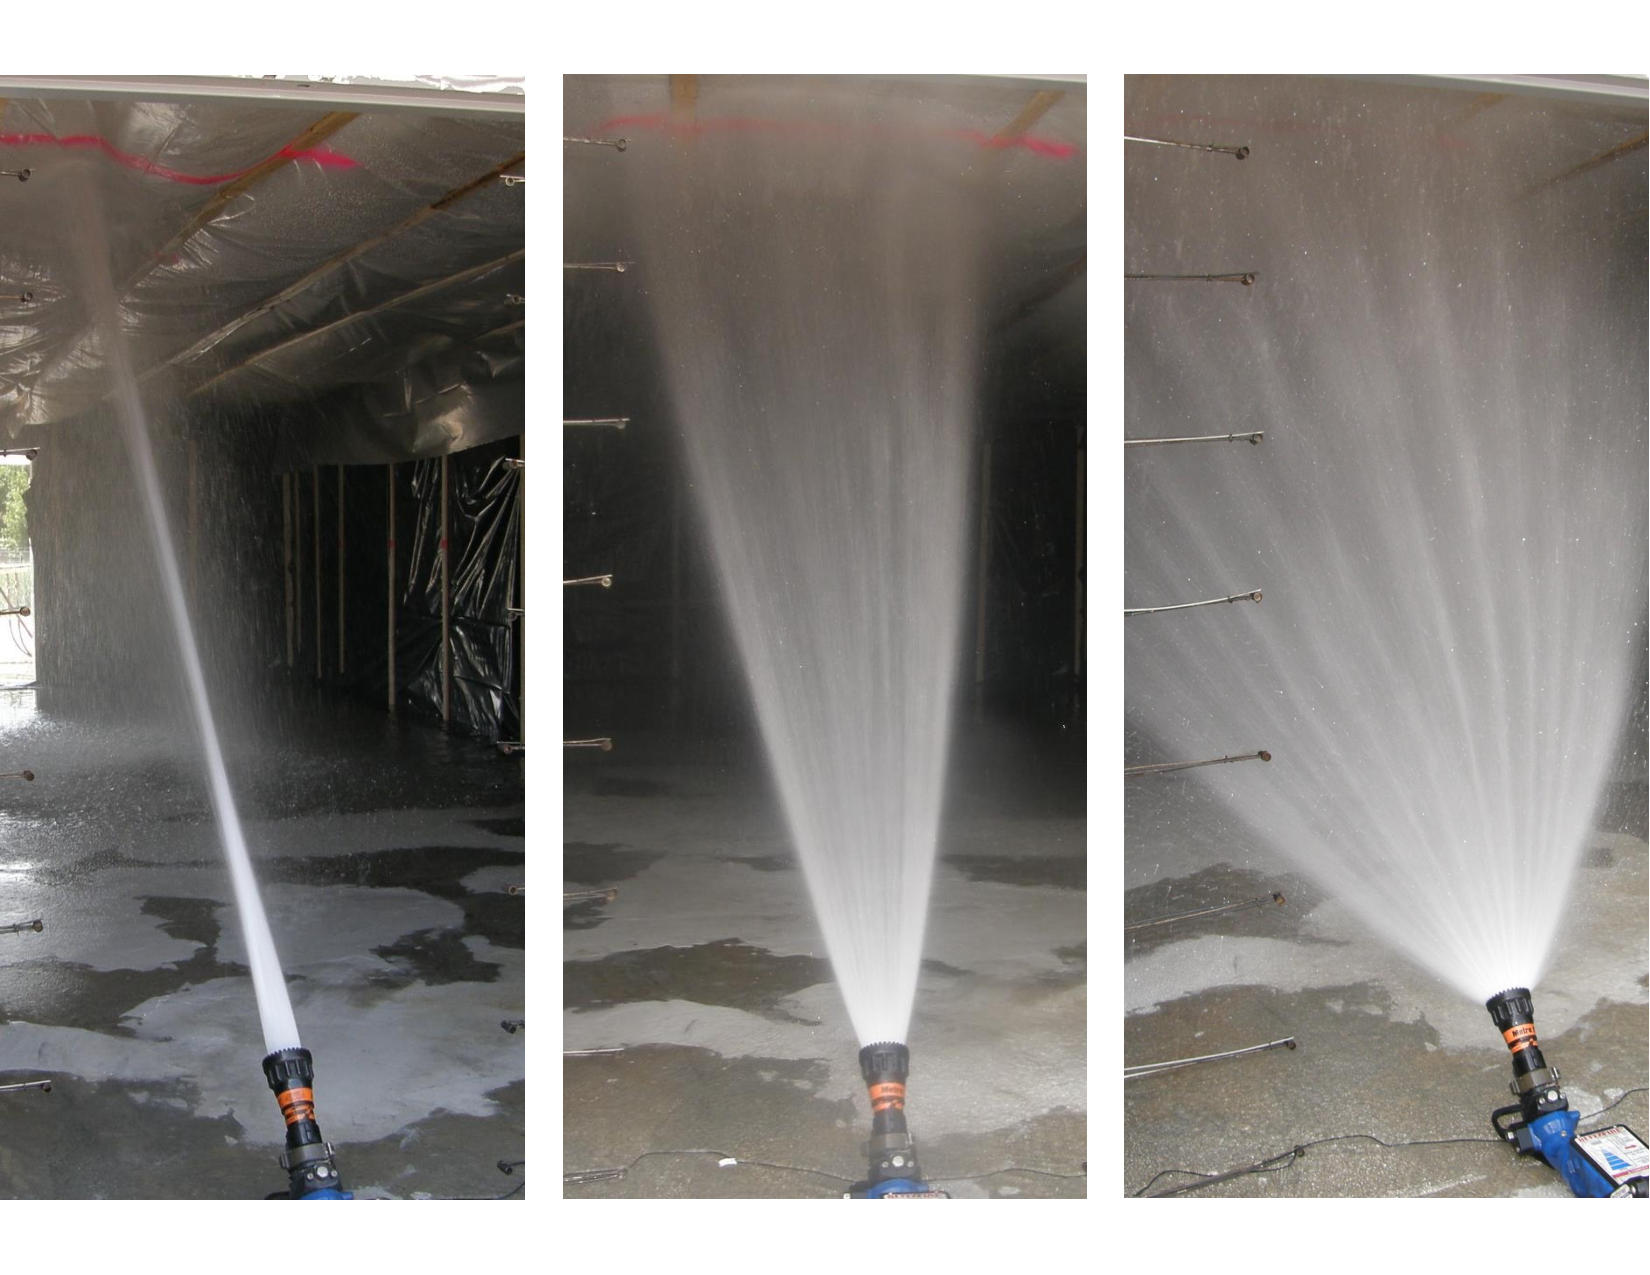
\includegraphics[width=6in]{../Pictures/hose_streams.pdf}
\caption[Different Hose Stream Patterns]{The three types of hose stream patterns used during the water flow experiments from left to right: straight stream, narrow fog stream, and wide fog stream.}
\label{fig:hose_streams}
\end{figure}
\FloatBarrier

\section{Background}
\label{sec:Background}
%http://www.tft.com/literature/library/files/bfa.pdf
Bill Nelson and Keith Royer strongly recommend that the rotation be clockwise as viewed from the nozzle operator’s position. From many experiments it was determined that a clockwise rotation is more effective than a counterclockwise rotation. They say that:
1. Clockwise rotation is safer since it drive smoke, gases, and flames away from the nozzle.
Counterclockwise rotation does just the opposite.
2. Clockwise rotation produces steam with an active rolling action. Counterclockwise rotation
produces steam with an inactive and lazy action.
3. A clockwise rotation produces a faster knockdown time.

\chapter{Experimental Setup}
\label{chap:Experimental_Setup}

\section{Experimental Structure}
\label{sec:Experimental_Structure}
This series of field experiments was conducted in two structures located at the Delaware County Emergency Services Training Center in Sharon Hill, PA. 

\subsection{Construction}
\label{sec:Construction}
Two concrete structures were built on a concrete slab as shown in Fig.~\ref{fig:struct_pics}. They were designed to simulate a single-story and a two-story residential structure.  The first floor of each structure had an outer wall composed of interlocking concrete blocks of dimensions 0.61 m x 0.61 m 0.61 m (2 ft x 2ft x 2ft). The interior dimensions of each structure were 6.1 m (20 ft) wide, 11 m (36 ft) long and 2.4 m (8 ft) high.  The joints and gaps between the blocks were filled with high temperature insulation.

The interior walls of the first floor of each structure were framed with steel studs and track.  The studs were set to 0.40 m (16 in) centers.  The ceiling/floor support was composed of wood truss joist I-beams (TJIs) with a 299 mm (11.75 in) depth.  The TJI was composed of laminated veneer lumber flanges with a cross section of 29 mm (1.125 in) x 44 mm (1.75 in) and an 11 mm (0.43 in) thick oriented strand board web as shown in Figure  XX .  Tongue and grove, 18.3 mm (0.72 in) thick, oriented strand board was screwed (nailed?) to the top of the TJIs.

The second story of the two level structure was built on the wood floor assembly as described above. The walls were framed with wood studs etc...

The interior walls of the burn room were lined with 13 mm (0.5 in) thick cement board.  The ceiling of the burn room was the exposed ``floor assembly".  The walls of the hallway and entry foyer were composed of 16 mm (0.625 in) Type X gypsum room. The ceiling of the hallway and entry foyer was composed of two layers of 13 mm (0.5 in) thick cement board.  

\begin{figure}[!ht]
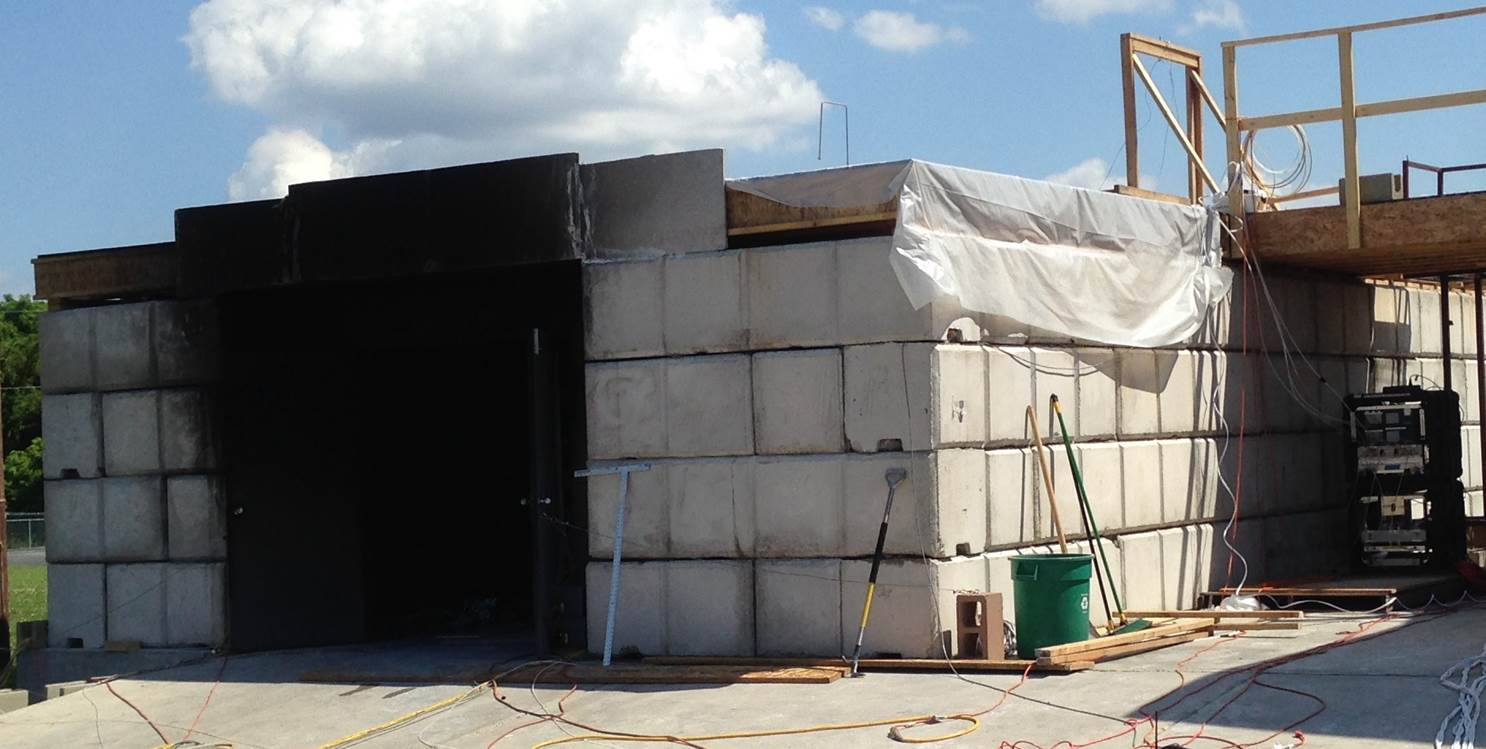
\includegraphics[width=6in]{../Pictures/east_structure}
\\~\\
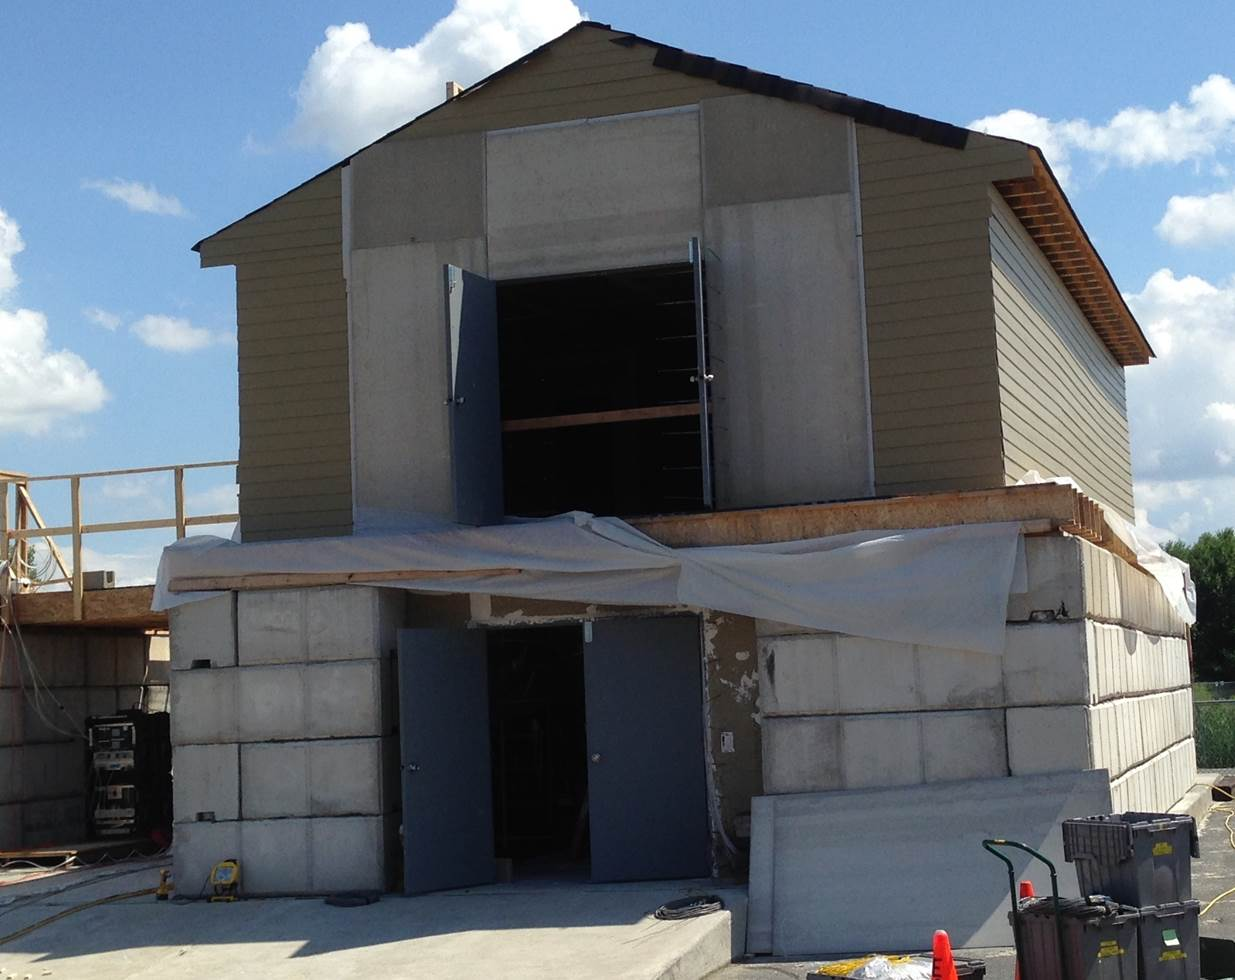
\includegraphics[width=6in]{../Pictures/west_structure}
\caption[East and West Test Structures]{East (top) and West (bottom) Test Structures}
\label{fig:struct_pics}
\end{figure}

\begin{figure}[!ht]
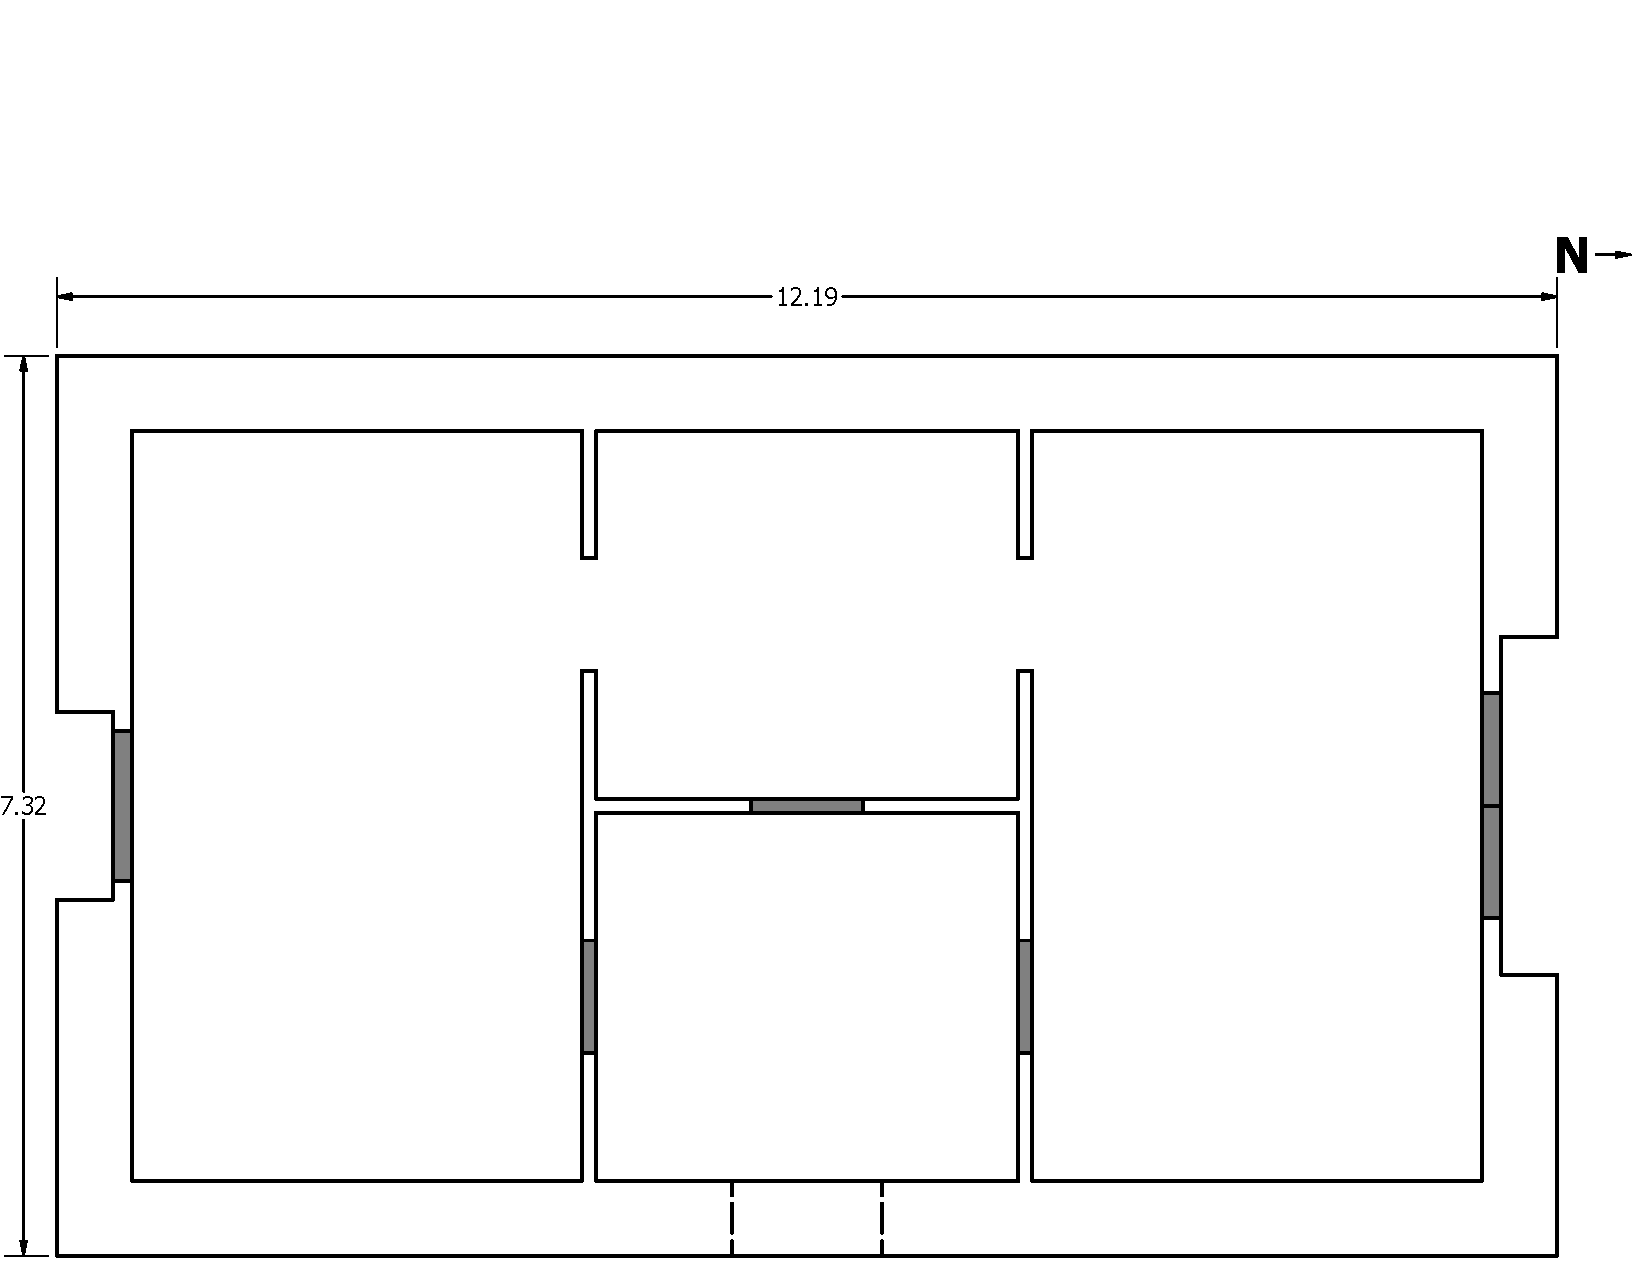
\includegraphics[trim=0cm 0cm 0.25cm 4cm, clip=true, width=6in]{../Drawings/East_Structure_Metric_Simple}
\caption[East Structure Layout]{East Structure floor layout. All dimensions are in meters.}
\label{fig:east_general_plan}
\end{figure}

\clearpage

\begin{figure}[!ht]
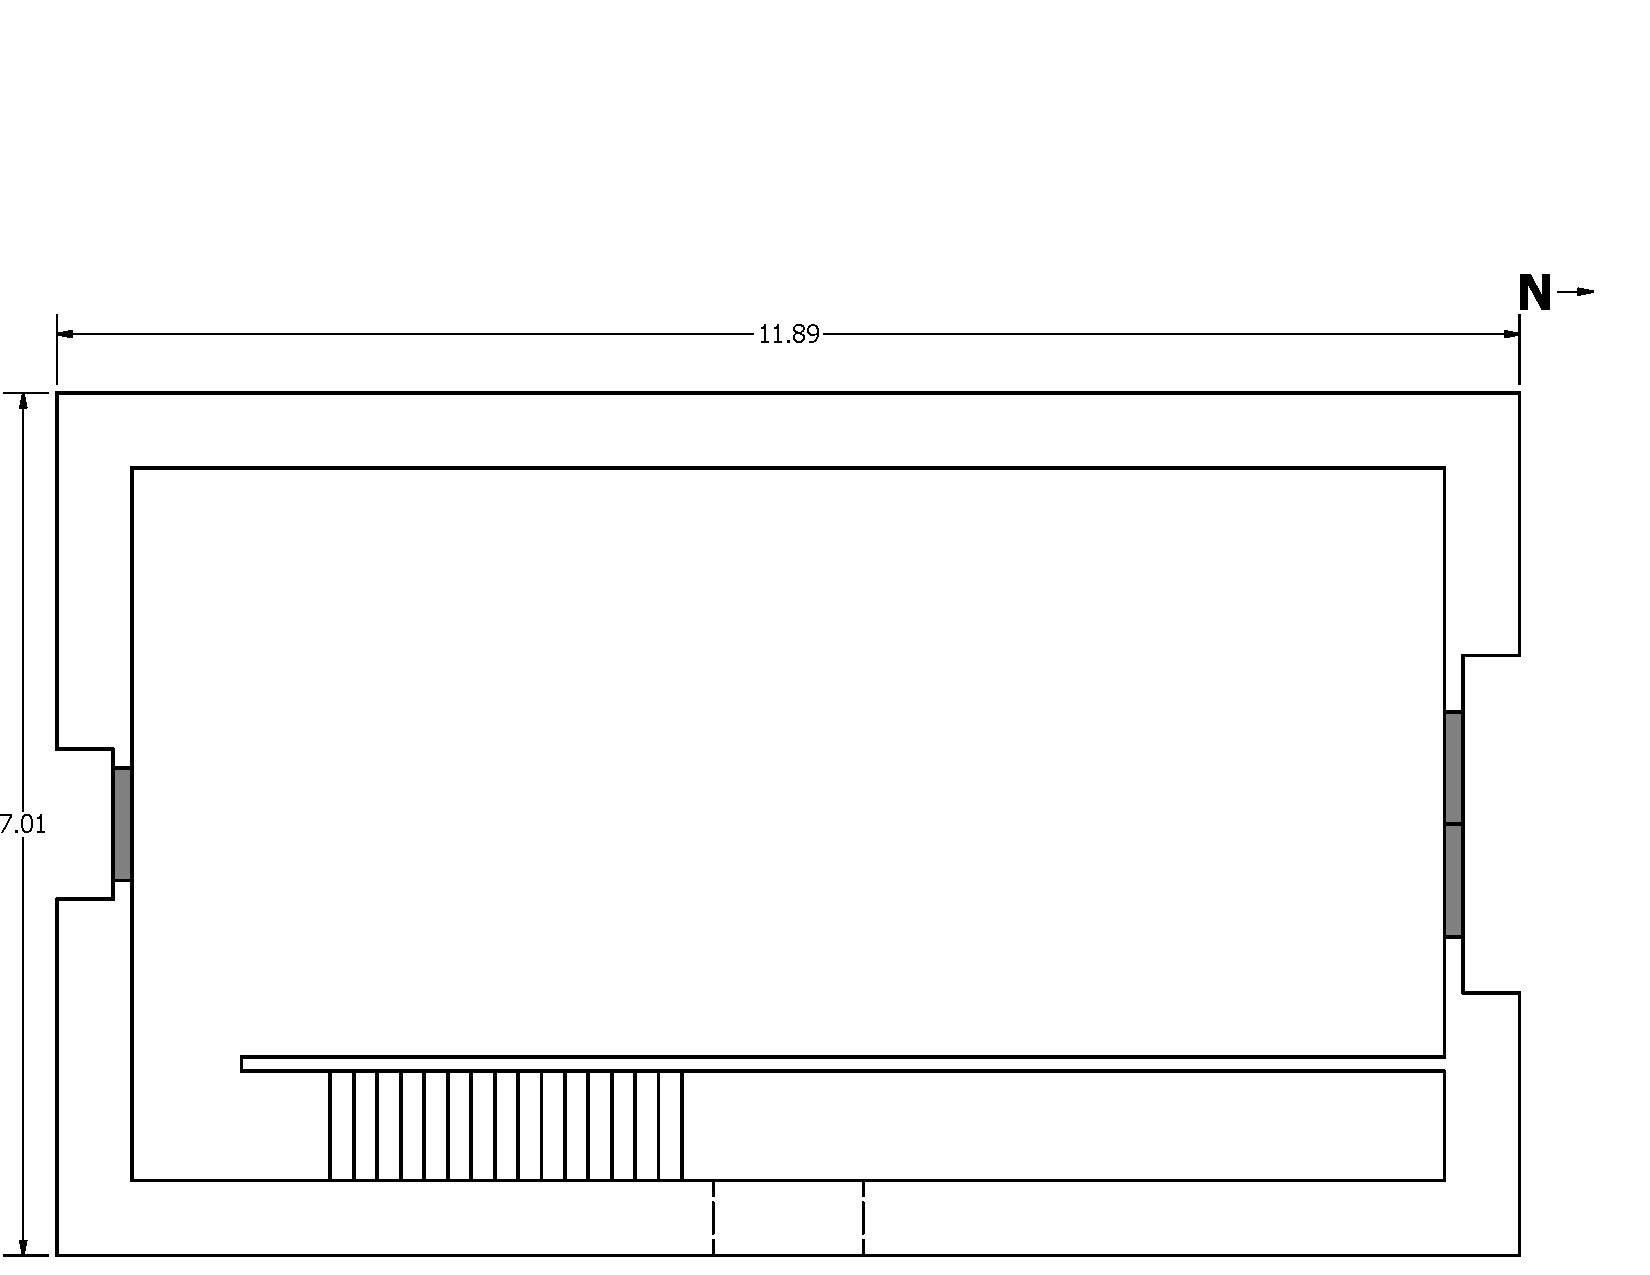
\includegraphics[trim=0cm 0cm 0.75cm 4.5cm, clip=true, width=6in]{../Drawings/West_Structure_1st_Floor_Metric_Simple}
\\
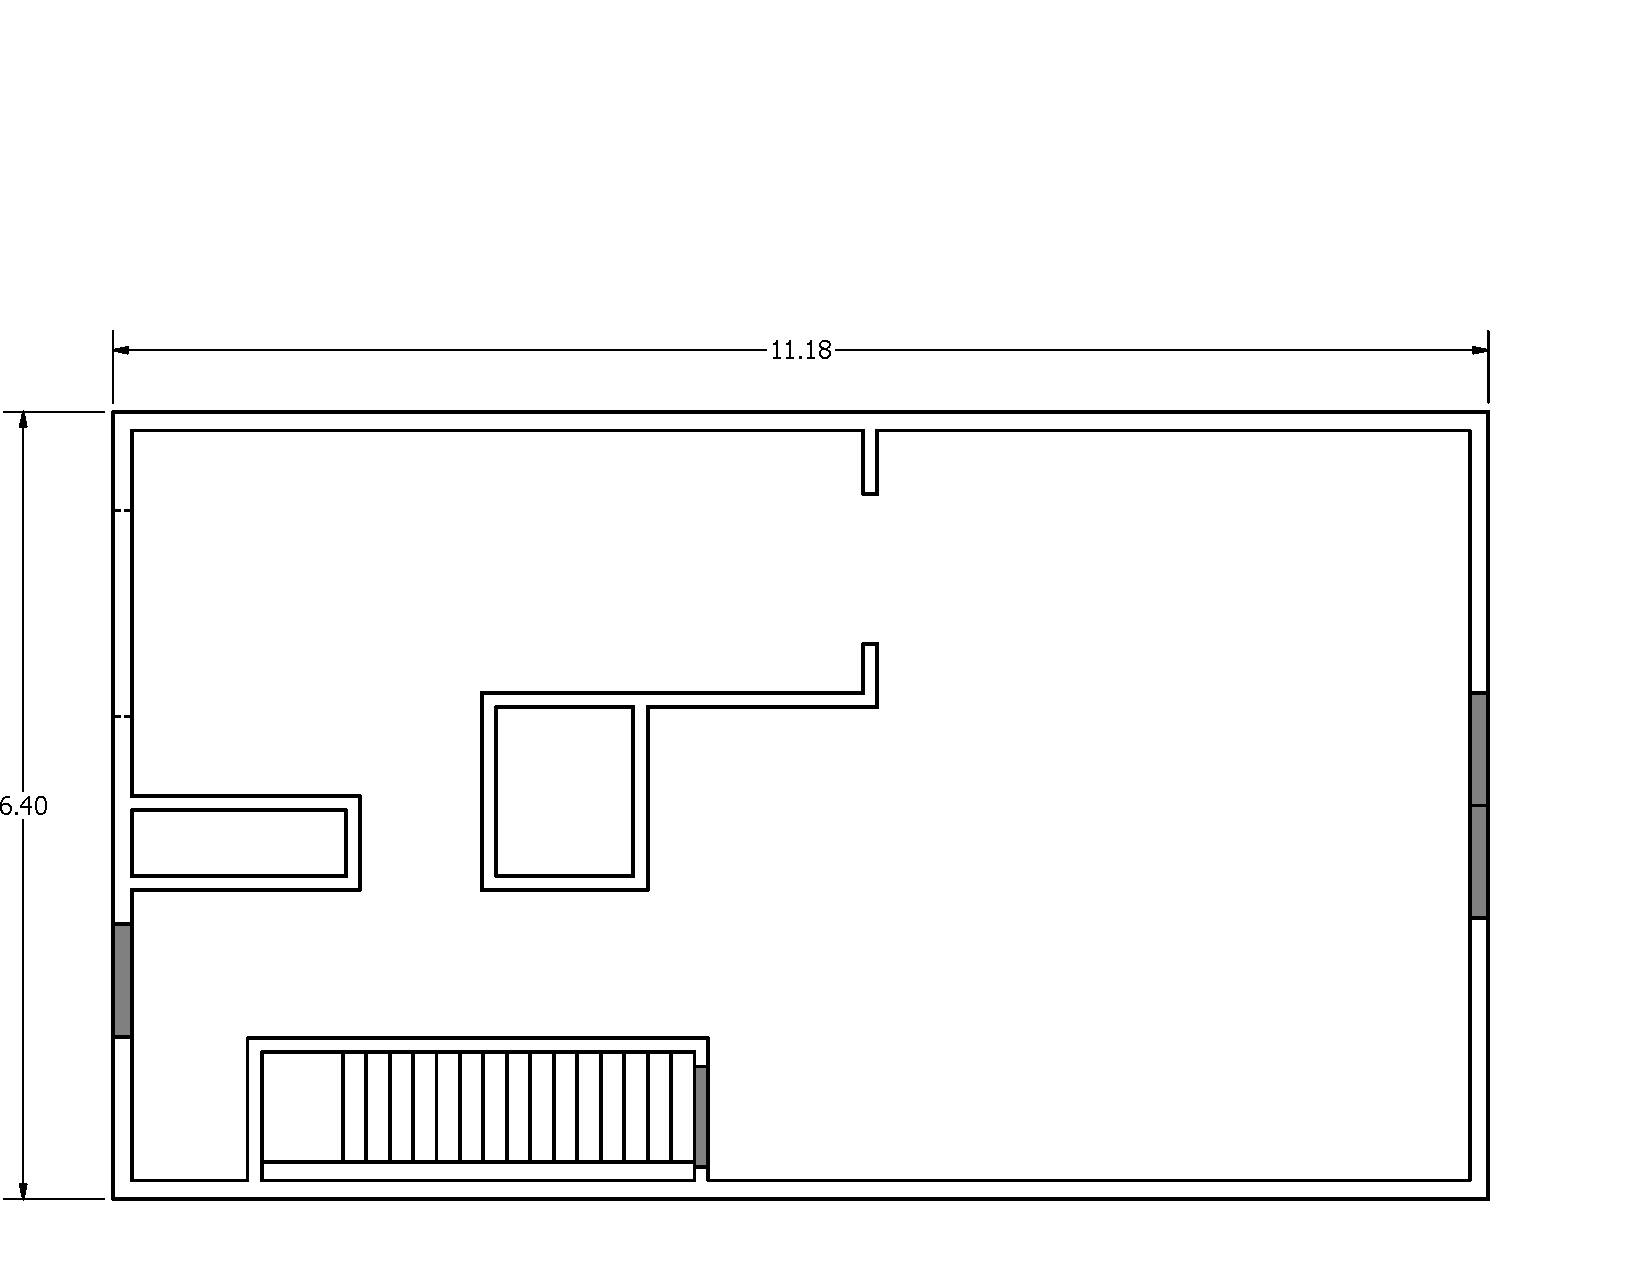
\includegraphics[trim=0cm 0cm 0.75cm 5.0cm, clip=true, width=6in]{../Drawings/West_Structure_2nd_Floor_Metric_Simple}
\caption[West Structure First and Second Floor Layout]{West Structure first floor (top) and second floor (bottom) layouts. All dimensions are in meters.}
\label{fig:west_general_plan}
\end{figure}

\clearpage

\subsection{Instrumentation}
\label{sec:Instrumentation}
Schematic plan overviews of the instrumentation in the East and West Structures are provided in Fig.~\ref{fig:east_instrumentation} and Fig.~\ref{fig:west_instrumentation}. There is a discussion of uncertainties for each measurement below in Section~\ref{sec:Uncertainty}. Gas velocity was measured at various doorways using differential pressure transducers connected to bi-directional velocity probes~\cite{McCaffrey:Combustion_and_Flame}. Each set of BDPs contained 8 probes located at distances of 0.08 m, 0.34 m, 0.61 m, 0.88 m, 1.15 m, 1.42 m, 1.68 m, and 1.95 m below the soffit of the corresponding doorway. Fig.~\ref{fig:BDPs} shows a picture of two sets of BDPs, A5 and A6, located at each double door on the first floor of the West Structure. A single thermocouple was attached to each bi-directional probe. The thermocouples that are used with the bi-directional probes are exposed-bead, Chromel-Alumel (type K) with a 1.0 mm (0.04 in) diameter. Starting with the exposed bead, the thermocouple wire was sheathed in a 3.2 mm (0.13 in) diameter Inconel shield, 0.76 m (2.5 ft) in length.

\begin{figure}[!ht]
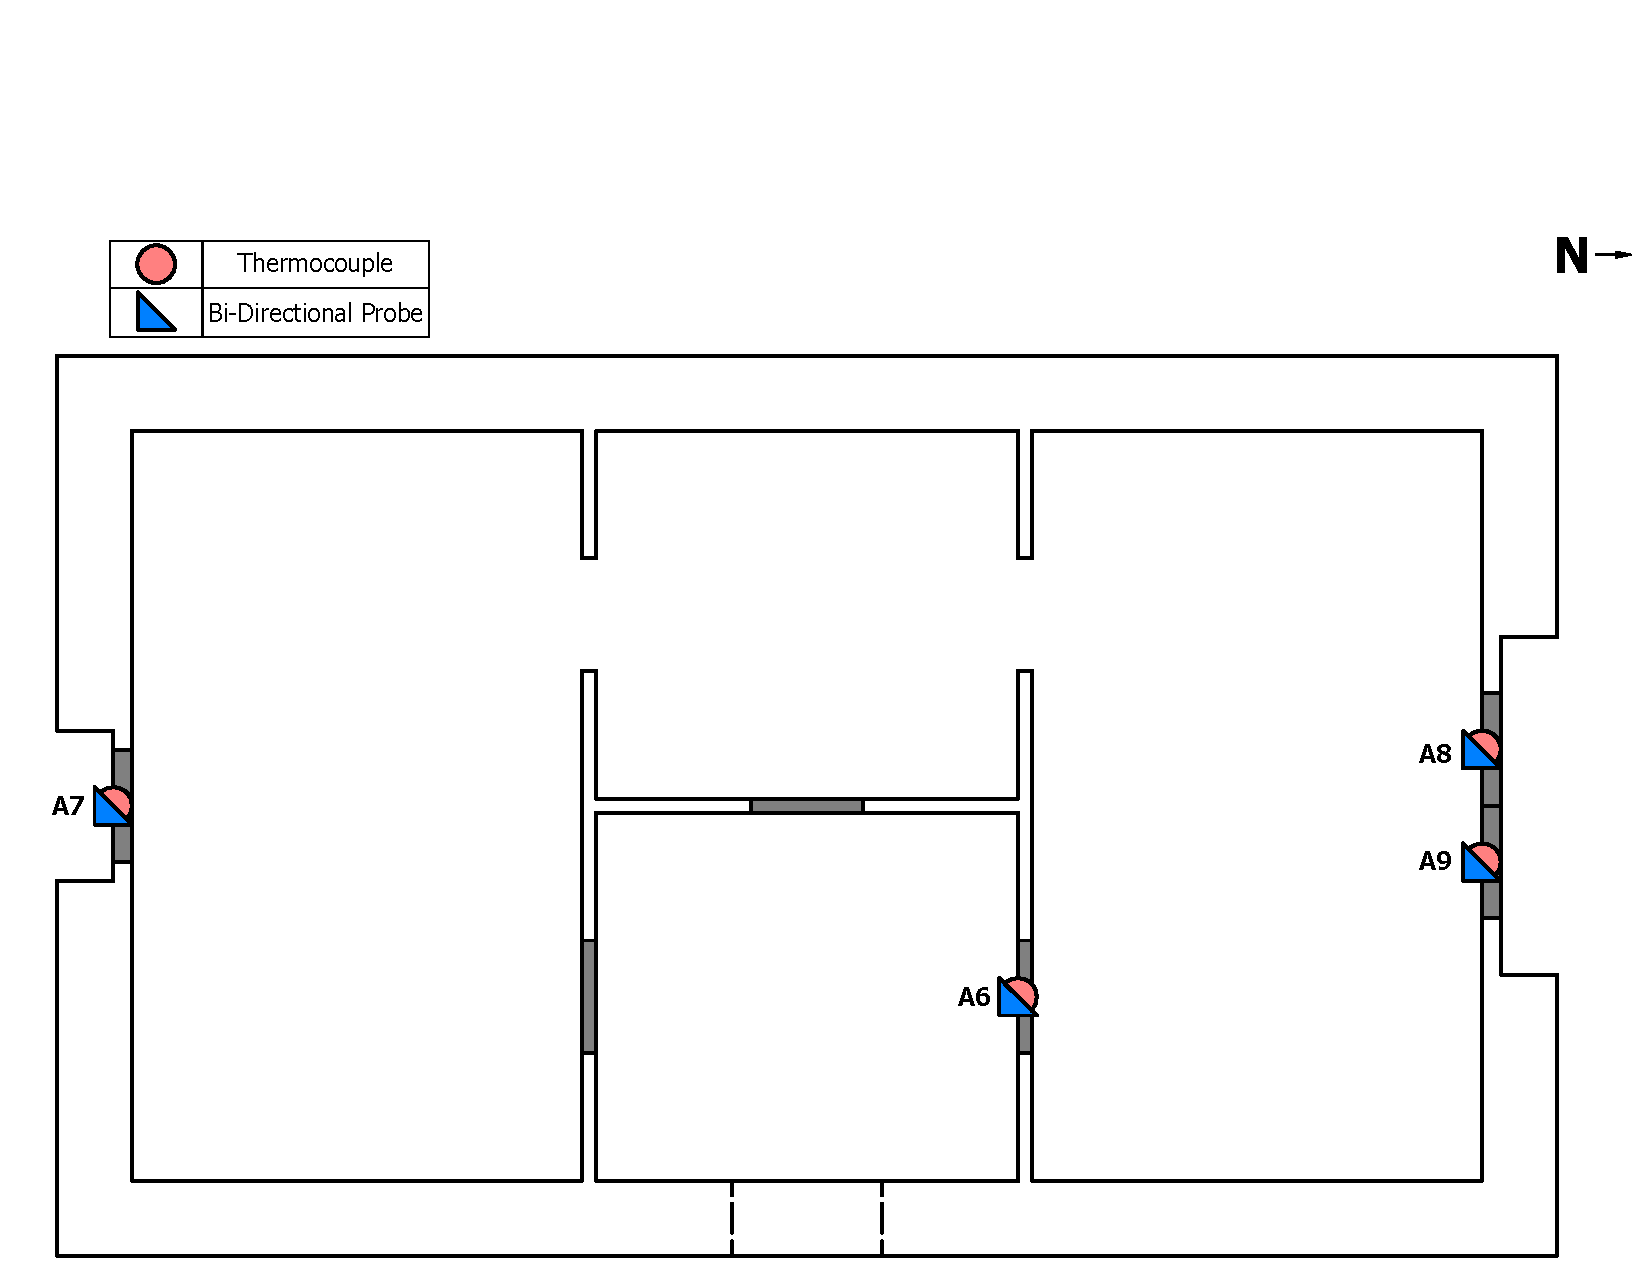
\includegraphics[trim=0cm 0cm 0.25cm 3.75cm, clip=true, width=6in]{../Drawings/Instrumentation/East_Structure_Devices_Hose_Test}
\caption[Location of Instrumentation in East Structure]{Location of instrumentation in East Structure}
\label{fig:east_instrumentation}
\end{figure}

\begin{figure}[!ht]
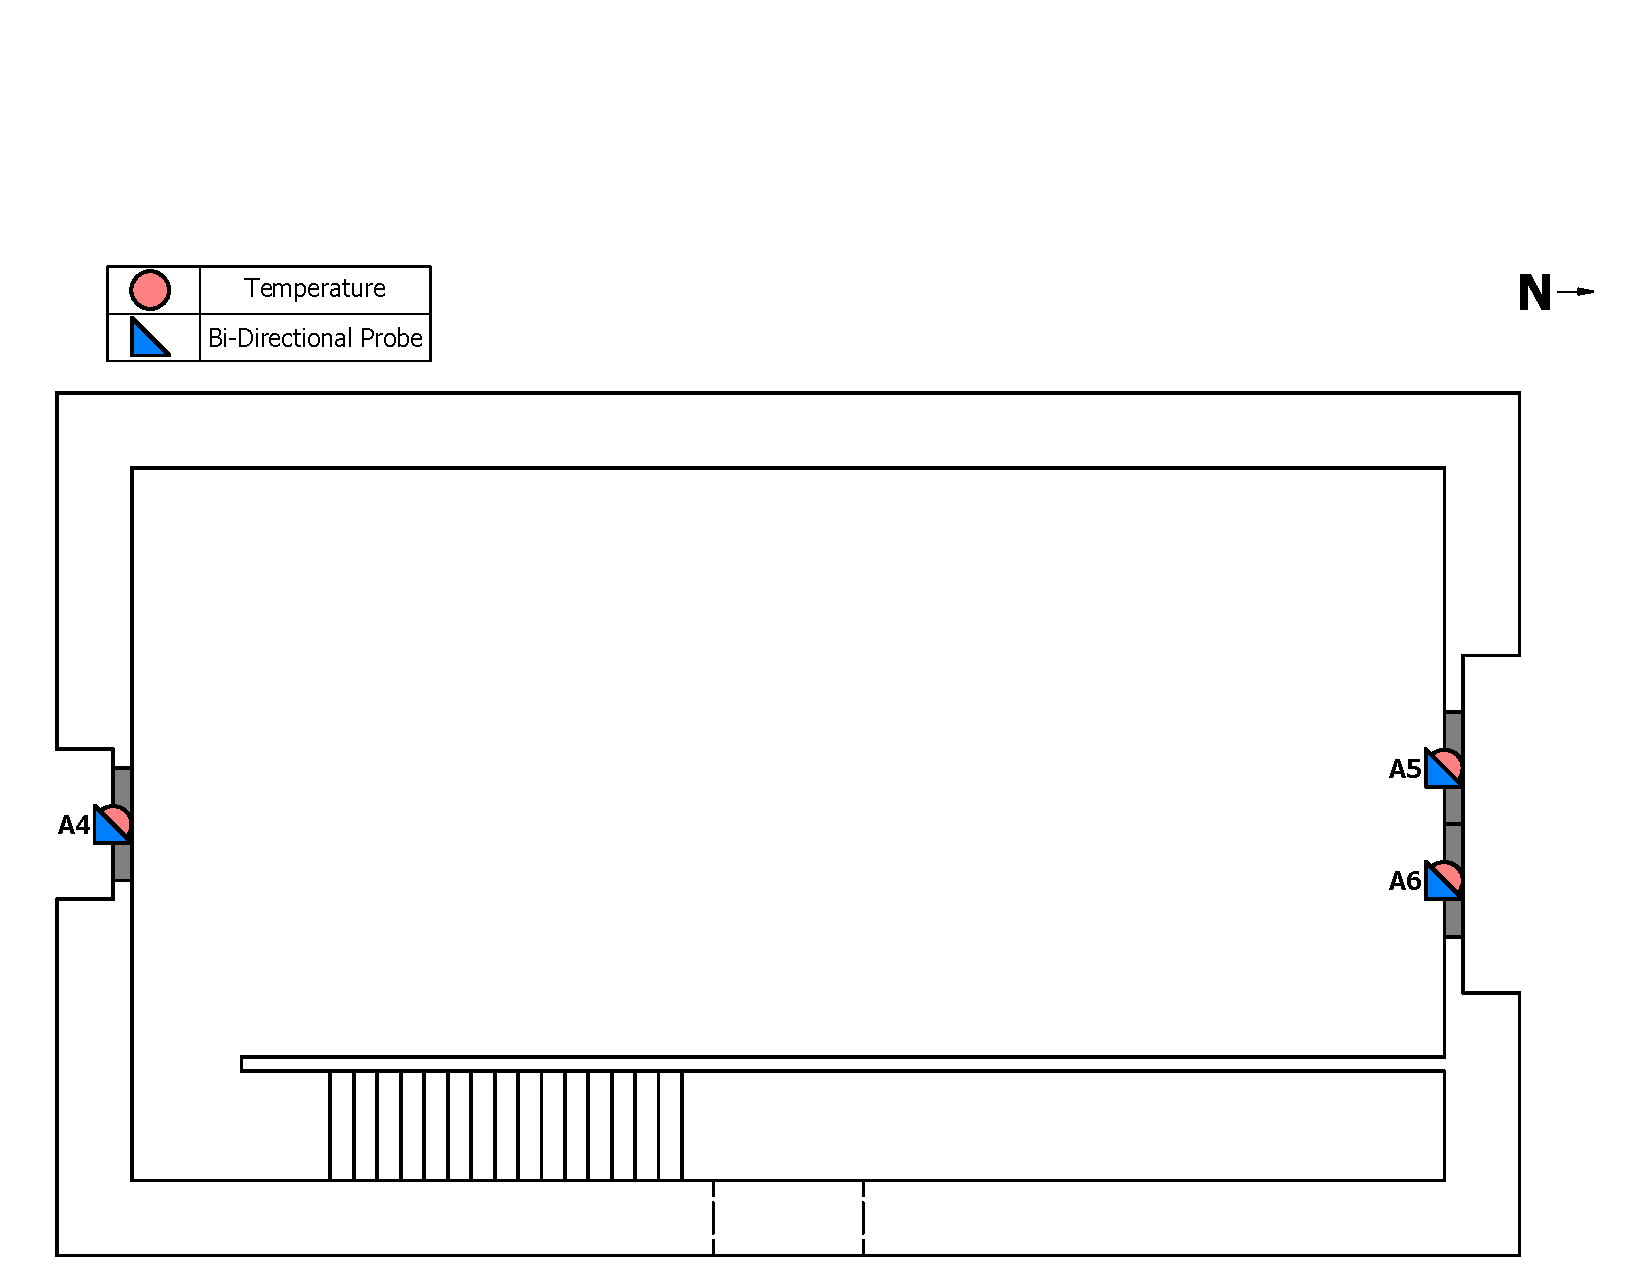
\includegraphics[trim=0cm 0cm 0.75cm 4.5cm, clip=true, width=6in]{../Drawings/Instrumentation/West_Test_Structure_Devices_Hose_Test_1st_Floor}
\\
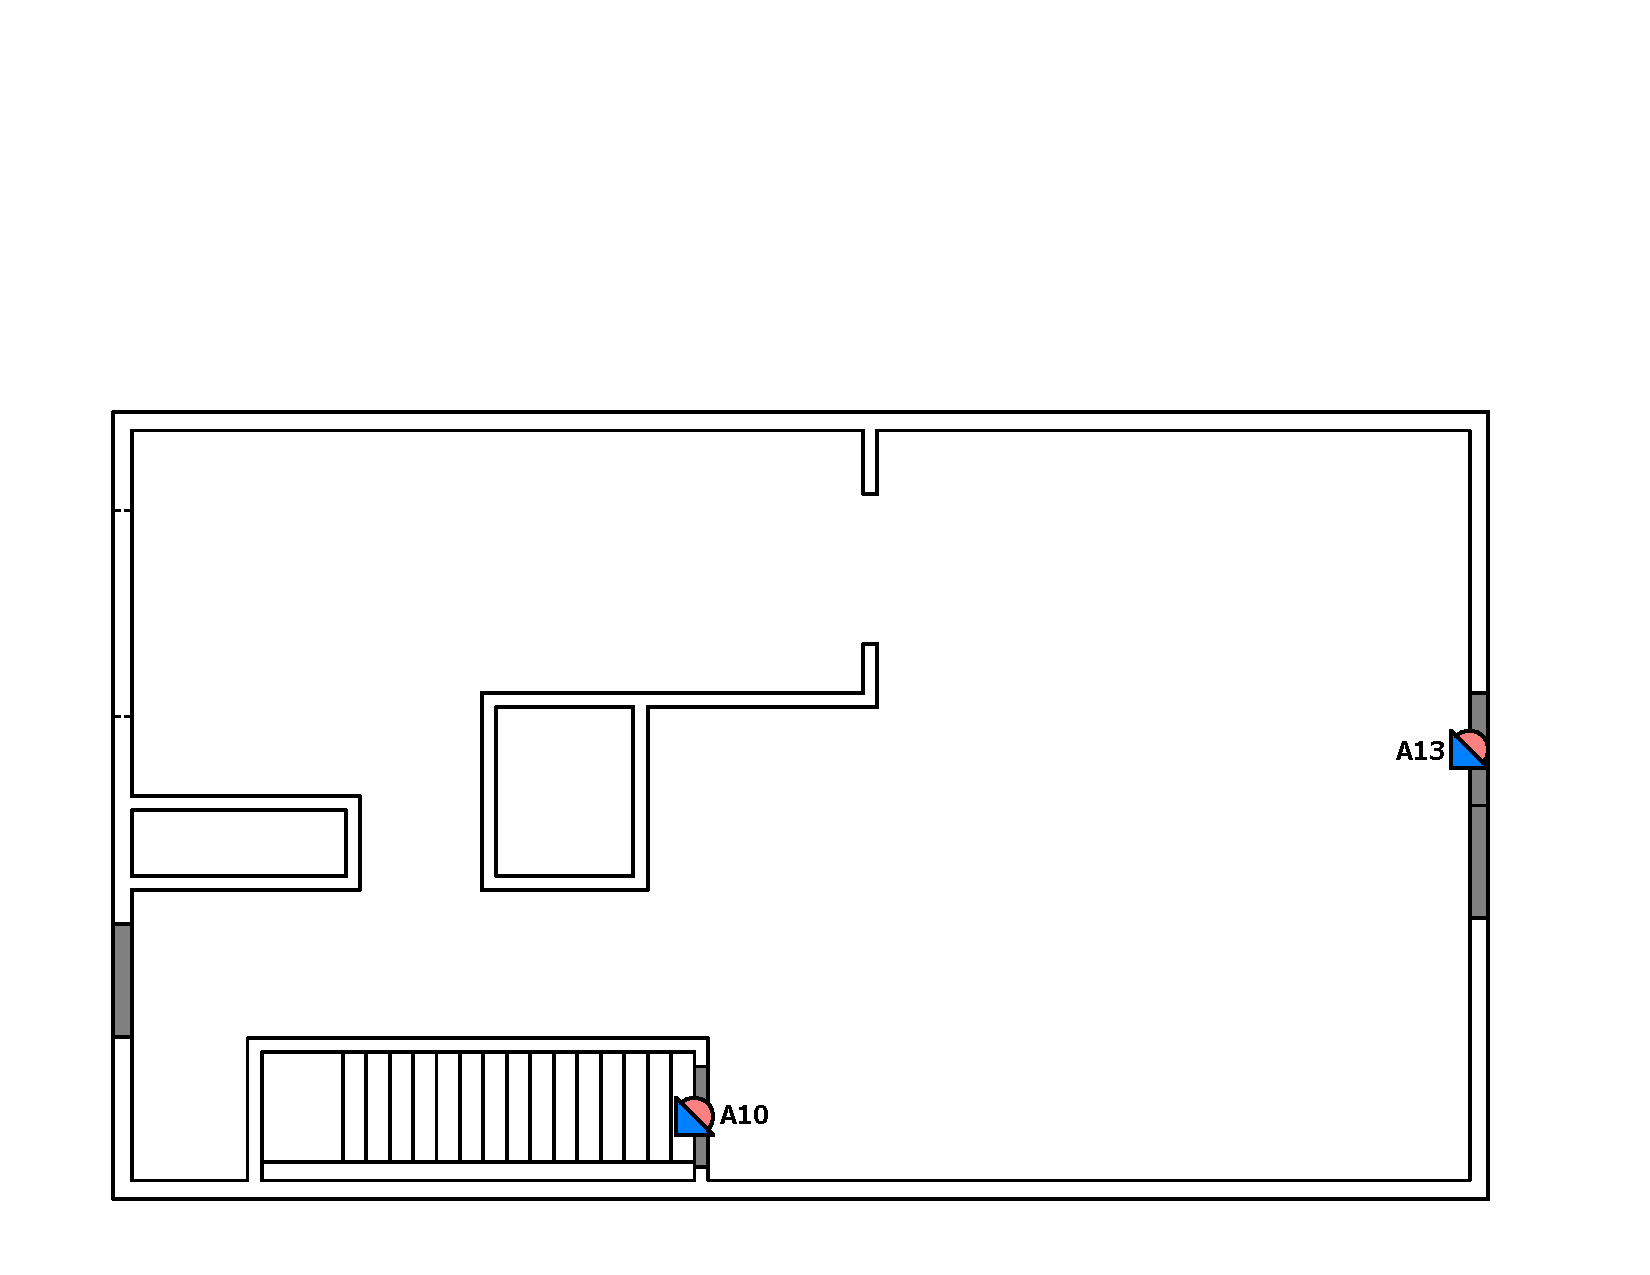
\includegraphics[trim=0cm 0cm 0.75cm 5.0cm, clip=true, width=6in]{../Drawings/Instrumentation/West_Test_Structure_Devices_Hose_Test_2nd_Floor}
\caption[Location of Instrumentation in West Structure]{Location of instrumentation in West Structure}
\label{fig:west_instrumentation}
\end{figure}

\clearpage

\begin{figure}[!ht]
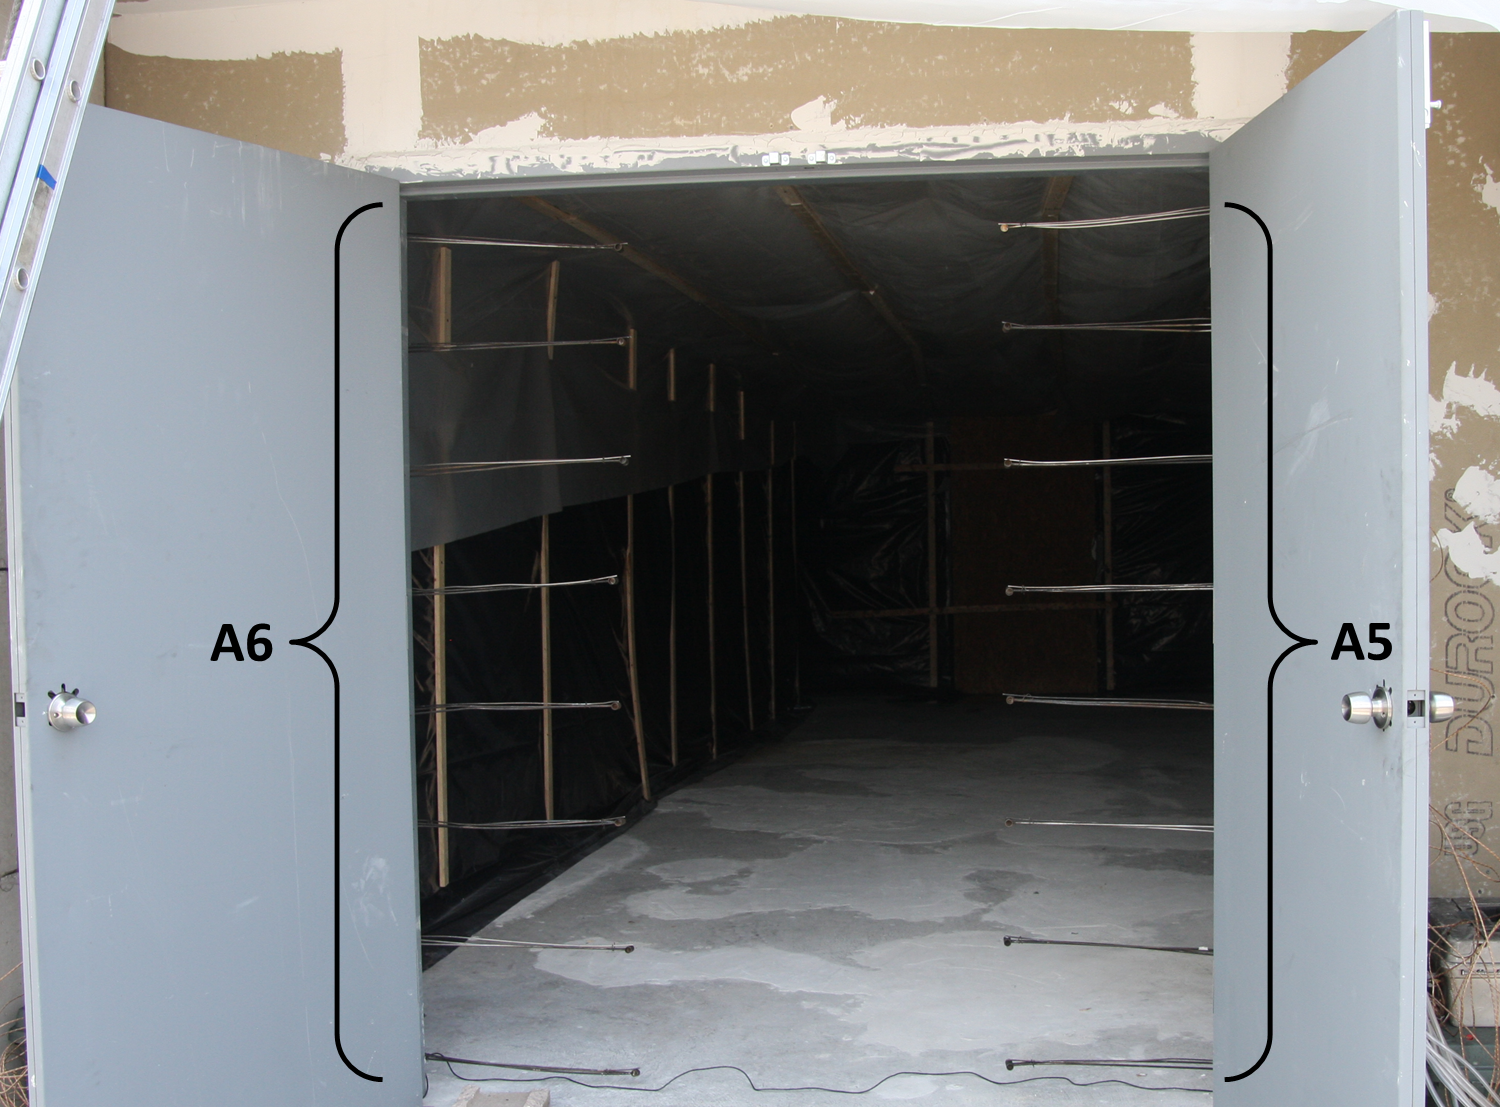
\includegraphics[width=6in]{../Pictures/BDPs}
\caption[Two sets of BDPs in Doorway of West Structure]{Two sets of BDPs, A5 and A6, in each doorway of the double doors on the first floor of the West Structure}
\label{fig:BDPs}
\end{figure}

\section{Uncertainty}
\label{sec:Uncertainty}
There are different components of uncertainty in the length, differential pressure, and gas velocity reported here. Uncertainties are grouped into two categories according to the method used to estimate them. Type A uncertainties are those which are evaluated by statistical methods, and Type B are those which are evaluated by other means~\cite{Taylor&Kuyatt:1994}. Type B analysis of systematic uncertainties involves estimating the upper (+a) and lower (-a) limits for the quantity in question such that the probability that the value would be in the interval ($\pm$a) is essentially 100\%. After estimating uncertainties by either Type A or B analysis, the uncertainties are combined in quadrature to yield the combined standard uncertainty. Then, the combined standard uncertainty is multiplied by a coverage factor of two, which results in the expanded uncertainty with a 95\% confidence interval (2$\sigma$). For some of these components, such as the zero and calibration elements, uncertainties are derived from referenced instrument specifications. For other components, referenced research results and past experience with the instruments provided input in the uncertainty determination. 

Each length measurement was taken carefully. Length measurements such as the room dimensions,
instrumentation array locations, and fire apparatus (for example nozzle, sprinkler, or fan) placement were made with a hand held laser measurement device which is has an accuracy of $\pm6.0$ mm (0.24 in) over a range of 0.61 m (2.00 ft) to 15.3 m (50.0 ft)~\cite{Stanley}. However, conditions affecting the measurement, such as levelness of the device, yield an estimated uncertainty of $\pm$0.5\% for measurements in the 2.0 m (6.6 ft) to 10.0 m (32.8 ft) range. Steel measuring tapes with a resolution of $\pm$0.5 mm were used to locate individual sensors within a measurement array and to measure and position the furniture. The steel measuring tapes were manufactured in compliance with NIST Manual 44, which specifies a tolerance of $\pm1.6$ mm (0.06 in) for 9.1 m (30 ft) tapes and $\pm6.4$ mm (0.25 in) for 30.5 m (100 ft) tapes \cite{NIST_Manual_44}. Some issues, such as "soft" edges on the upholstered furniture, result in an estimated total expanded uncertainty of $\pm$1.0\%. 

Bi-directional probes and single thermocouples were used to measure the velocity. The bi-directional probes used similar pressure transducers as those used for the differential pressure measurements discussed above. Bare-bead Type K thermocouple are co-located with the probe. A gas velocity measurement study, examining the doorway flow of pre-flashover compartment fires, yielded expanded uncertainty measurements ranging from $\pm0.14$ to $\pm0.22$ for bi-directional probes of similar design \cite{Bryant:FSJ2009}. The total expanded uncertainty for gas velocity in these experiments estimated to be $\pm18$\%.   

Water flowrate was measured with a pressure and flow meter combination shown in Fig. \ref{fig:flow_meter}. The meter consists of a section of 6.35 cm (2.5 inch) cast aluminum pipe with a 0-4.1 MPa (0-600 psi) pressure transducer and a paddlewheel type flow sensor with a range of 0 to 4800 lpm (1250 gpm). The pressure transducer and paddlewheel both connect to the battery operated control box where the pressure transducer voltage is converted to a pressure and the paddlewheel pulse count is converted to a volumetric flow rate. The manufacturer reports a $\pm5$\% calibration expanded uncertainty for the flow sensor and $\pm3$\%  for the pressure sensor \cite{Akron}. The pressure transducer was calibrated with a known analog pressure gauge. The flow meter was calibrated by capturing water over time and measuring that mass of water to determine the flowrate. The total expanded uncertainty was estimated at $\pm10$\%. 

\begin{figure}[!ht]
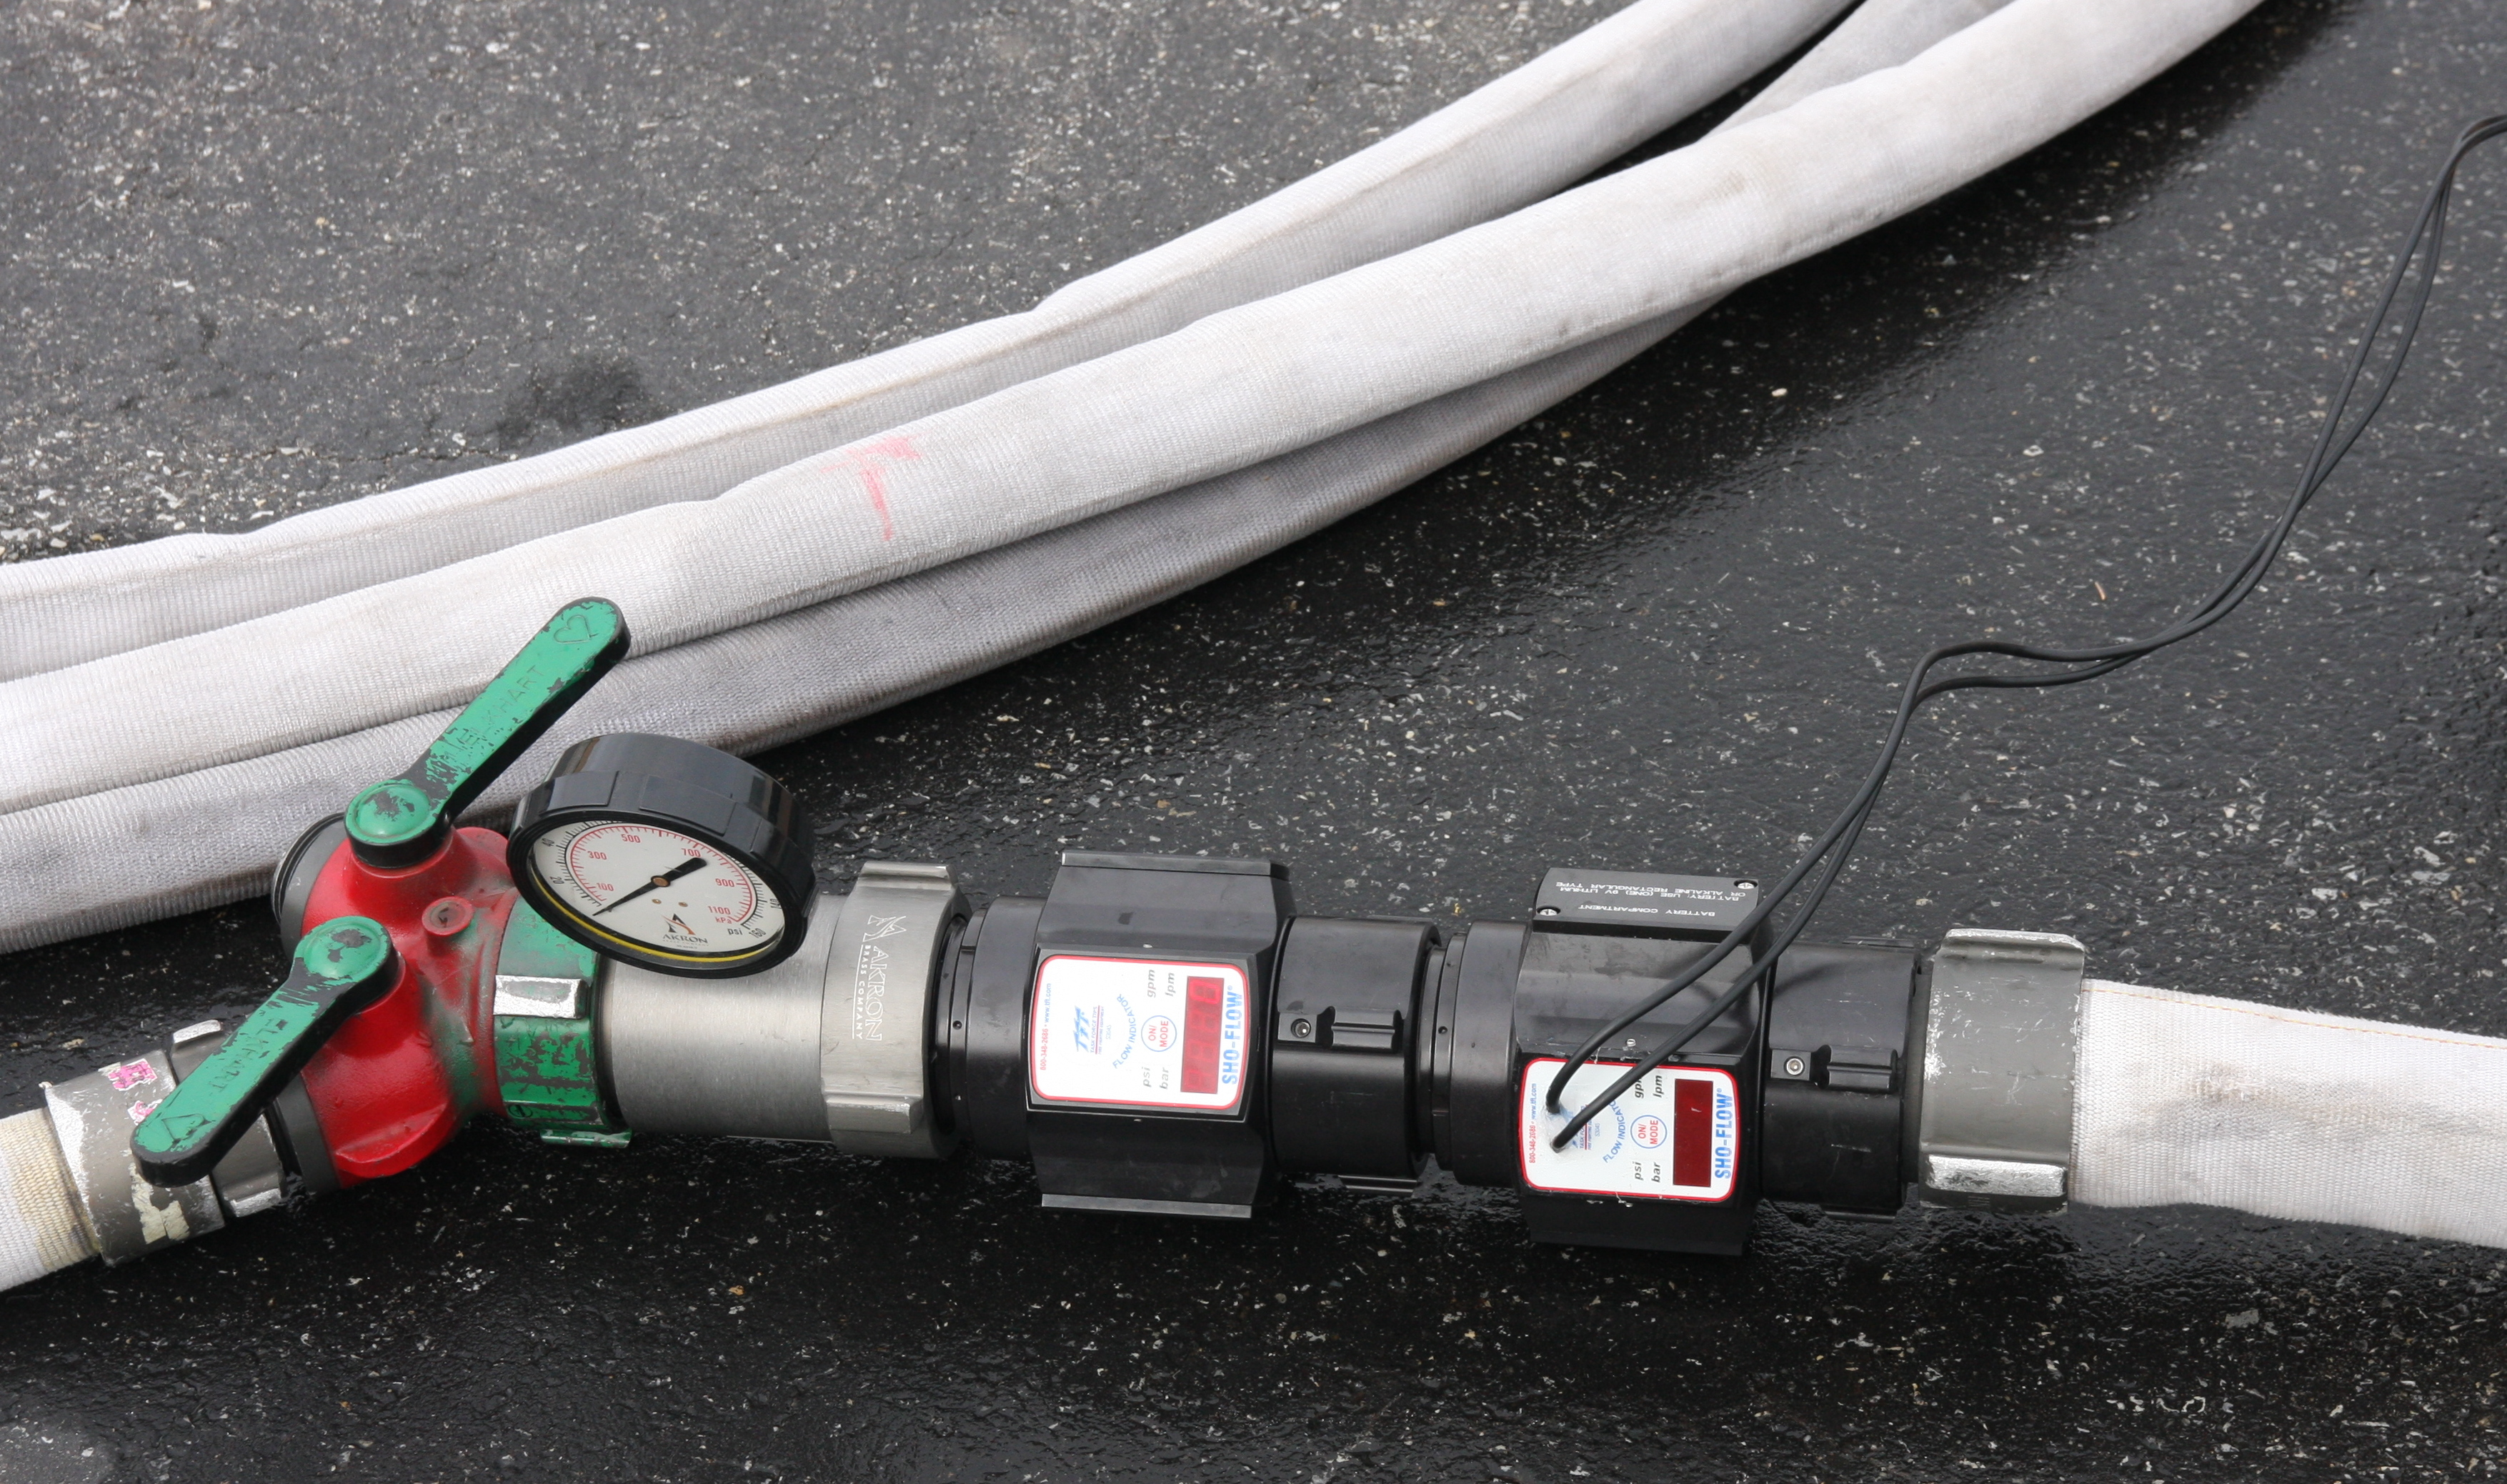
\includegraphics[width=6in]{../Pictures/flow_meter}
\caption[Picture of Flowrate Meter]{Pressure and flow meter combination used to measure water flowrate}
\label{fig:flow_meter}
\end{figure}
\FloatBarrier

In the following sections, the measurements will be presented in graphic and tabular form. In the graphs, an error bar will represent the estimated uncertainty of the measurement. In the tables, the uncertainty will be included in the table of as part of the caption.

\section{Experimental Procedure}
\label{sec:Experimental_Procedure}

\subsection{Cold Flow Experimental Procedure}
\label{sec:Cold_Flow_Procedure}

\subsection{Water Flow Experimental Procedure}
\label{sec:Water_Flow_Procedure}
A variety of experiments were conducted to examine the impact of different hose streams and application methods on air flow inside a structure. All the experiments were conducted in either the East or West Structure; used a monitor %reference for specs? 2000 LPM (500 GPM)?
or 1 \nicefrac{3}{4}" handline with a combination nozzle (Fig.~\ref{fig:monitor+handline}) to flow water in a straight, narrow fog, or wide fog stream pattern; and involved opening and closing doors in the structure to change the ventilation patterns in the structure. Experiments that used a monitor to flow water focused on varying the location of water application, while the experiments that used a handline to flow water focused on varying the pattern in which water was applied.

\begin{figure}[!ht]
\minipage{3in}
\begin{center}
	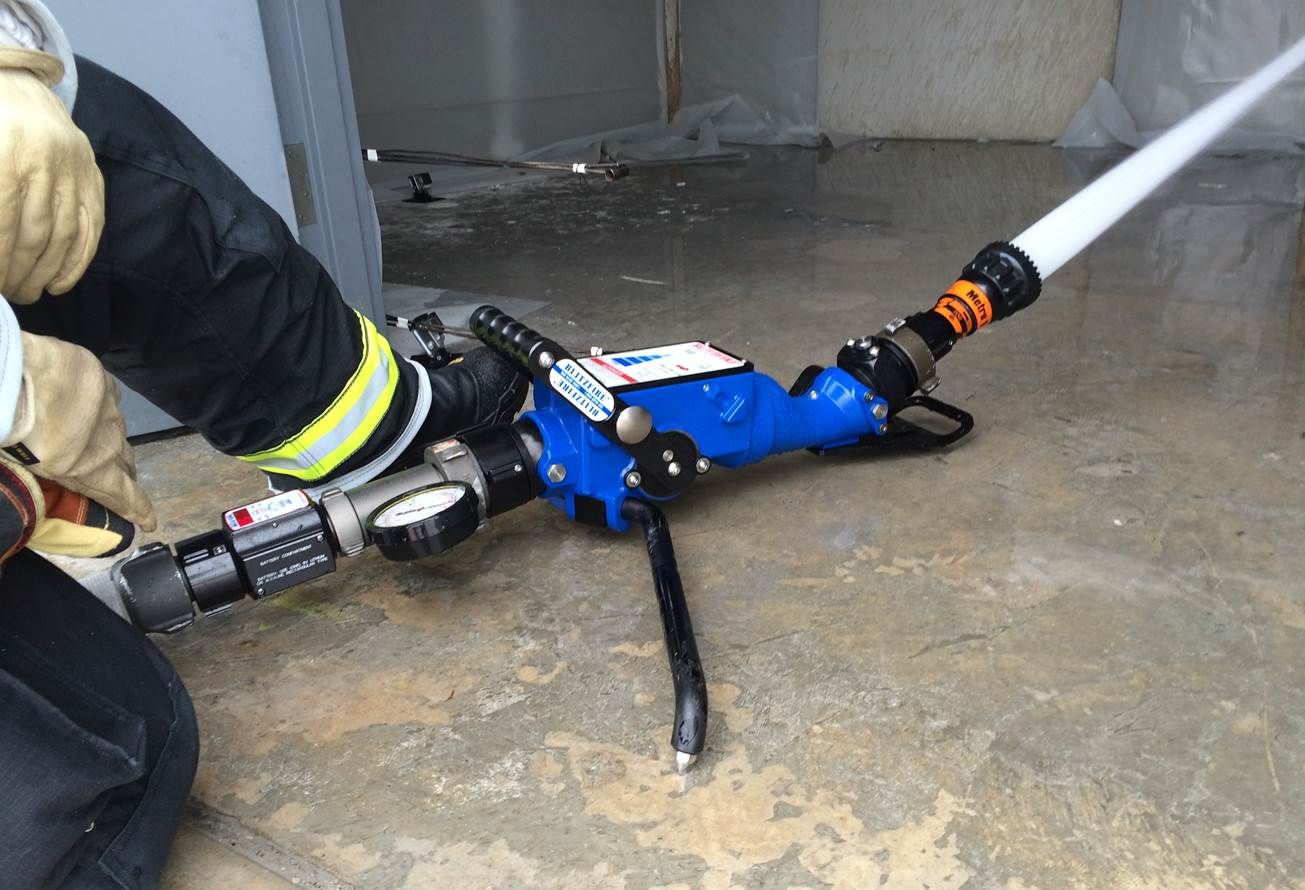
\includegraphics[width=2.9in]{../Pictures/monitor}
\end{center} 
\endminipage \hfill
\minipage{3in}
\begin{center}
	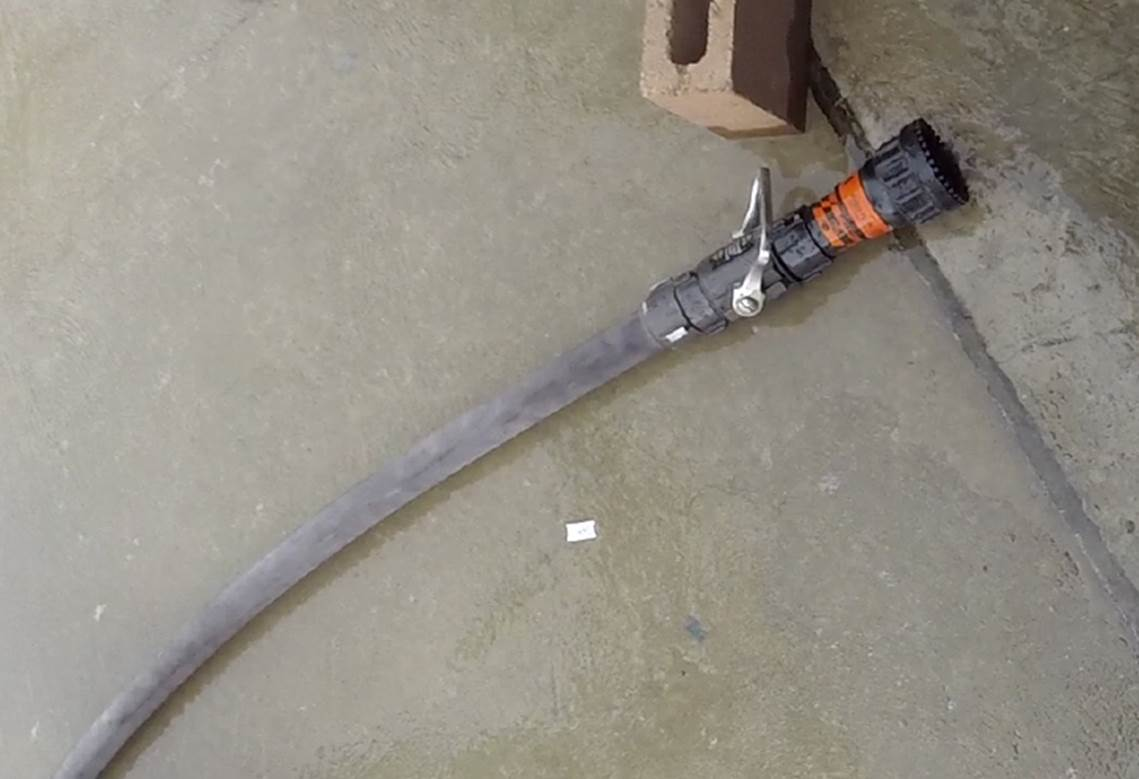
\includegraphics[width=2.9in]{../Pictures/handline}
\end{center}
\endminipage \hfill
\caption[Monitor and Handline Equipped with Combination Nozzle]{Monitor (left) and 1 \nicefrac{3}{4}" handline (right). Both are equipped with a combination nozzle and were used in the water flow experiments.}
\label{fig:monitor+handline}
\end{figure}
\FloatBarrier

\subsubsection{Monitor Experiments}
\label{sec:Water_Flow_Monitor_Procedure}
A total of five sets of experiments were conducted using a monitor with a combination nozzle to flow water. Three of the tests (Tests 29, 30, and 33) occurred in the East Structure and two of the tests (Tests 16 and 17) occurred in the West Structure. 

Tests 29 and 30 followed an identical procedure that involved flowing water from the north side double doors of the East Structure using a monitor equipped with a combination nozzle. A schematic of the structure's layout during the two tests is presented in Fig.~\ref{fig:test_29-32_setup}. Each test began by flowing water with the nozzle aimed at the ceiling of Room C, as pictured in Fig.~\ref{fig:test_29_30_pic}. After 30 seconds had elapsed, the south side door was opened for 30 seconds and then closed, and the water flow was stopped. The monitor was adjusted so the nozzle was aimed at Door BC. Then, water flow began and after 30 seconds had elapsed, the south side door was opened for 30 seconds and then closed and the water flow was stopped. This entire procedure was repeated an additional time. A straight stream pattern was used during Test 29 and a narrow fog stream pattern was used during Test 30. 

\begin{figure}[!ht]
\begin{overpic}[trim=0cm 0cm 0cm 4.5cm, clip=true, width=6in]{../Drawings/Specific_Tests/East_Structure_Hose_Test_29-32}
	\put(83,24){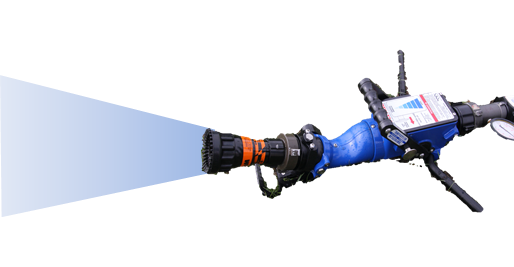
\includegraphics[width=1in]{../Drawings/monitor_graphic}}
\end{overpic}
\caption[East Structure Layout for Tests 29-32]{East Structure layout for Tests 29-32}
\label{fig:test_29-32_setup}
\end{figure}
\FloatBarrier

\begin{figure}[!ht]
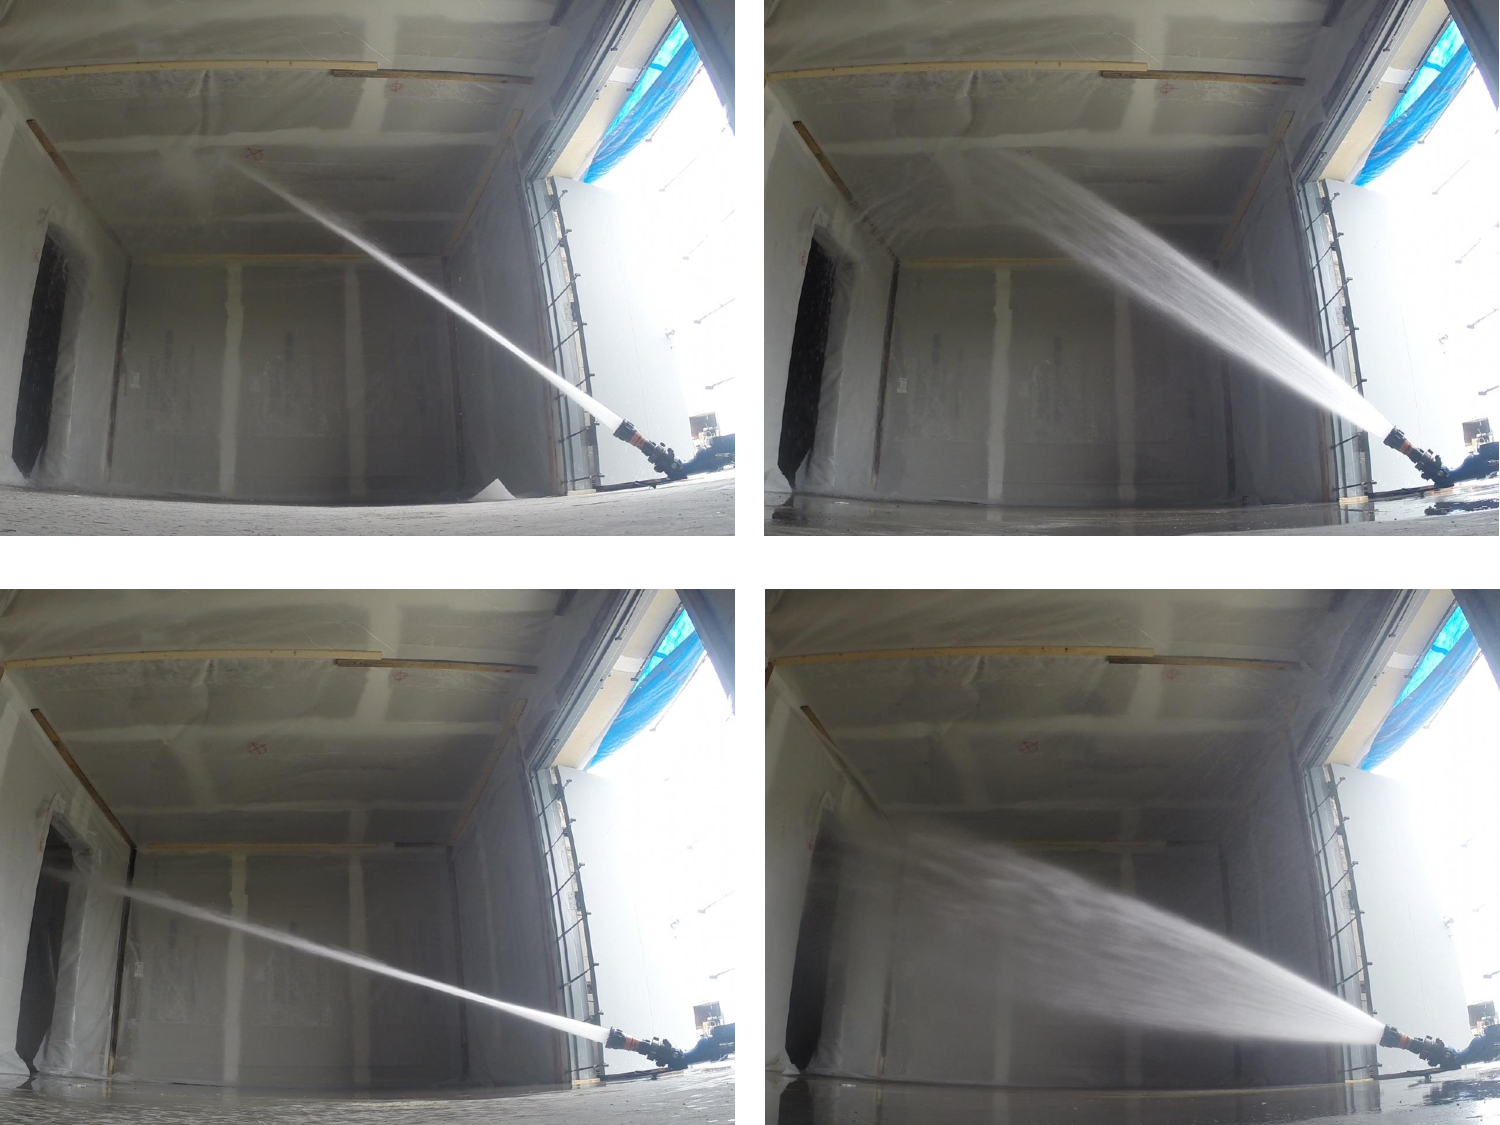
\includegraphics[width=6in]{../Pictures/East_monitor_C_BC.pdf}
\caption[Straight Stream and Narrow Fog Stream during Tests 29 and 30]{Straight stream (left column) and narrow fog stream (right column) aimed at ceiling of Room C (top row) and at Door BC (bottom row) during Tests 29 and 30}
\label{fig:test_29_30_pic}
\end{figure}
\FloatBarrier

Test 33 varied from Tests 29 and 30 in multiple ways. During Test 33, the monitor was located inside Room C and aimed at the ceiling of Room B, as shown in Fig.~\ref{fig:test_33_pic}. A schematic of the structure's layout during Test 33 is presented in Fig.~\ref{fig:test_33_34_setup}. The test began by flowing water in a straight stream pattern for 30 seconds, then in a narrow fog stream for 30 seconds, and finally in a wide fog stream for 30 seconds. Then, the south side door was opened and each stream was applied for 30 seconds again.

\begin{figure}[!ht]
\begin{overpic}[trim=0cm 0cm 0cm 4.5cm, clip=true, width=6in]{../Drawings/Specific_Tests/East_Structure_Hose_Test_33_34}
	\put(66,36){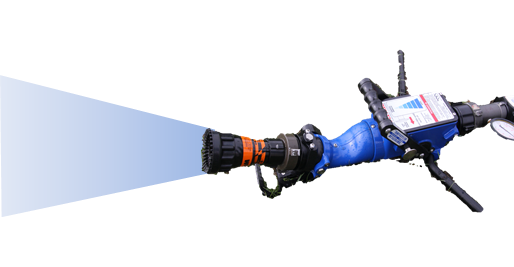
\includegraphics[width=1in]{../Drawings/monitor_graphic}}
\end{overpic}
\caption[East Structure Layout for Tests 33 and 34]{East Structure layout for Tests 33 and 34}
\label{fig:test_33_34_setup}
\end{figure}
\FloatBarrier

\begin{figure}[!ht]
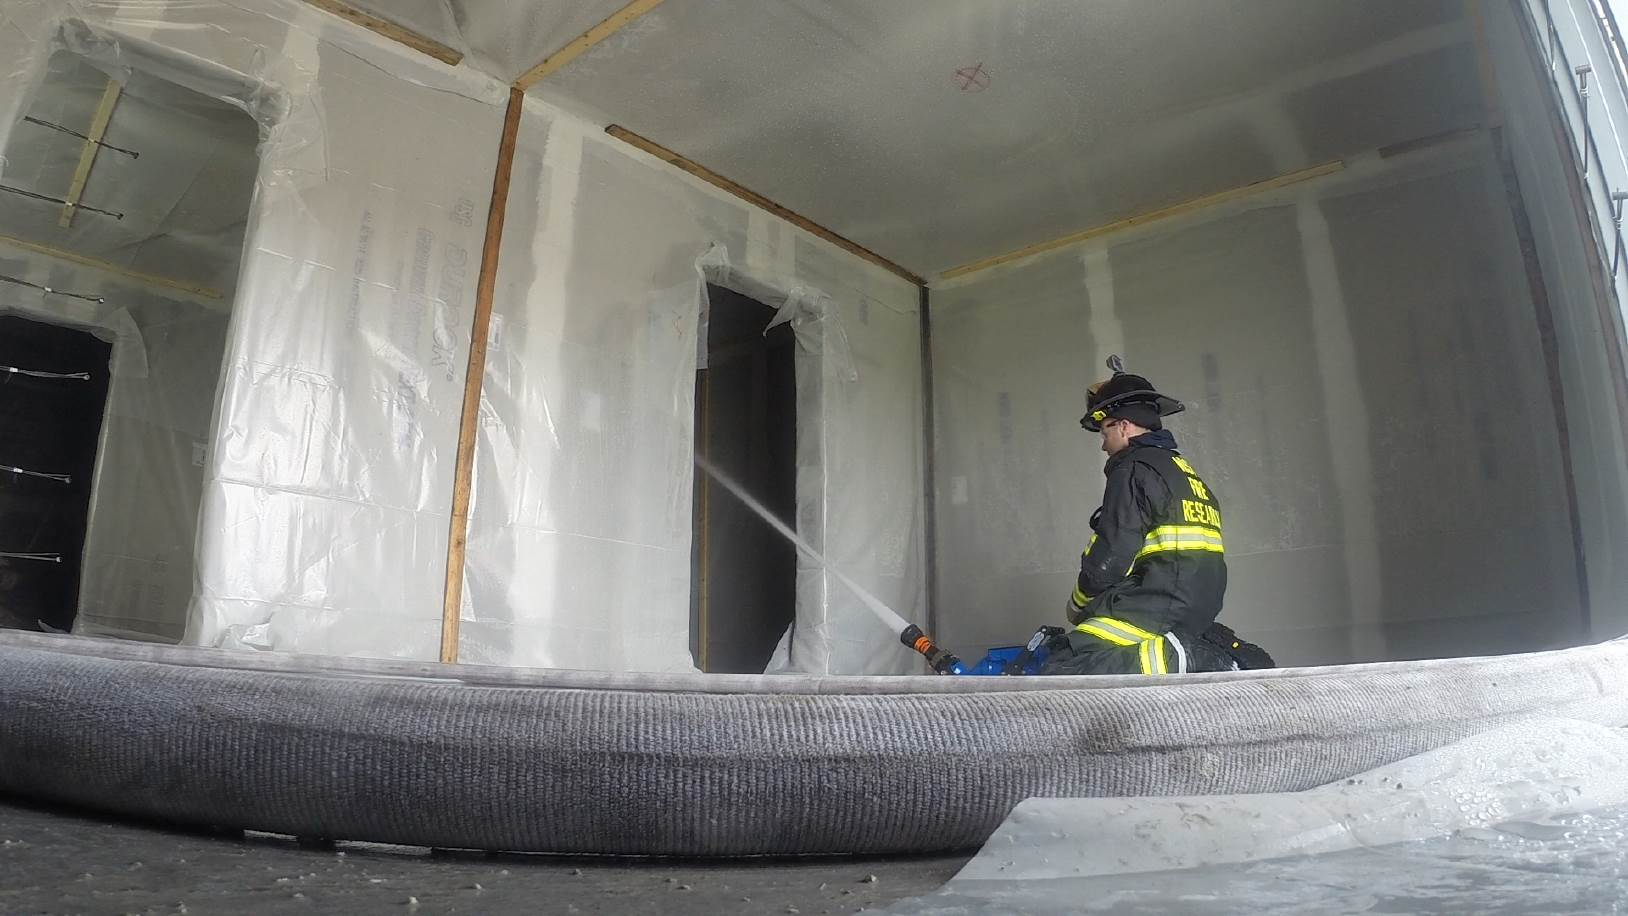
\includegraphics[trim=16cm 6.25cm 9cm 6cm, clip=true, width=4in]{../Pictures/SS_Room_B_Test_33}
\\~\\
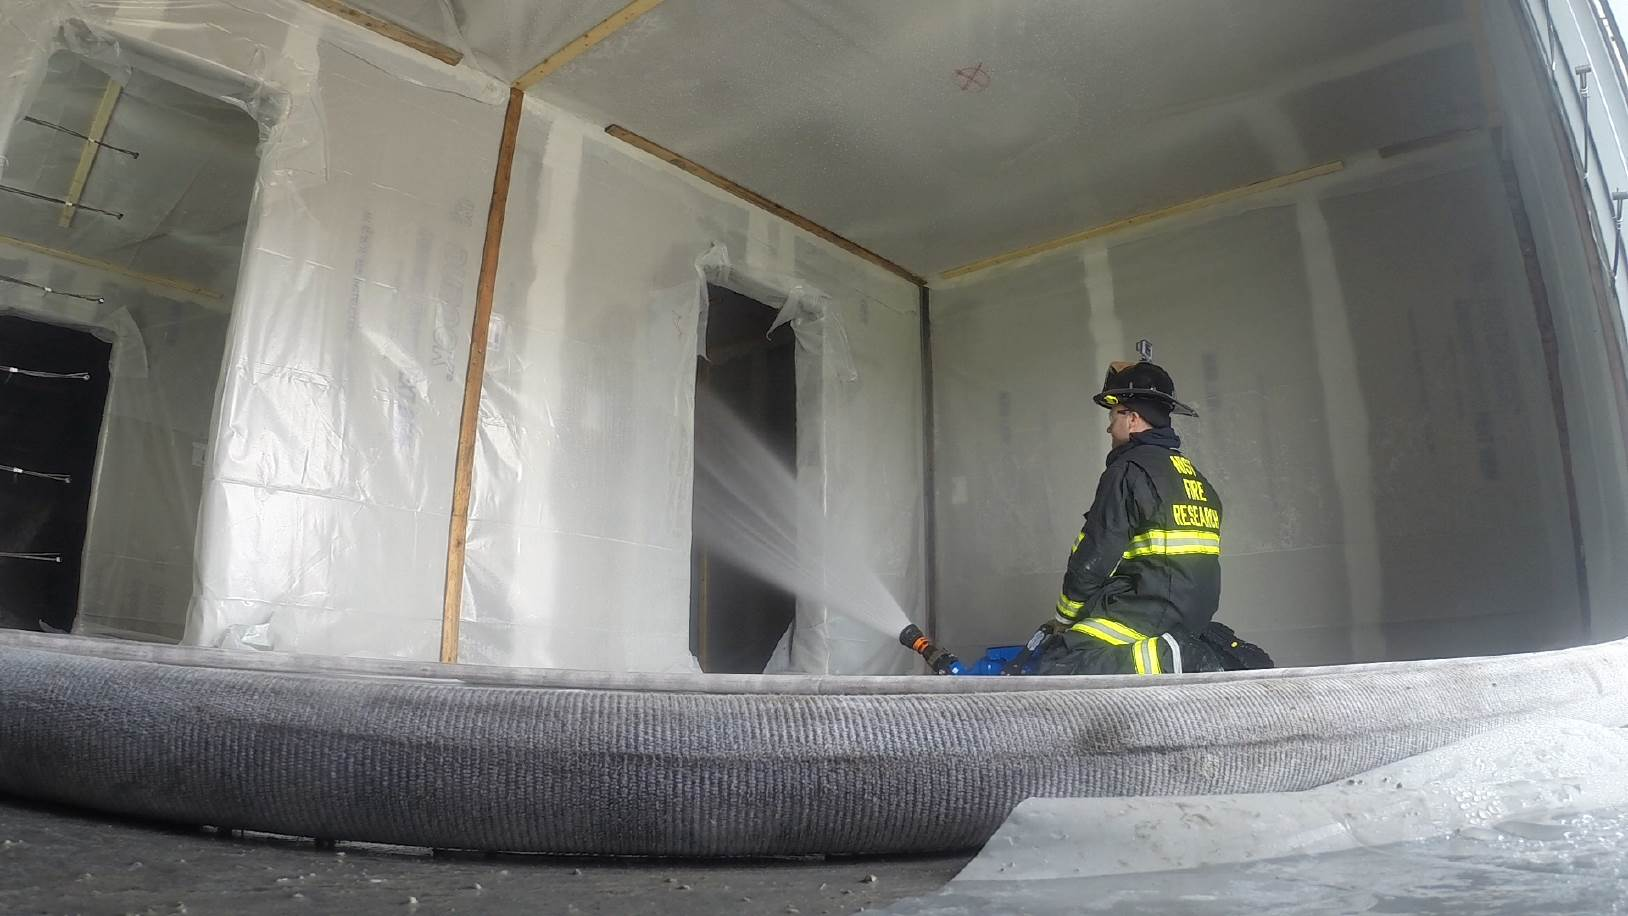
\includegraphics[trim=16cm 6.25cm 9cm 6cm, clip=true, width=4in]{../Pictures/NF_Room_B_Test_33}
\\~\\
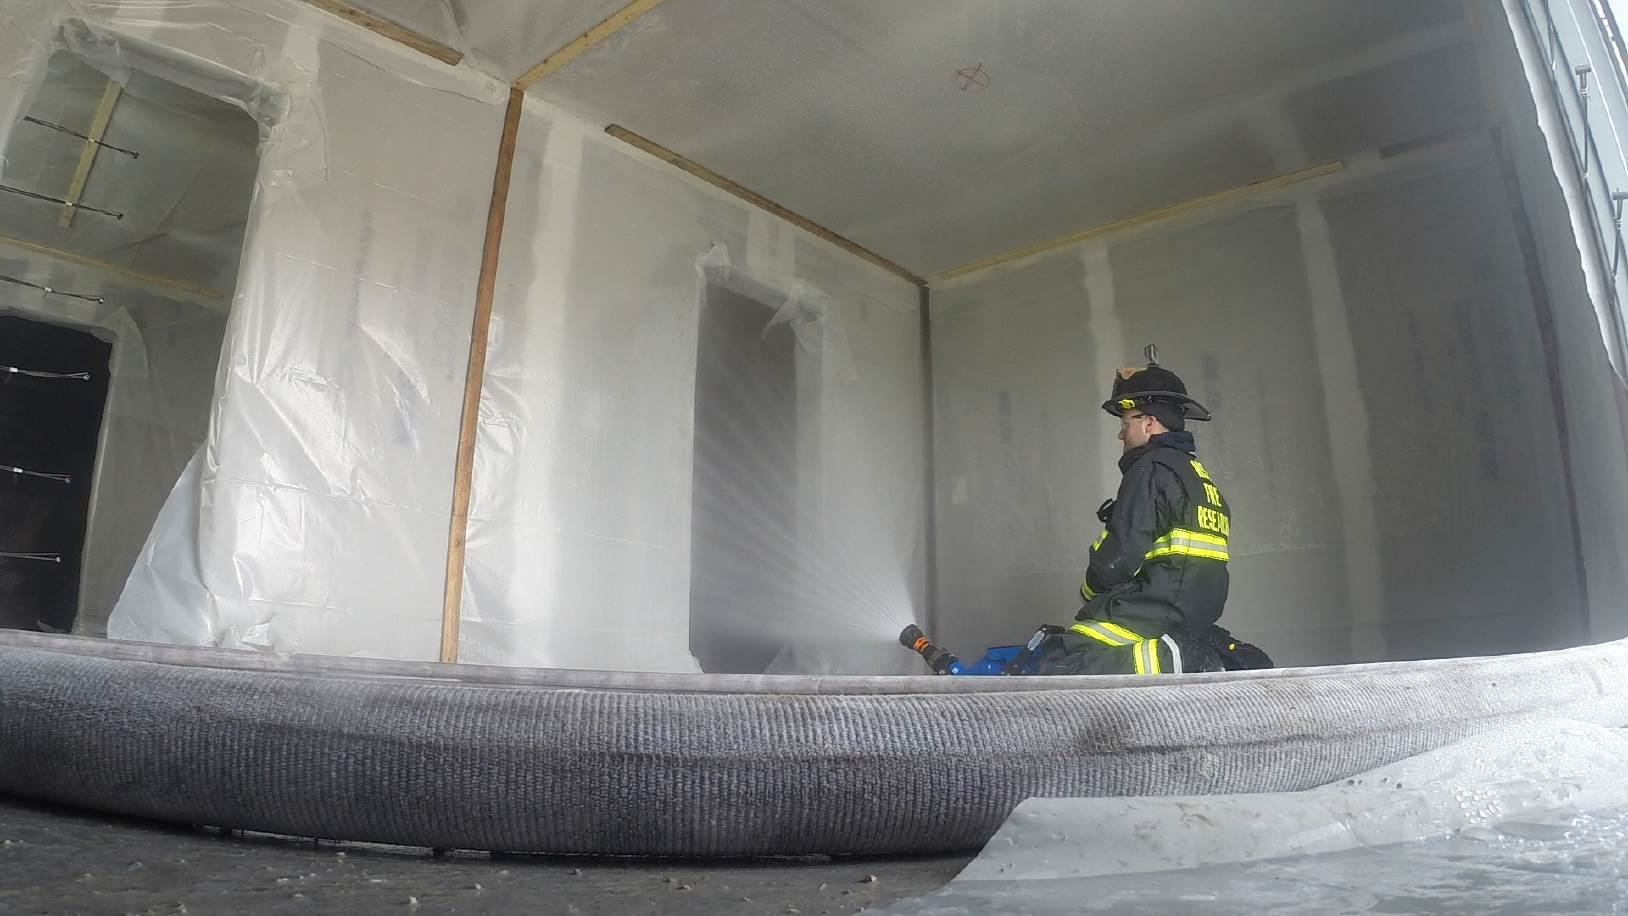
\includegraphics[trim=16cm 6.25cm 9cm 6cm, clip=true, width=4in]{../Pictures/WF_Room_B_Test_33}
\caption[Straight Stream, Narrow Fog Stream, and Wide Fog Stream during Test 33]{Straight stream (top), narrow fog stream (middle), and wide fog stream (bottom) aimed at ceiling of Room B during Test 33}
\label{fig:test_33_pic}
\end{figure}
\FloatBarrier

%ADD TARGET DIMENSION%
Tests 16 and 17 followed an identical procedure that involved flowing water from the north side double doors on the first level of the West Structure using a monitor equipped with a combination nozzle. The nozzle was aimed at two targets throughout the tests: a "near" target, located approximately X m (X ft) from the interior side of the north wall, and a "far" target, located approximately X m (X ft) from the interior side of the north wall. The difference between the tests was that Test 16 contained the flow path configuration presented in Fig.~\ref{fig:flow_path_1}, while Test 17 contained the flow path configuration presented in Fig.~\ref{fig:flow_path_2}. Each test began by flowing water in a straight stream pattern at the far target for 60 seconds. After 60 seconds of water flow, the stairwell door was opened. One minute later, the north side, west double door on the second floor was opened, and water continued to flow for 60 seconds. Then, water flow was stopped, the two doors were closed, and the procedure was repeated with the monitor aimed at the near target. The entire process was repeated for the narrow fog and wide fog streams. Fig.~\ref{fig:test_16_17_pic} contains images of each type of hose stream aimed at the near and far targets.

\begin{figure}[!ht]
\begin{overpic}[trim=0cm 0cm 0.75cm 4.5cm, clip=true, width=6in]{../Drawings/Specific_Tests/West_Structure_Hose_Test_18_1st_Floor}
	\put(81,23){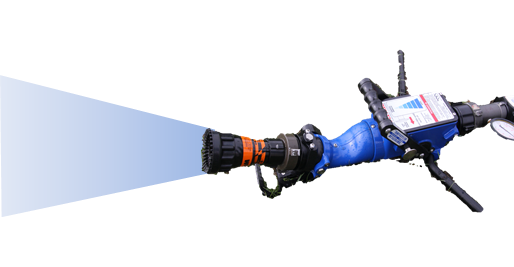
\includegraphics[width=1in]{../Drawings/monitor_graphic}}
\end{overpic}
\\
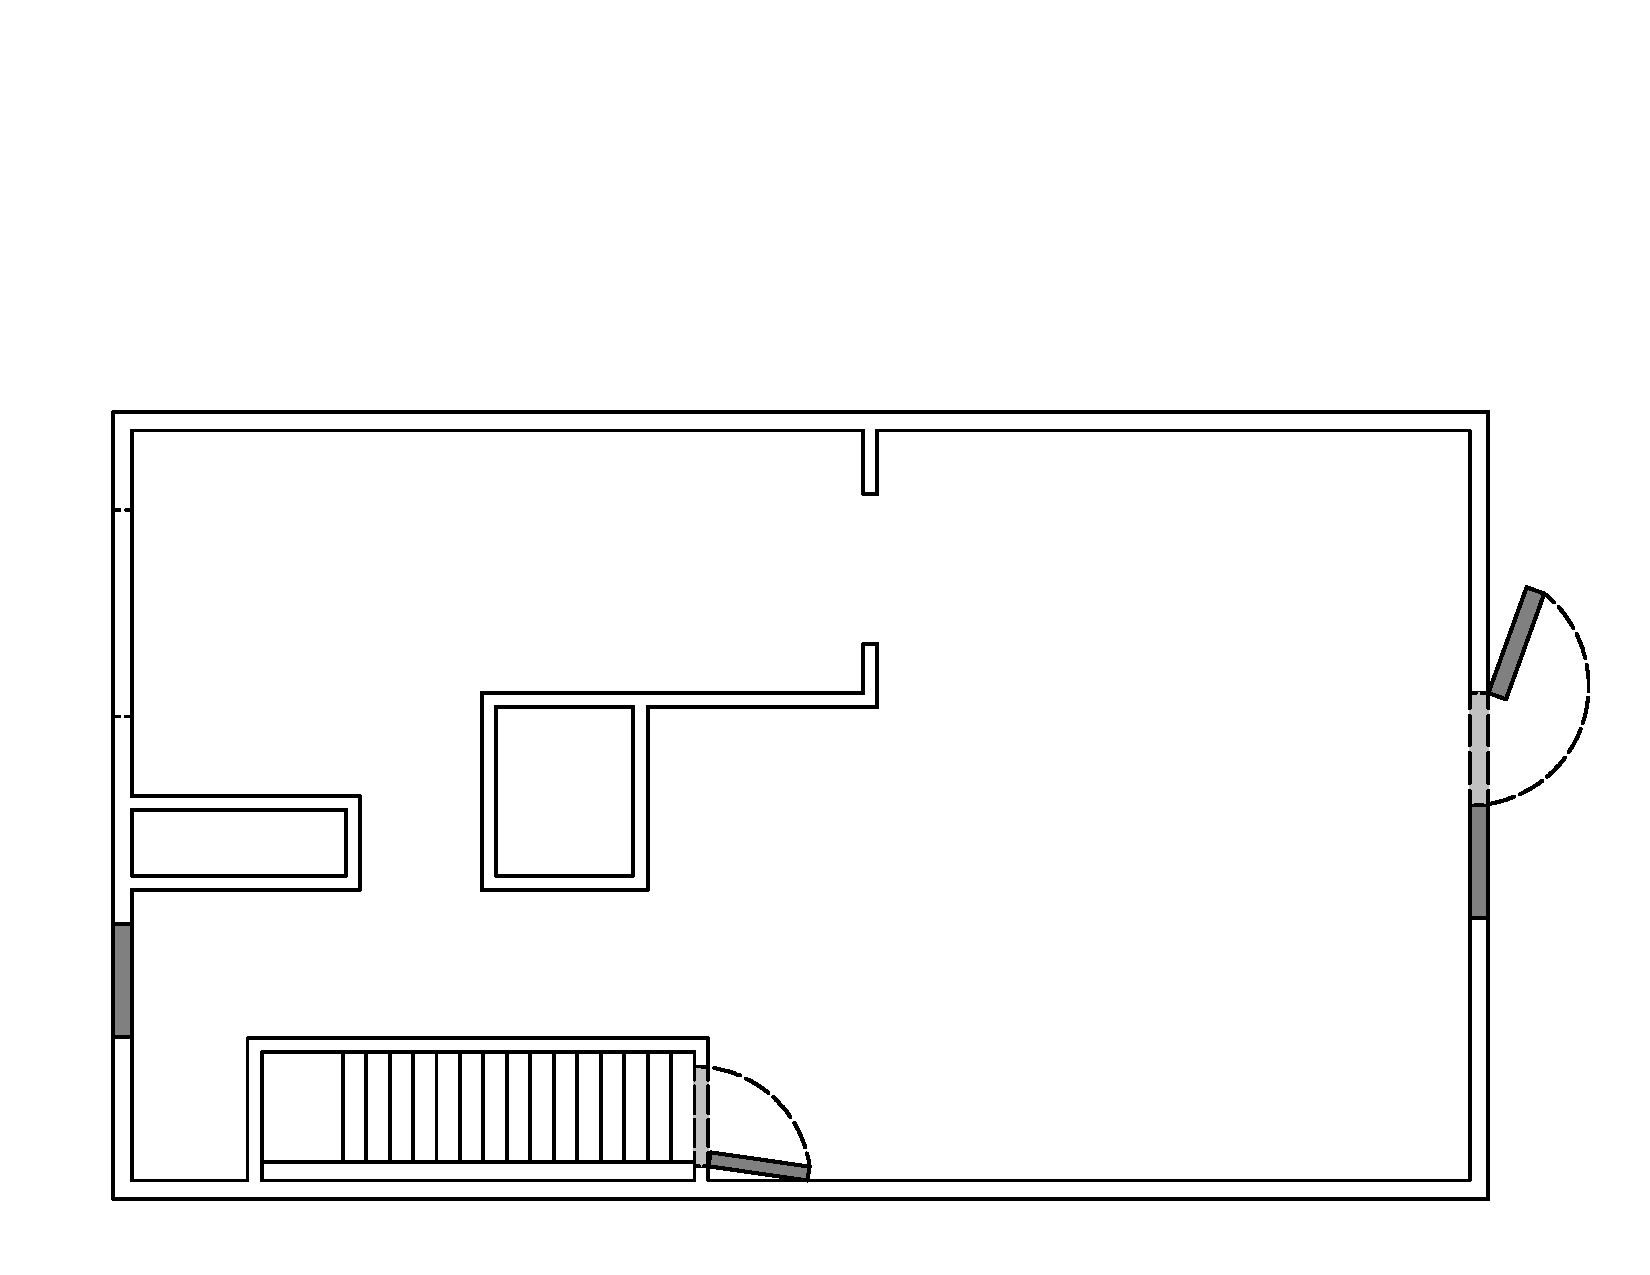
\includegraphics[trim=0cm 0cm 0.75cm 5cm, clip=true, width=6in]{../Drawings/Specific_Tests/West_Structure_Hose_Test_18_2nd_Floor}
\caption[West Structure Layout for Tests 16 and 18]{West Structure first floor (top) and second floor (bottom) layouts for Tests 16 and 18. Both double doors and the south side door on the first floor were in the opened position for the duration of the test. On the second floor, the stairwell door and north side, west double door were opened and closed during the tests, while the north side, east double door and south side door were in the closed position throughout the entire test.}
\label{fig:flow_path_1}
\end{figure}
\FloatBarrier

\begin{figure}[!ht]
\begin{overpic}[trim=0cm 0cm 0.75cm 4.5cm, clip=true, width=6in]{../Drawings/Specific_Tests/West_Structure_Hose_Test_19_1st_Floor}
	\put(81,23){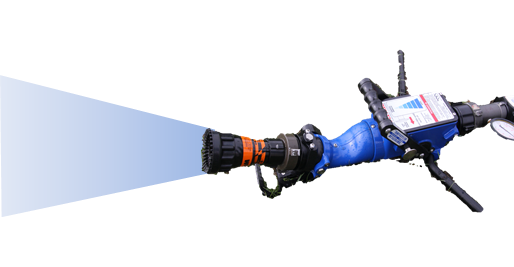
\includegraphics[width=1in]{../Drawings/monitor_graphic}}
\end{overpic}
\\
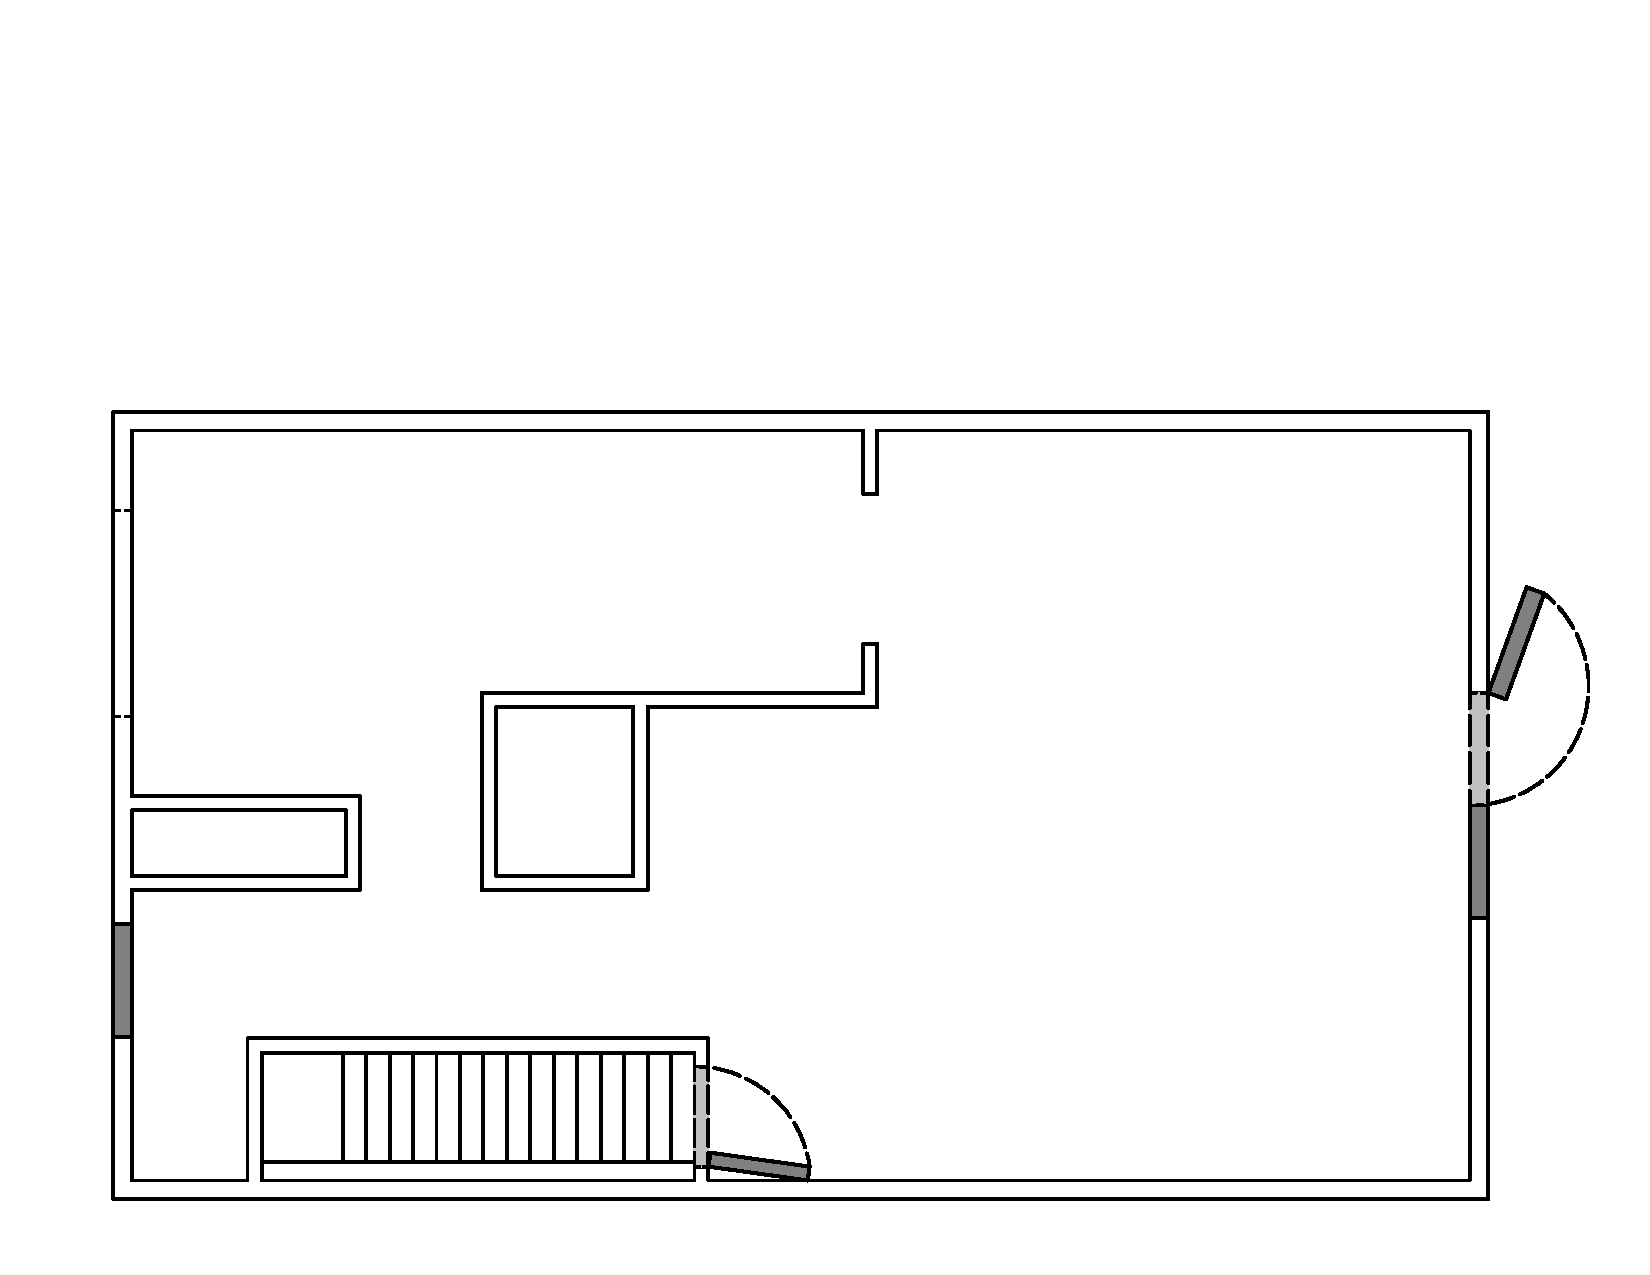
\includegraphics[trim=0cm 0cm 0.75cm 5cm, clip=true, width=6in]{../Drawings/Specific_Tests/West_Structure_Hose_Test_19_2nd_Floor}
\caption[West Structure Layout for Tests 17 and 19]{West Structure first floor (top) and second floor (bottom) layouts for Tests 17 and 19. Both double doors on the first floor were in the opened position and the south side door on the first floor was in the closed position for the duration of the test. On the second floor, the stairwell door and north side, west double door were opened and closed during the tests, while the north side, east double door and south side door were in the closed position throughout the entire test.}
\label{fig:flow_path_2}
\end{figure}
\FloatBarrier

\begin{figure}[!ht]
\minipage{2.15in}
\begin{center}
	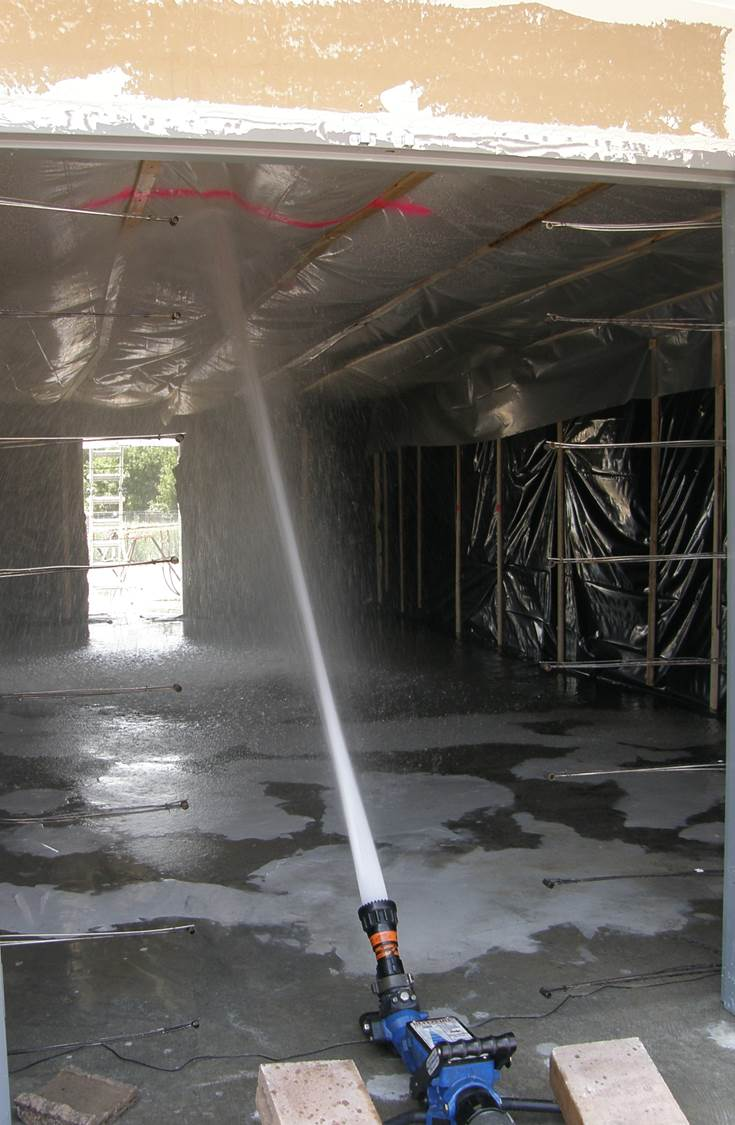
\includegraphics[width=2in]{../Pictures/SS_near}
\end{center} 
\endminipage \hfill
\minipage{2.15in}
\begin{center}
	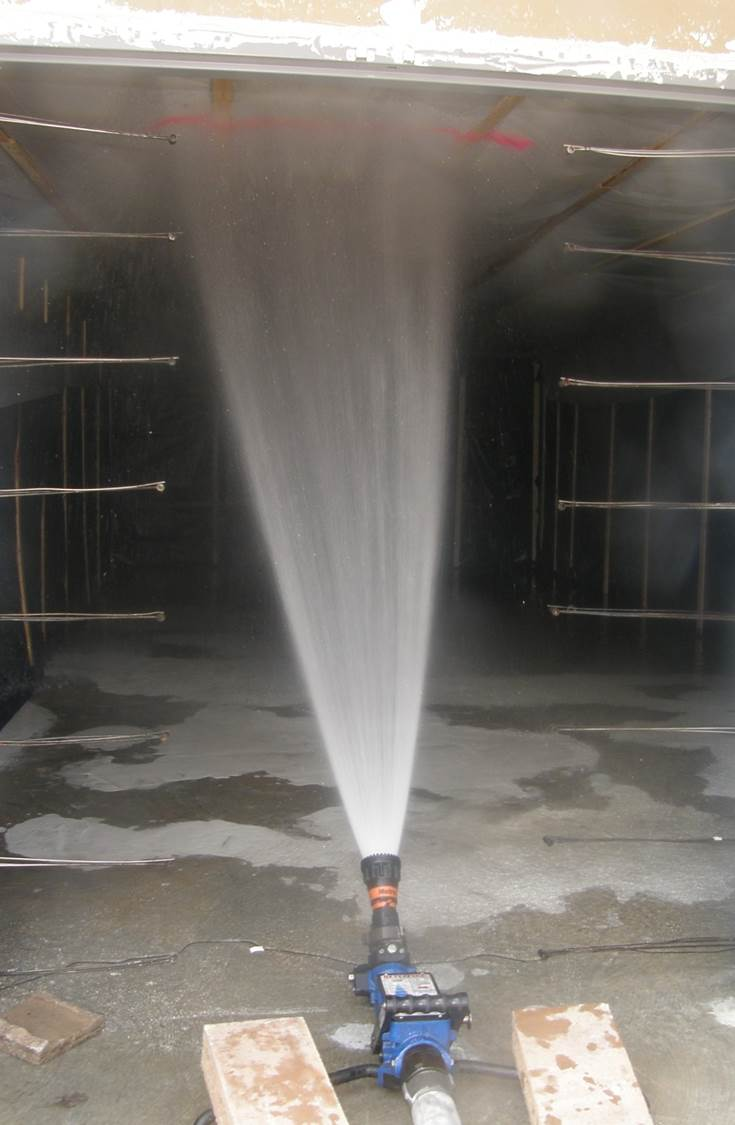
\includegraphics[width=2in]{../Pictures/NF_near}
\end{center}
\endminipage \hfill
\minipage{2.15in}
\begin{center}
	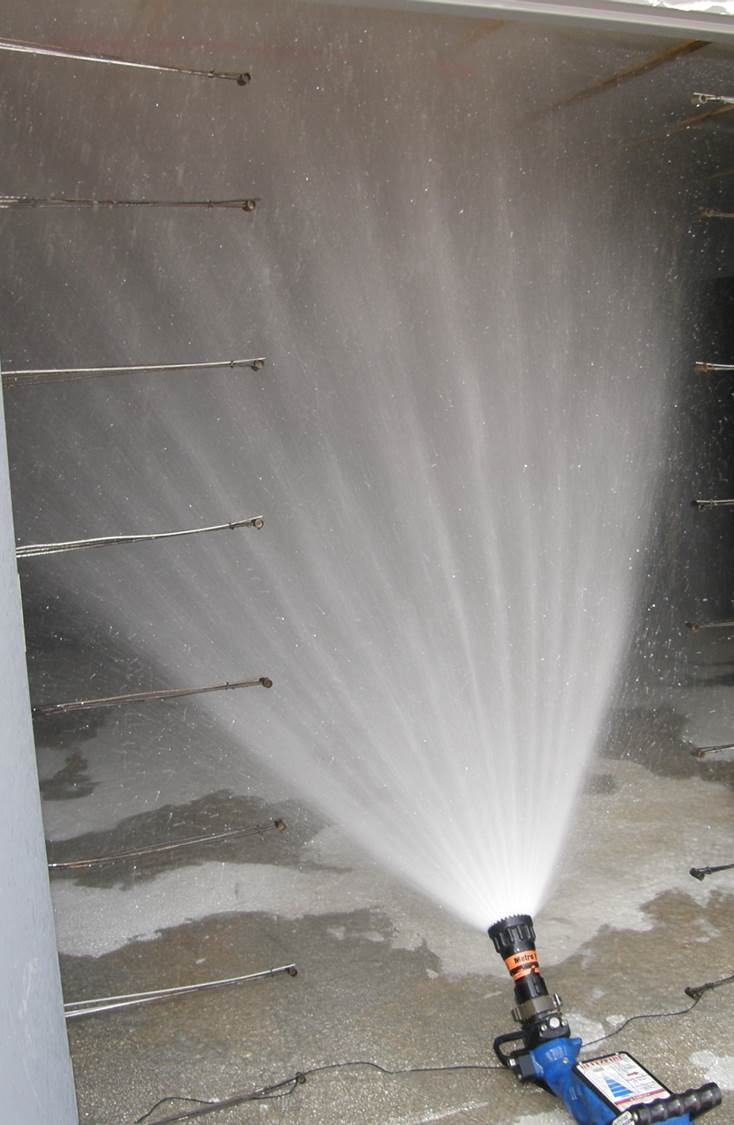
\includegraphics[width=2in]{../Pictures/WF_near}
\end{center}
\endminipage \hfill
\vspace{0.15in}
\minipage{2.15in}
\begin{center}
	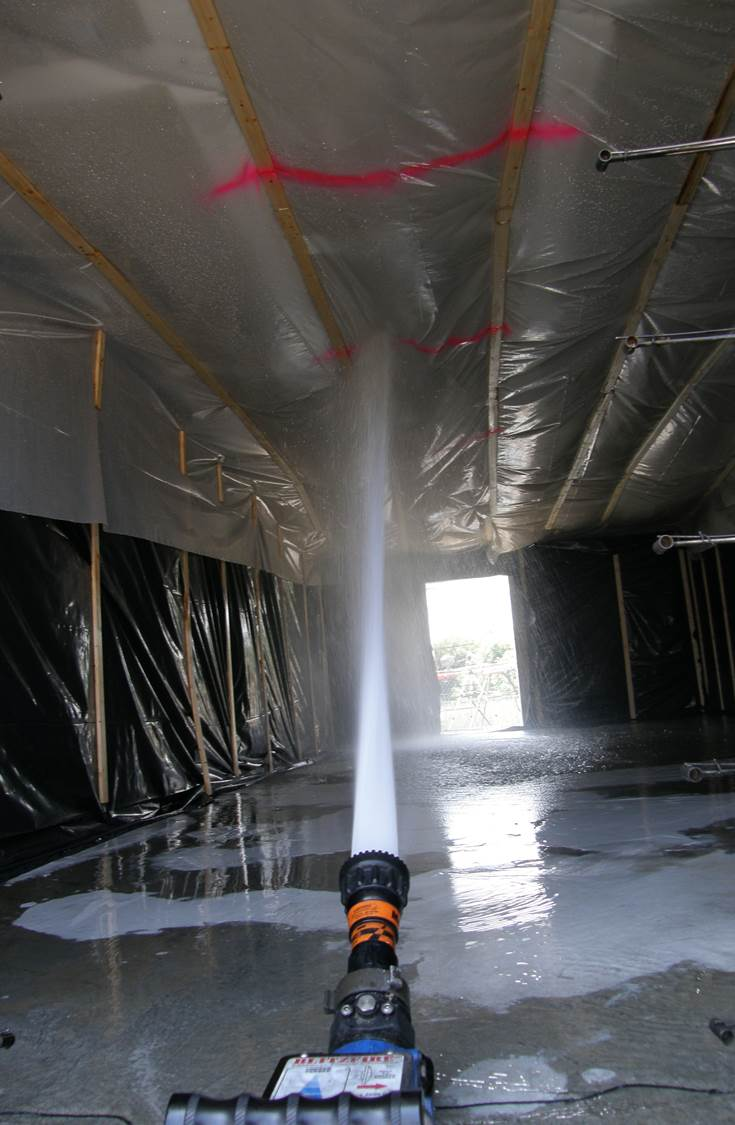
\includegraphics[width=2in]{../Pictures/SS_far}
\end{center} 
\endminipage \hfill
\minipage{2.15in}
\begin{center}
	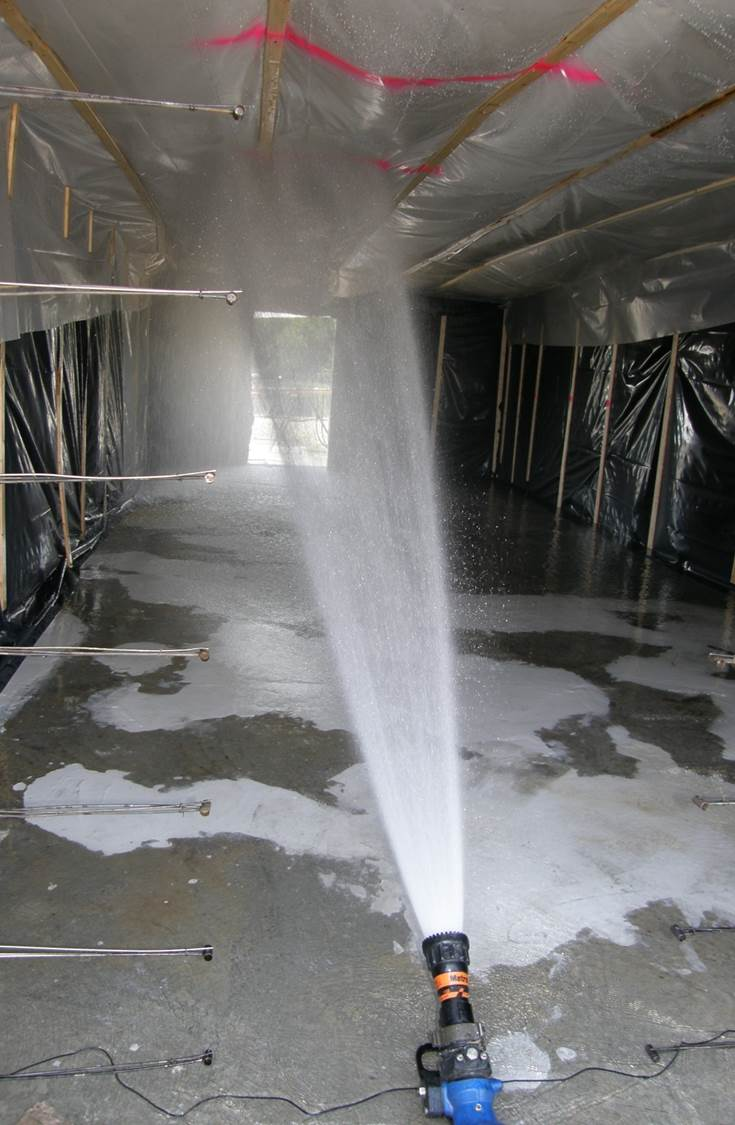
\includegraphics[width=2in]{../Pictures/NF_far}
\end{center}
\endminipage \hfill
\minipage{2.15in}
\begin{center}
	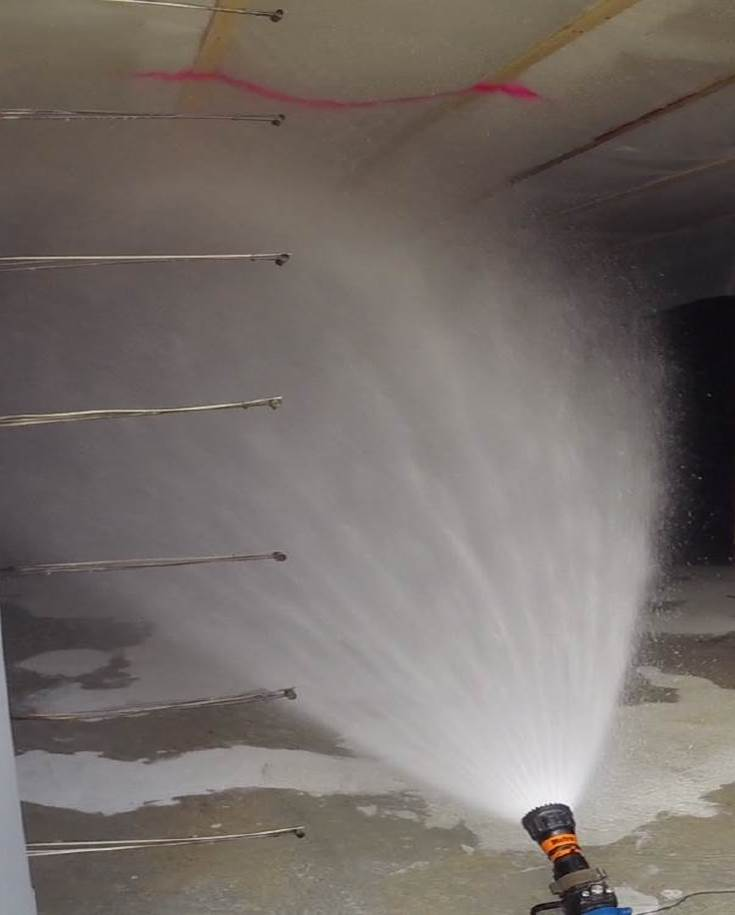
\includegraphics[width=2in]{../Pictures/WF_far}
\end{center}
\endminipage \hfill
\caption[Straight Stream, Narrow Fog Stream, and Wide Fog Stream during Tests 16 and 17]{Straight stream (left column), narrow fog stream (middle column), and wide fog stream (right column) aimed at "near" target (top row) and "far" target (bottom row) during Tests 16 and 17}
\label{fig:test_16_17_pic}
\end{figure}

\clearpage

\subsubsection{Handline Experiments}
\label{sec:Water_Flow_Handline_Procedure}
A total of five sets of experiments were conducted using a 1.75" handline with a combination nozzle to flow water. Three of the tests (Tests 31, 32, and 34) occurred in the East Structure and two of the tests (Tests 18 and 19) occurred in the West Structure. 

Tests 31 and 32 followed an identical procedure that involved flowing water from the north side double doors of the East Structure using a combination nozzle attached to a 1.75" handline. The structure's layout during both tests was identical to the layout used in Tests 29 and 30 (Fig.~\ref{fig:test_29-32_setup}). Each test began by flowing water with the nozzle aimed at the ceiling of Room C in a fixed position, as pictured in Fig.~\ref{fig:test_31_32_pic}. After 30 seconds had elapsed, the nozzle was rotated in the clockwise direction for 30 seconds and then returned to the fixed position for 30 seconds. Next, the nozzle was rotated in the counterclockwise direction for 30 seconds and then returned to the fixed position for 30 seconds. While the nozzle was in the fixed position, the south side door was opened and the application patterns were repeated. After the patterns were applied with the south side door opened, the door was closed, and the process was repeated with the handline aimed at Door BC. The entire procedure was then repeated an additional time. A straight stream pattern was used during Test 31 and a narrow fog stream pattern was used during Test 32.

\begin{figure}[!ht]
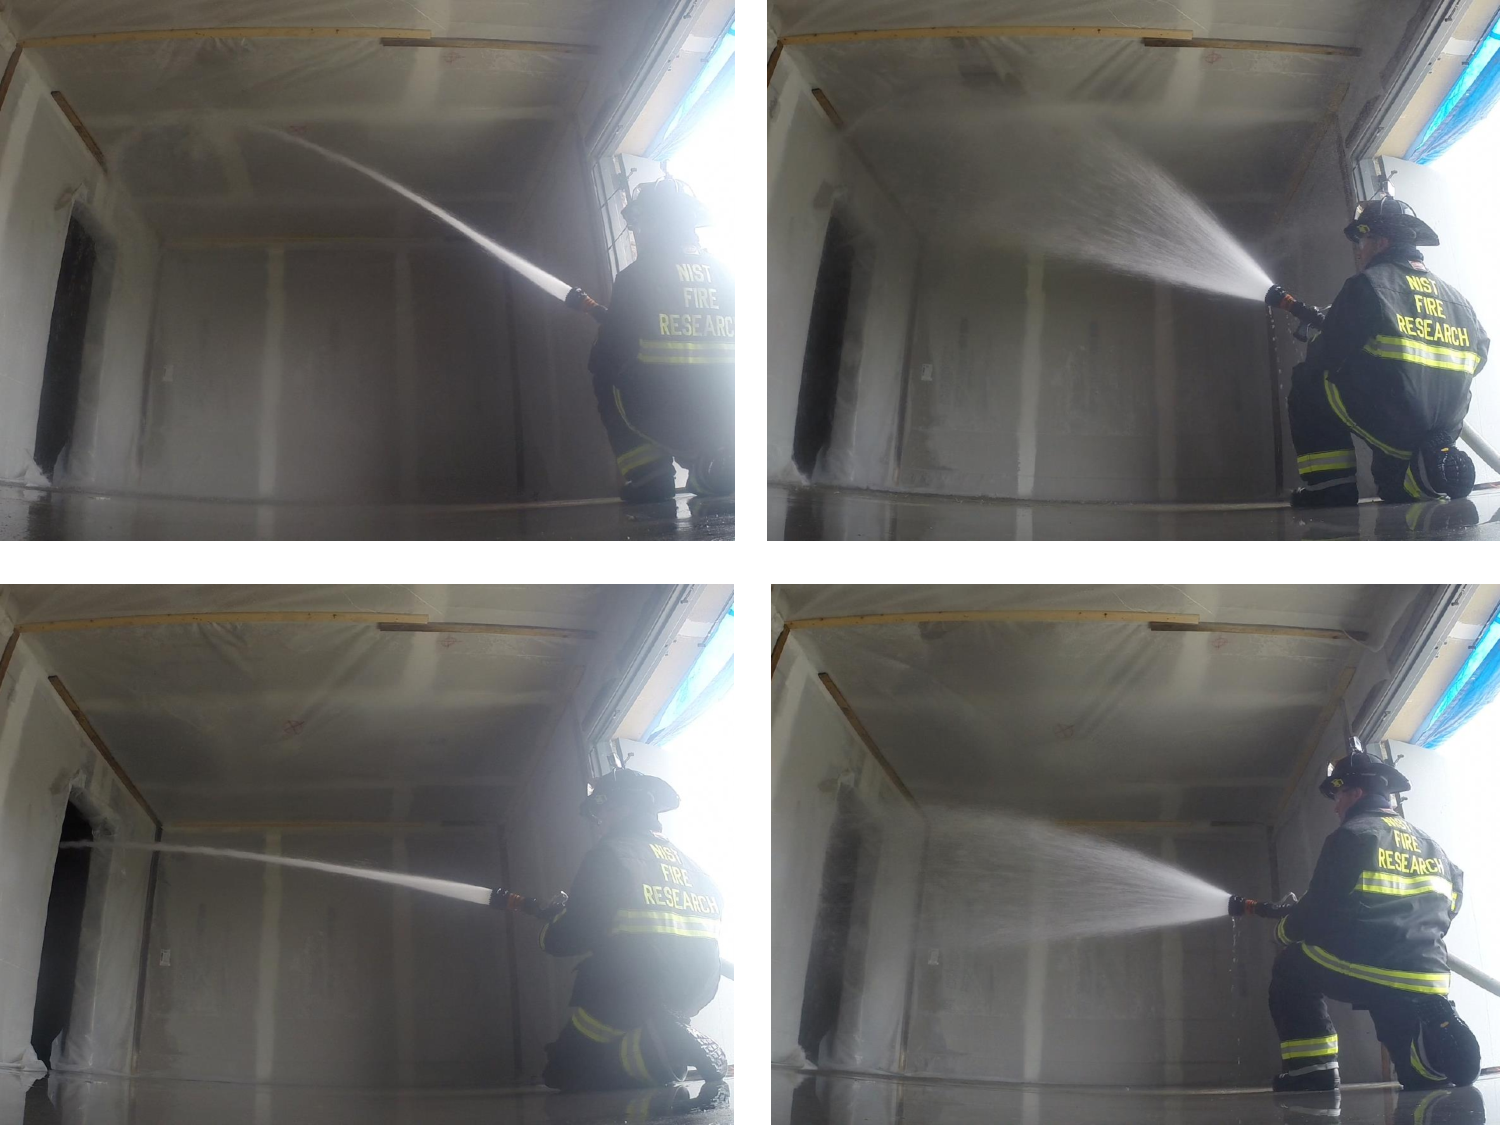
\includegraphics[width=6in]{../Pictures/East_handline_C_BC.pdf}
\caption[Straight Stream and Narrow Fog Stream during Tests 31 and 32]{Straight stream (left column) and narrow fog stream (right column) aimed at ceiling of Room C (top row) and Door BC (bottom row) during Tests 31 and 32}
\label{fig:test_31_32_pic}
\end{figure}
\clearpage

Test 34 varied from Tests 31 and 32 in multiple ways. During Test 34, the handline was located inside Room C. The structure's layout during Test 34 was identical to the layout used in Test 33 (Fig.~\ref{fig:test_33_34_setup}). The test began by flowing water in a straight stream at the ceiling in Room B for 30 seconds in a fixed position, as pictured in Fig.~\ref{fig:test_34_pic}. Next, the nozzle was rotated in the clockwise direction for 30 seconds. Then, the handline was aimed at Door AB, and water was applied for 30 seconds in a fixed position and for 30 seconds in a clockwise pattern. This process were repeated for narrow fog and wide fog streams. Then, the entire procedure was repeated for the three types of streams, except a counter-clockwise pattern was applied.

\begin{figure}[!ht]
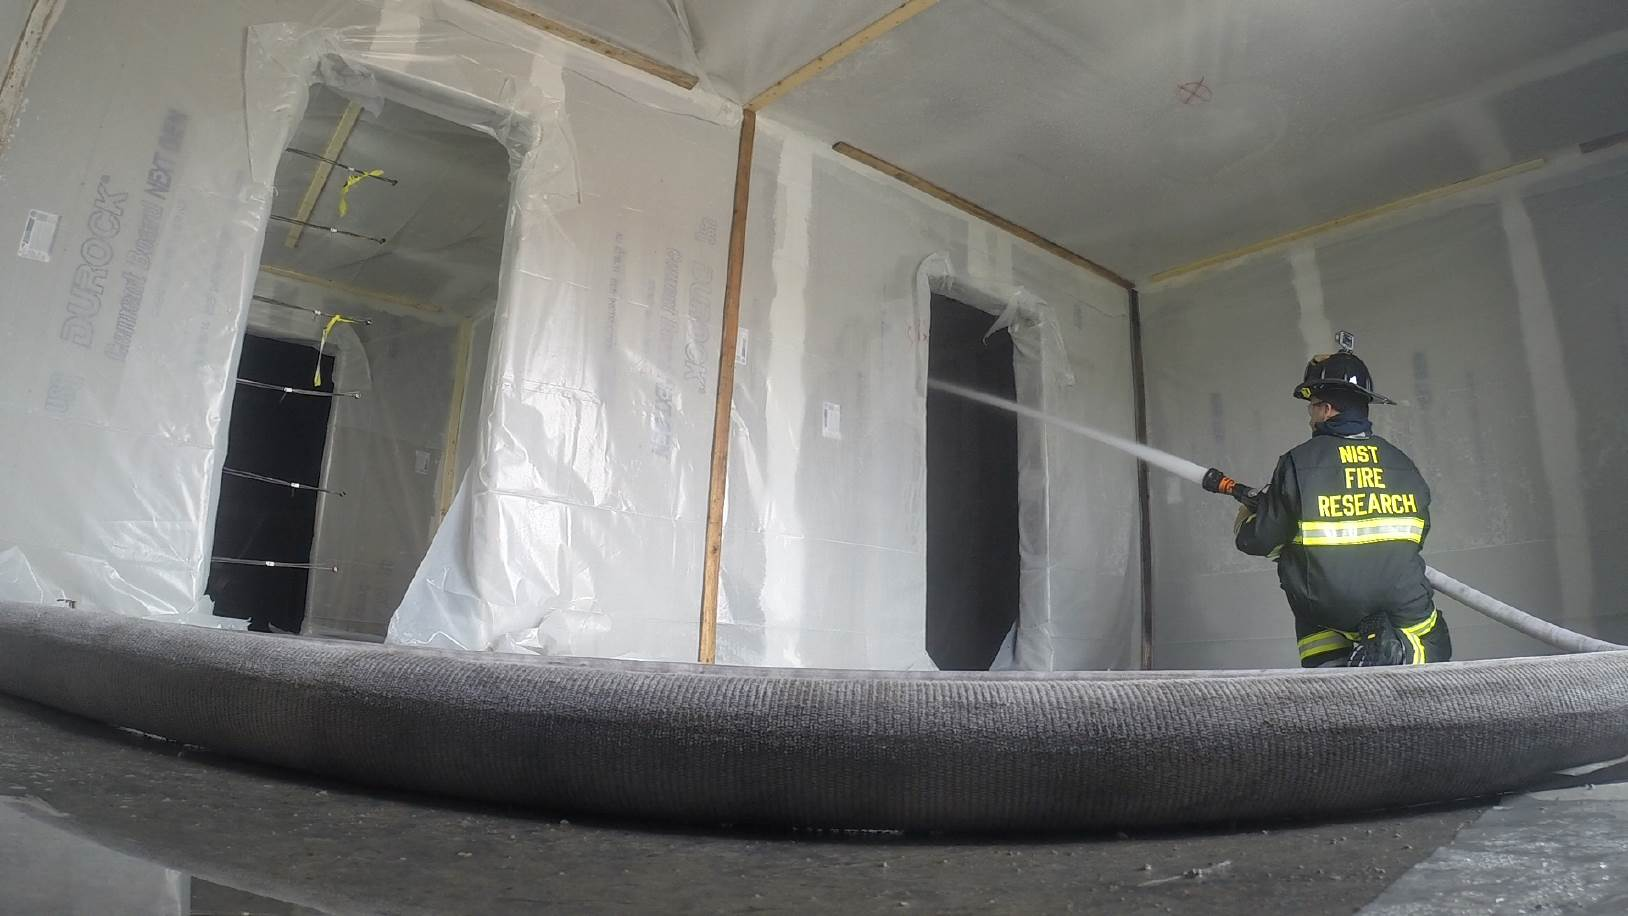
\includegraphics[trim=23cm 6.5cm 4cm 6cm, clip=true, width=3.75in]{../Pictures/SS_Room_B_Test_34}
\\~\\
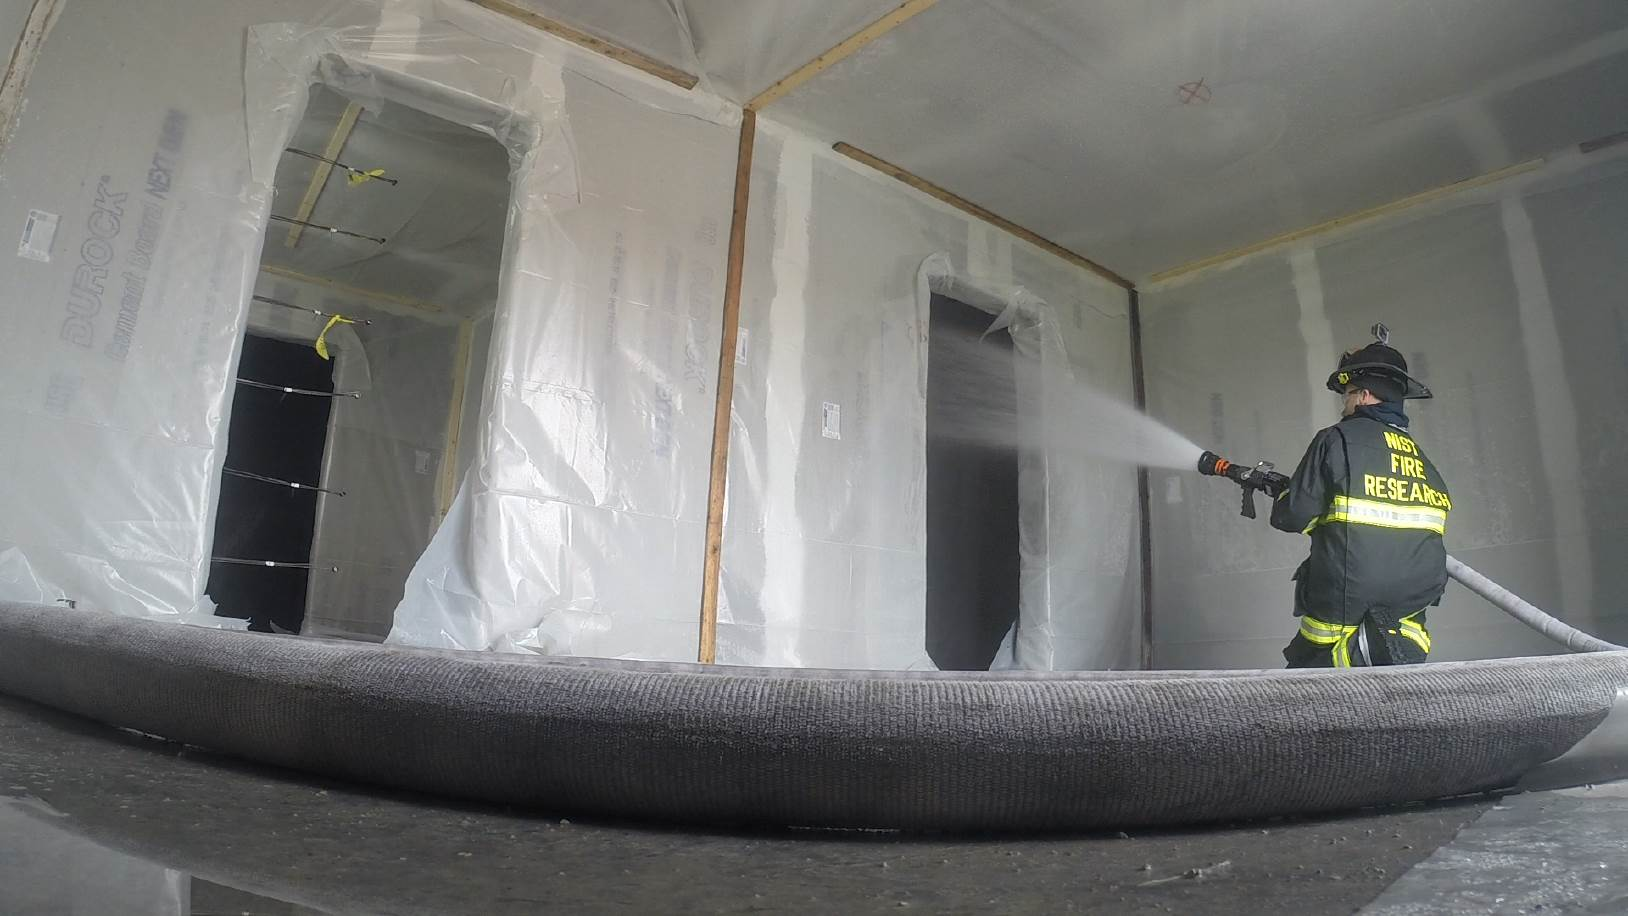
\includegraphics[trim=23cm 6.5cm 4cm 6cm, clip=true, width=3.75in]{../Pictures/NF_Room_B_Test_34}
\\~\\
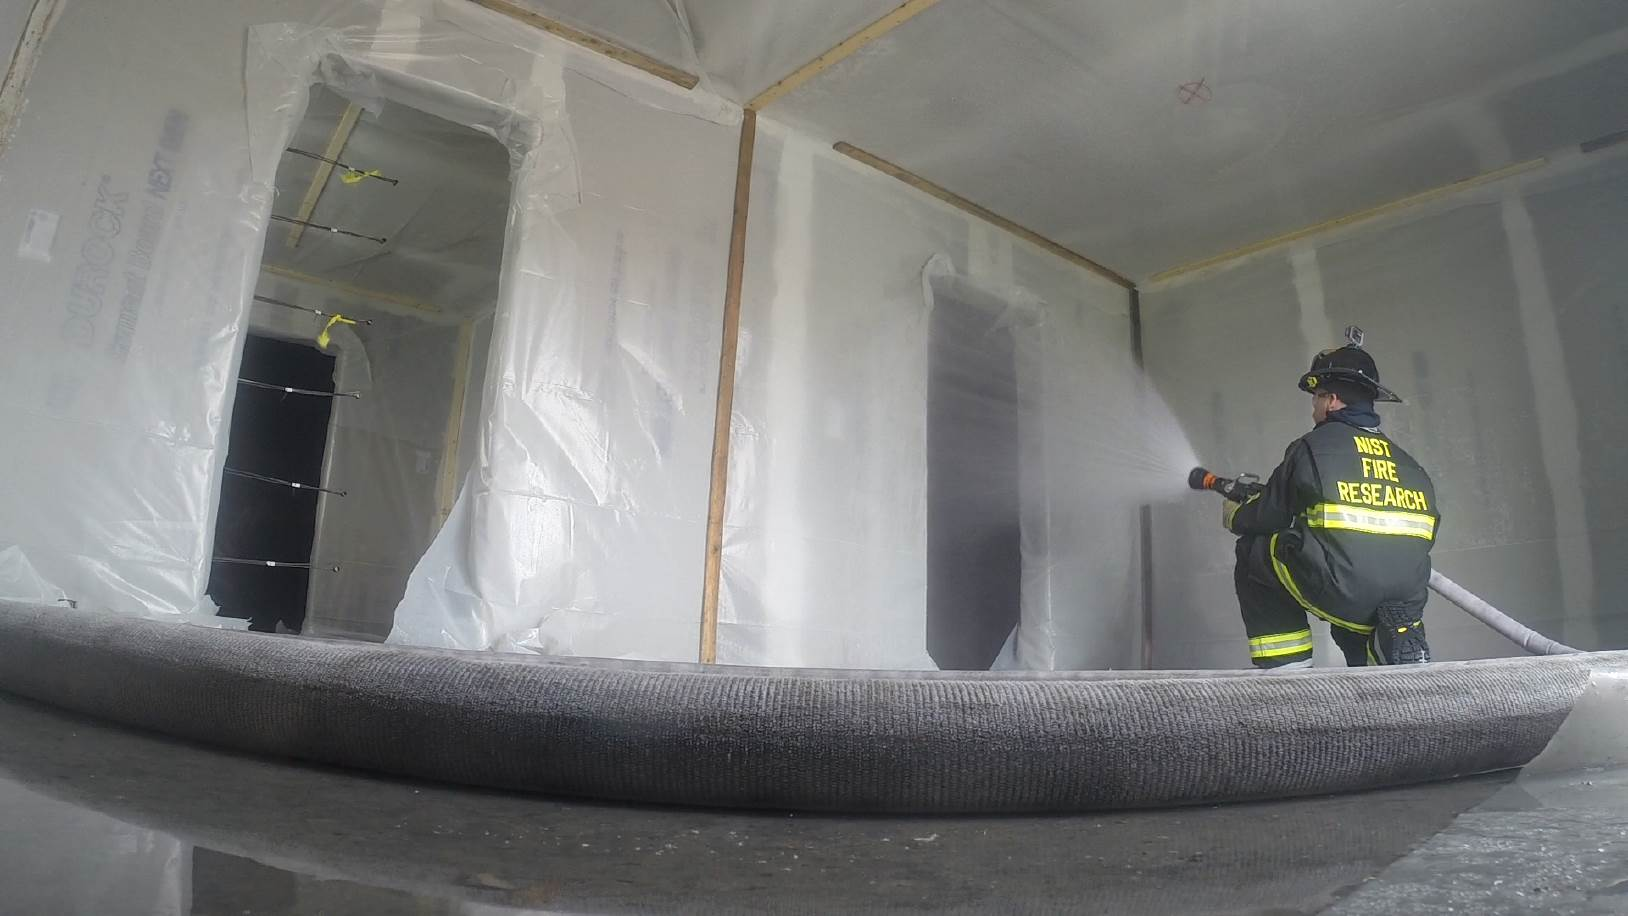
\includegraphics[trim=23cm 6.5cm 4cm 6cm, clip=true, width=3.75in]{../Pictures/WF_Room_B_Test_34}
\caption[Straight Stream, Narrow Fog Stream, and Wide Fog Stream during Test 34]{Straight stream (top), narrow fog stream (middle), and wide fog stream (bottom) aimed at ceiling of Room B during Test 34}
\label{fig:test_34_pic}
\end{figure}
\FloatBarrier

%Where was the handline aimed?%
Tests 18 and 19 followed an identical procedure that involved flowing water from the north side, double doors on the first level of the West Structure using a combination nozzle attached to a 1 \nicefrac{3}{4}" handline. The difference between the two tests was that Test 18 contained the same flow path configuration as Test 16 (Fig.~\ref{fig:flow_path_1}), while Test 19 contained the same flow path configuration as Test 17 (Fig.~\ref{fig:flow_path_2}). Each test began by flowing water in a straight stream pattern and fixed position. After 60 seconds of water flow, the stairwell door was opened. One minute later, the north side, west double door on the second floor was opened, and water continued to flow for 60 seconds. Then, water flow stopped, the two doors were closed, and the procedure was repeated three additional times for sweeping, clockwise, and counterclockwise application patterns. This entire procedure was repeated for narrow fog and wide fog streams.

\begin{figure}[!ht]
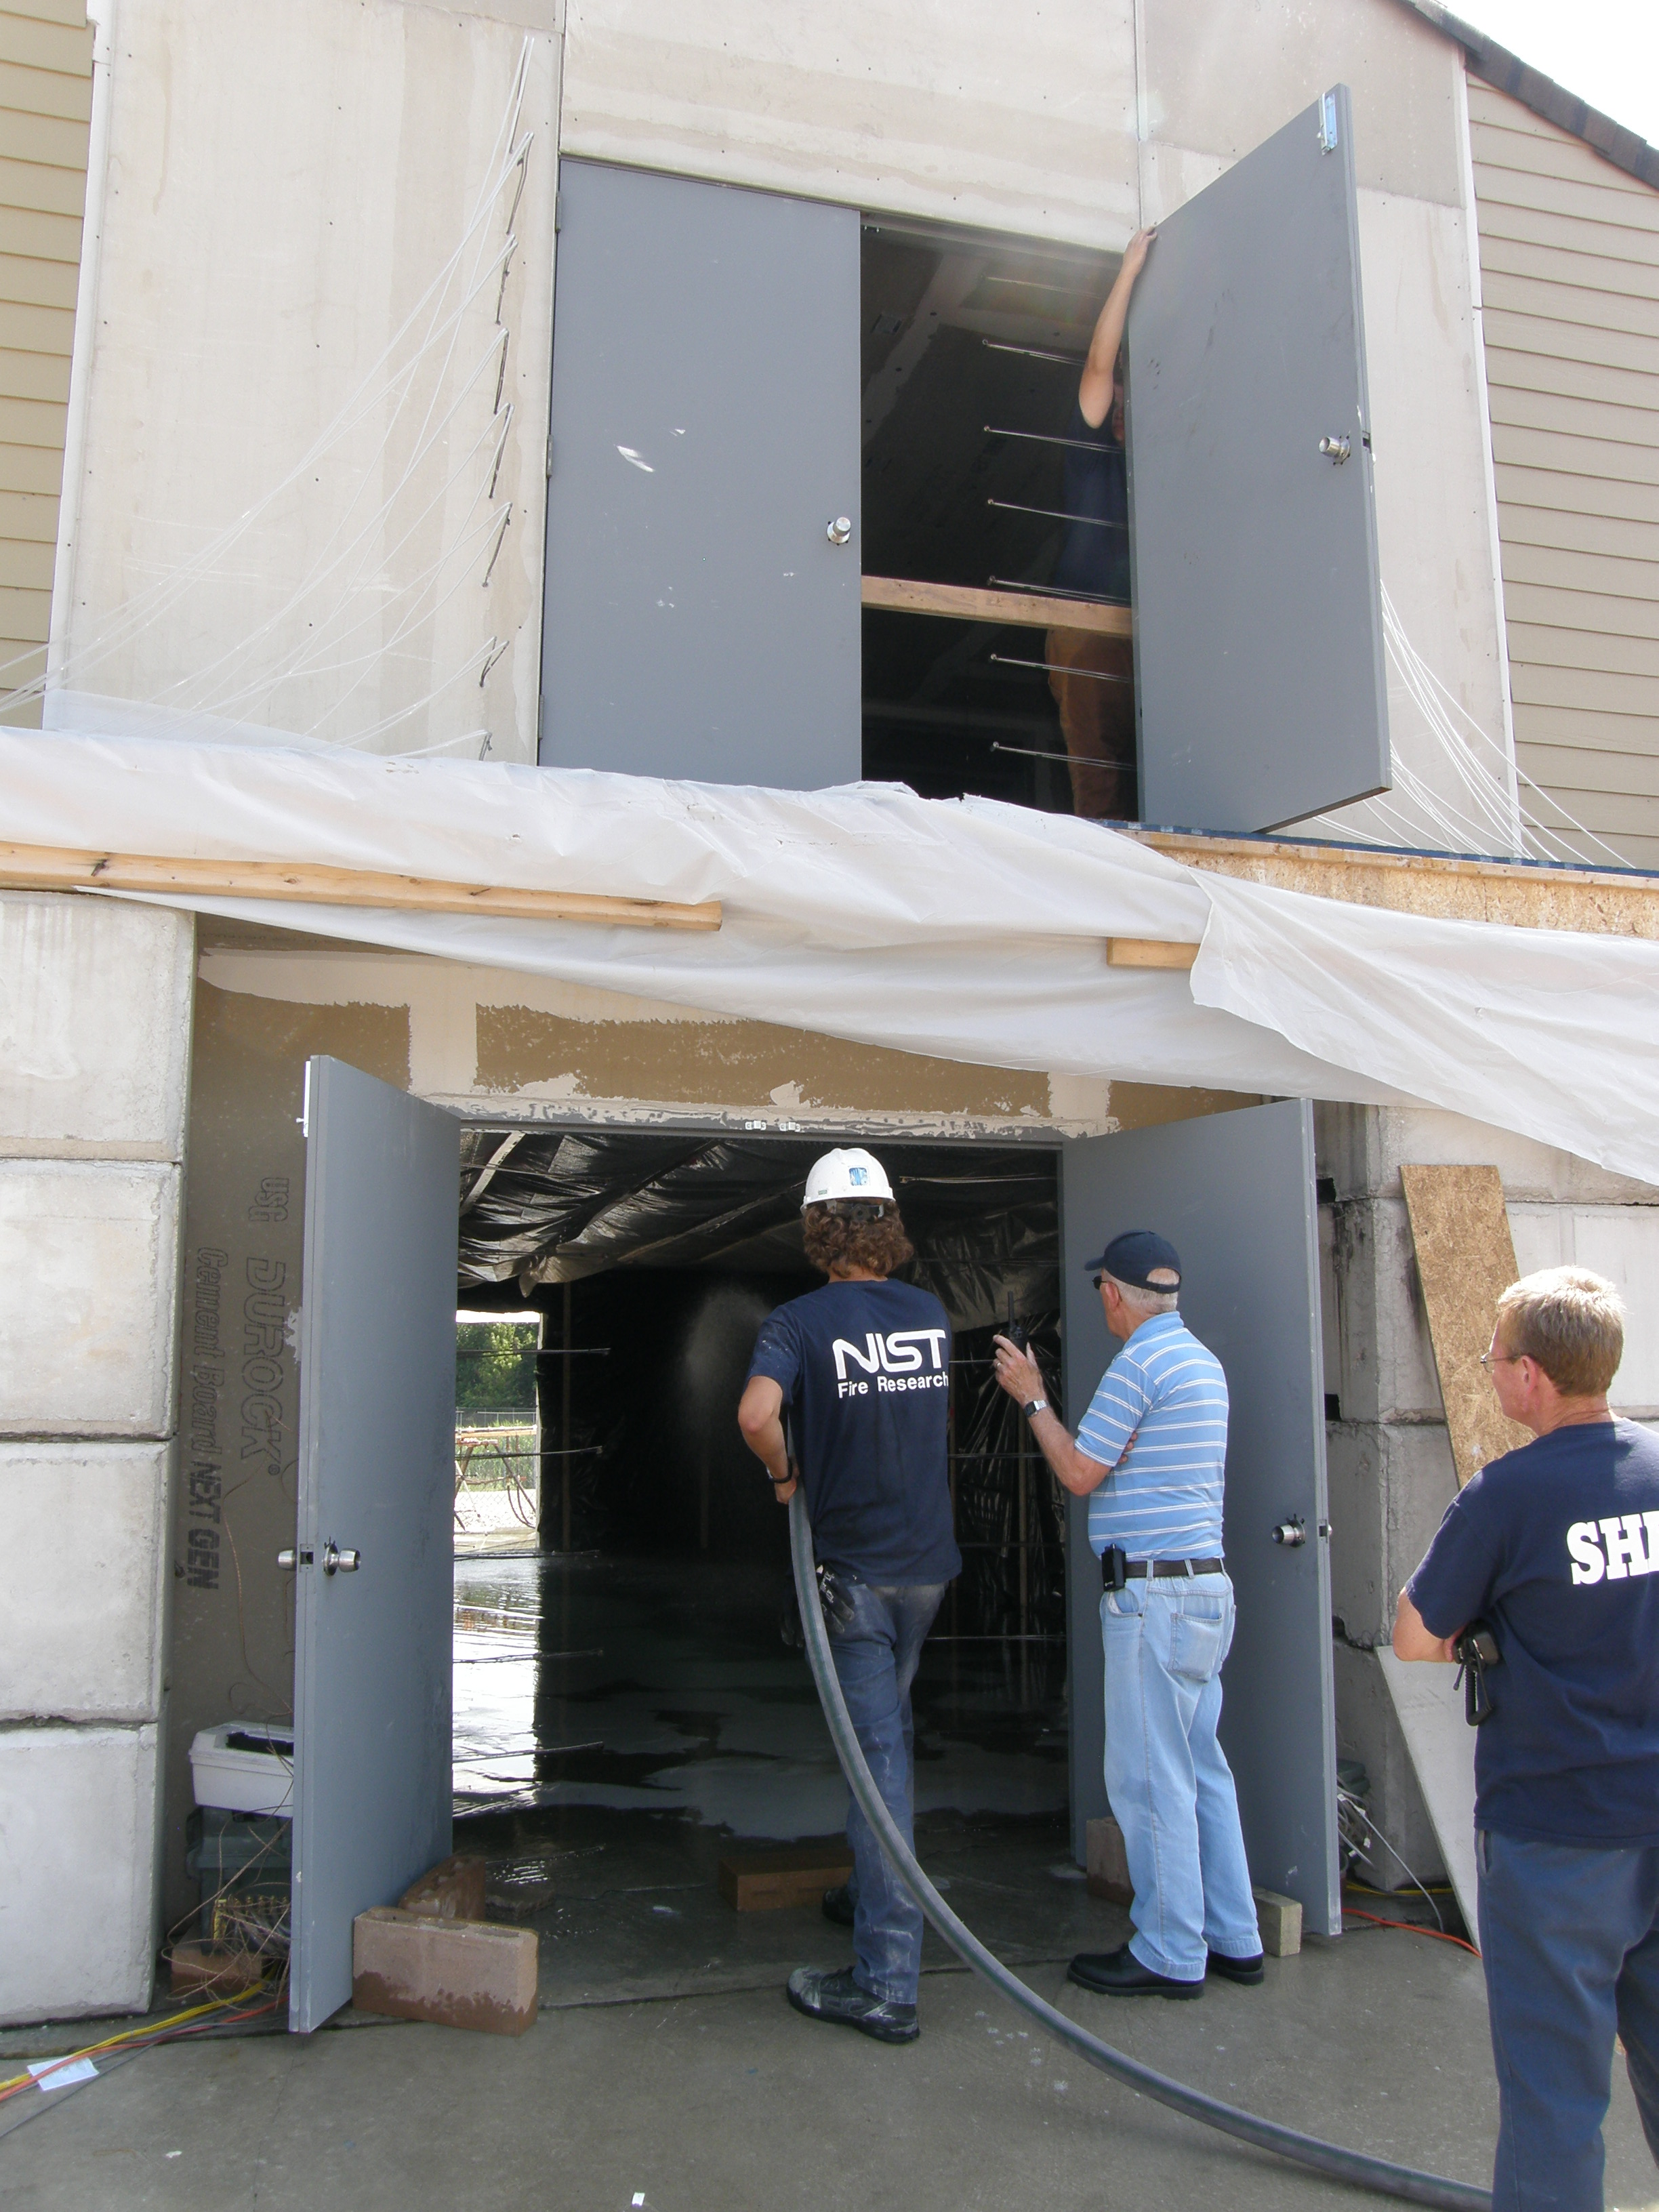
\includegraphics[width=4.25in]{../Pictures/Test_18}
\caption[North Side of West Structure during Test 18]{North side of West Structure during Test 18. A straight stream pattern is being applied, and the flow path is fully established with the stairway door and the north side, west double door both opened.}
\label{fig:test_18_pic}
\end{figure}
\clearpage

\chapter{Results}
\label{chap:Results}

\section{Cold Flow Test Results}
\label{sec:Cold_Flow_Test_Results}

\section{Water Flow Test Results}
\label{sec:Water_Flow_Test_Results}

\subsection{Monitor Nozzle Experiments}

Fig.~\ref{fig:Test_16_BDP_A10_Avg_All} and Fig.~\ref{fig:Test_16_BDP_A13_Avg_All} contain plots of the average velocity measured by the bi-directional probes in the stairwell doorway (A10) and \nth{2} level, north side, west double doorway (A13), respectively, for Test 16. A similar set of plots was generated using data from Test 17 and can be found in Appendix~\ref{sec:additional_figures}.

Notice, the only instances in which significant air movement (average velocity greater than 0.5 m/s) occurs through either doorway is when the flow path is fully established, or when both the stairwell door and the \nth{2} level, north side, west double door are opened. Tables~\ref{table:Tests_16_17_BDP_A10_Avgs} and~\ref{table:Tests_16_17_BDP_A13_Avgs} contain the average air velocity measured by the bi-directional probes at A10 and A13, respectively, when the flow path was completely established for each hose stream pattern and application location for Tests 16 and 17.

\begin{figure}[!ht]
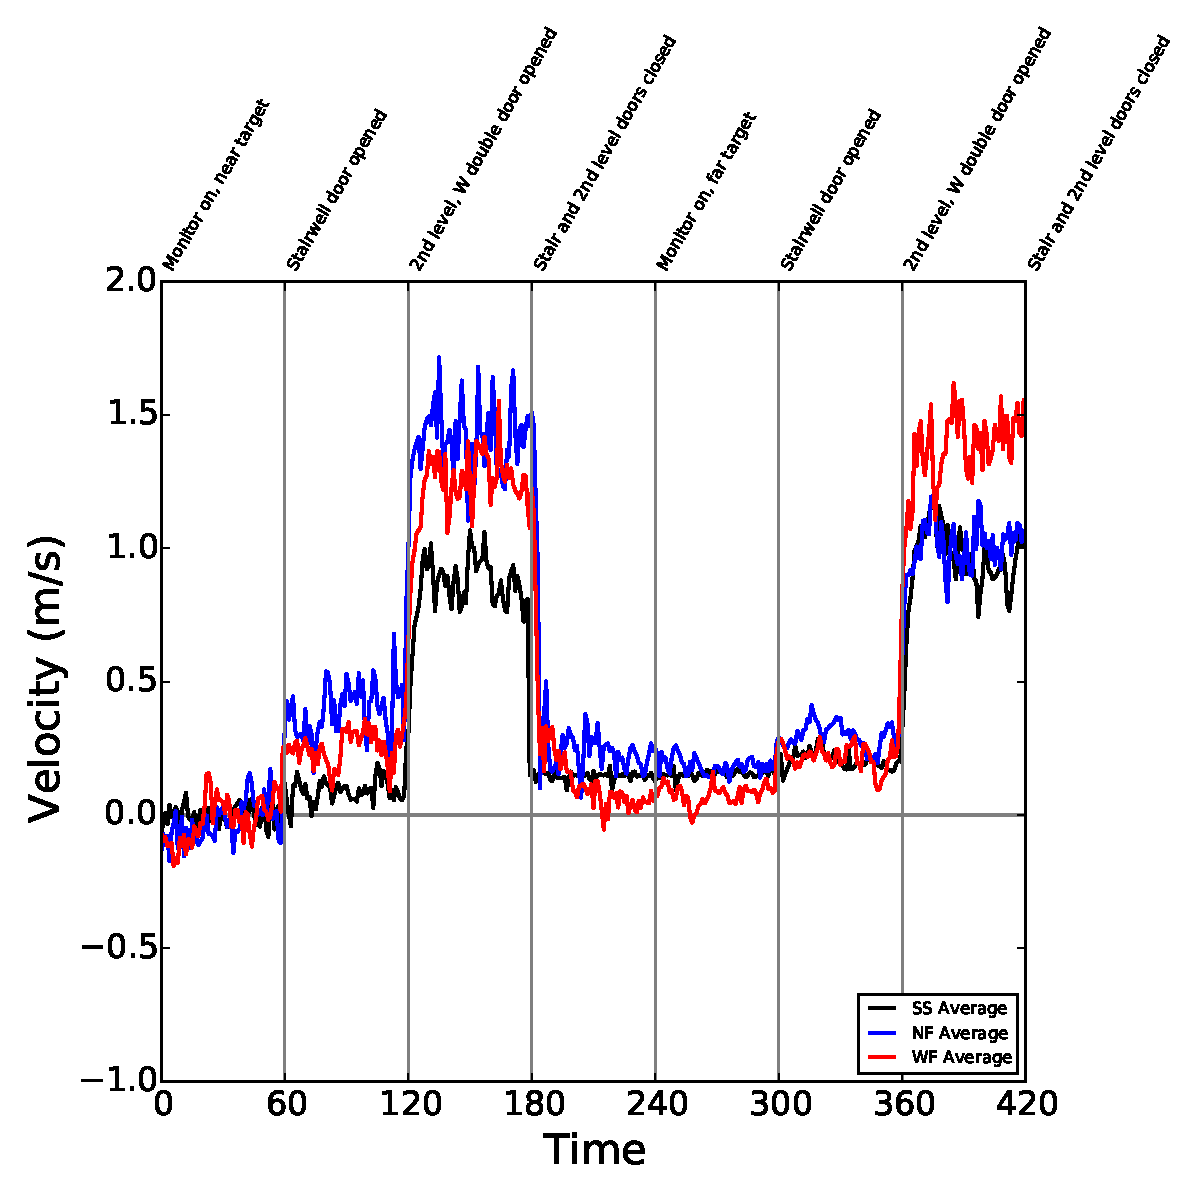
\includegraphics[width=6in]{../../../Figures/Hose_Test_Figures/Test_16_West_063014_custom_BDP_A10_Avg}
\caption{Average Velocity through Stairwell Door, Test 16, All Streams}
\label{fig:Test_16_BDP_A10_Avg_All}
\end{figure}

\begin{figure}[!ht]
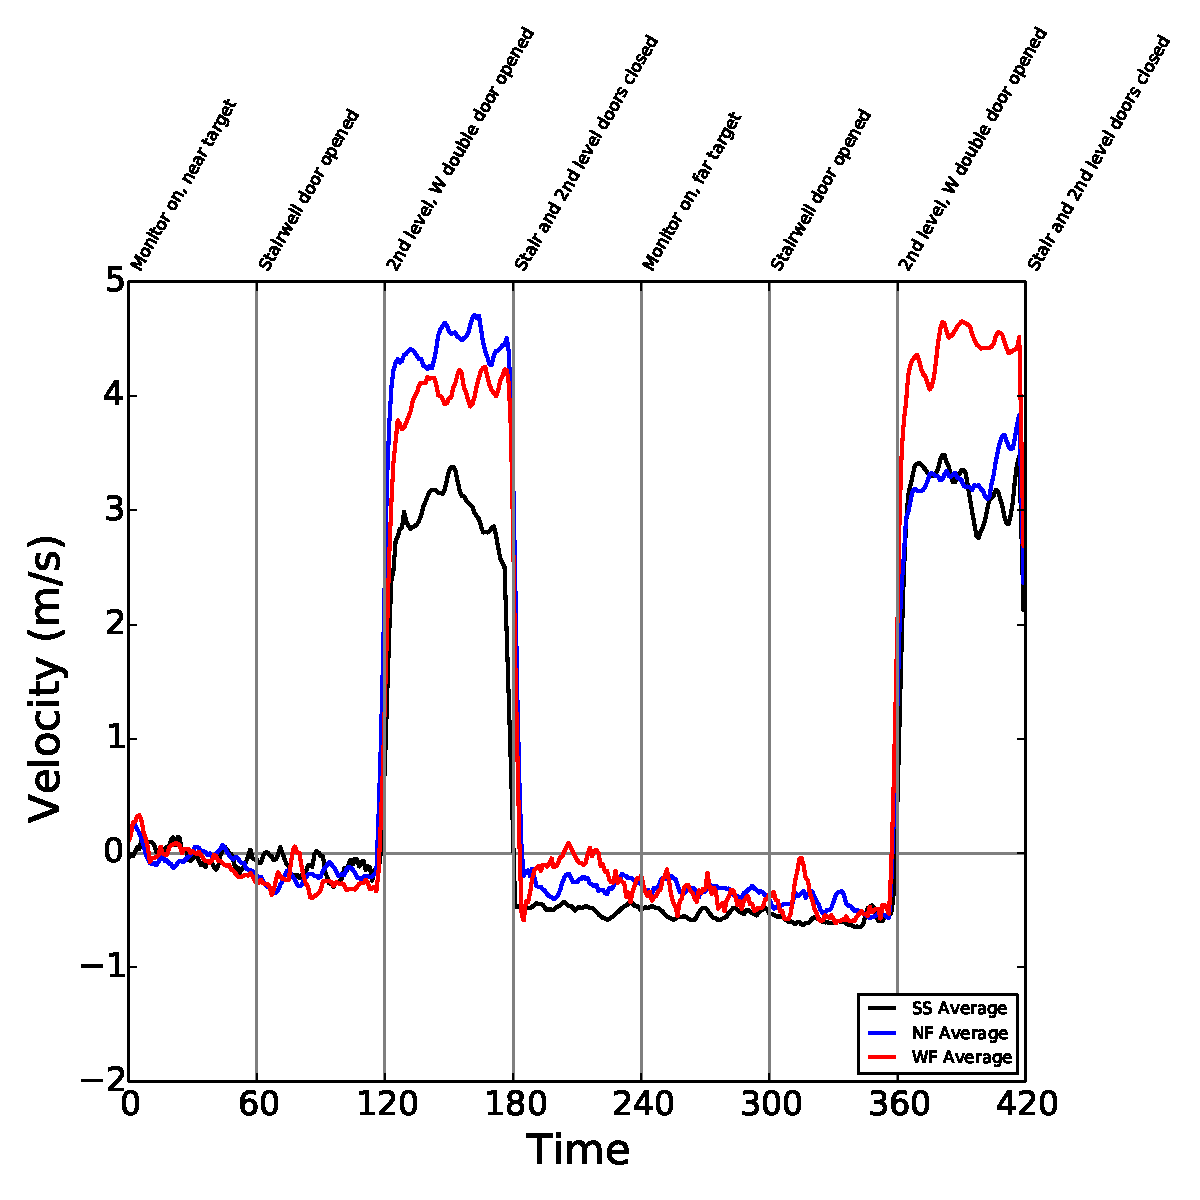
\includegraphics[width=6in]{../../../Figures/Hose_Test_Figures/Test_16_West_063014_custom_BDP_A13_Avg}
\caption{Average Velocity through \nth{2} Level, North Side, West Double Door, Test 16, All Streams}
\label{fig:Test_16_BDP_A13_Avg_All}
\end{figure}

\clearpage



%%%%%%%%%%%%%%%%%%% ORIGINAL TABLES %%%%%%%%%%%%%%%%%%%%%%
%\begin{table}[!ht]
%\caption{Average air velocity (m/s) through stairwell door for all hose stream and application location combinations for Tests 16 and 17}
%\begin{tabular}{|l|c|c|c|c|}
%\cline{2-5}
%\multicolumn{1}{c|}{} & \multicolumn{2}{c|}{Test 16} & \multicolumn{2}{c|}{Test 17} \\ \hline
%\textbf{Stream} & \textbf{Near} & \textbf{Far} & \textbf{Near} & \textbf{Far} \\ \hline
%\textit{Straight} & 
%%%%%Test 16%%%% 
%0.8 $\pm 0.2$ & 0.9 $\pm 0.2$ & 
%%%%%Test 17%%%% 
%0.7 $\pm 0.1$ & 0.7 $\pm 0.2$ \\ \hline
%\textit{Narrow Fog} & 
%%%%%Test 16%%%% 
%1.4 $\pm 0.1$ & 1.0 $\pm 0.1$ & 
%%%%%Test 17%%%% 
%0.8 $\pm 0.2$ & 0.8 $\pm 0.1 $ \\ \hline
%\textit{Wide Fog} 	& 
%%%%%Test 16%%%% 
%1.2 $\pm 0.1$ & 1.4 $\pm 0.1$ & 
%%%%%Test 17%%%% 
%0.9 $\pm 0.2$ & 0.7 $\pm 0.2$ \\ \hline
%\end{tabular}
%\label{table:Tests_16_17_BDP_A10_Avgs}
%\end{table}

%code for higher resolution in tabulated values
%\textit{Straight} & 0.84 & 0.94 & 0.73 & 0.69 \\ \hline
%\textit{Narrow Fog} & 1.41 & 1.00 & 0.75 & 0.75 \\ \hline
%\textit{Wide Fog} & 1.23 & 1.37 & 0.88 & 0.71 \\ \hline

%\begin{table}[!ht]
%\caption{Average air velocity (m/s) through \nth{2} level double door for all hose stream and application location combinations for Tests 16 and 17}
%\begin{tabular}{|l|c|c|c|c|}
%\cline{2-5}
%\multicolumn{1}{c|}{} & \multicolumn{2}{c|}{Test 16} & \multicolumn{2}{c|}{Test 17} \\ \hline
%\textbf{Stream} & \textbf{Near} & \textbf{Far} & \textbf{Near} & \textbf{Far} \\ \hline
%\textit{Straight} 	& 
%%%%%Test 16%%%% 
%2.8 $\pm 0.6$ & 3.1 $\pm 0.5$ & 
%%%%%Test 17%%%% 
%2.7 $\pm 0.4$ & 2.3 $\pm 0.8$ \\ \hline
%\textit{Narrow Fog} & 
%%%%%Test 16%%%% 
%4.4 $\pm 0.3$ & 3.3 $\pm 0.4$ & 
%%%%%Test 17%%%% 
%2.6 $\pm 0.6$ & 2.7 $\pm 0.6$ \\ \hline
%\textit{Wide Fog} 	& 
%%%%%Test 16%%%% 
%3.9 $\pm 0.5$ & 4.4 $\pm 0.3$ & 
%%%%%Test 17%%%% 
%3.1 $\pm 0.7$ & 2.8 $\pm 0.7$ \\ \hline
%\end{tabular}
%\label{table:Tests_16_17_BDP_A13_Avgs}
%\end{table}

%code for higher resolution in tabulated values
%\textit{Straight} 	& 2.82 & 3.10 & 2.66 & 2.33 \\ \hline
%\textit{Narrow Fog} & 4.39 & 3.26 & 2.58 & 2.68 \\ \hline
%\textit{Wide Fog} 	& 3.92 & 4.37 & 3.14 & 2.76 \\ \hline


\begin{table}[!ht]
\caption{Average air velocity (m/s) through stairwell door for all hose stream and application location combinations when the flow path was fully established during Tests 16 and 17}
\begin{tabular}{lcccc}
\toprule
 & \multicolumn{2}{c}{\underline{Test 16}} & \multicolumn{2}{c}{\underline{Test 17}}
\\
\textbf{Stream} & \textbf{Near} & \textbf{Far} & \textbf{Near} & \textbf{Far} \\
\midrule
\textit{Straight} & 
%%%%Test 16%%%% 
0.8 $\pm 0.2$ & 0.9 $\pm 0.2$ & 
%%%%Test 17%%%% 
0.7 $\pm 0.1$ & 0.7 $\pm 0.2$
\\	\multicolumn{5}{c}{}	\\
\textit{Narrow Fog} & 
%%%%Test 16%%%% 
1.4 $\pm 0.1$ & 1.0 $\pm 0.1$ & 
%%%%Test 17%%%% 
0.8 $\pm 0.2$ & 0.8 $\pm 0.1 $          
\\	\multicolumn{5}{c}{}	\\
\textit{Wide Fog} 	& 
%%%%Test 16%%%% 
1.2 $\pm 0.1$ & 1.4 $\pm 0.1$ & 
%%%%Test 17%%%% 
0.9 $\pm 0.2$ & 0.7 $\pm 0.2$
\\
\bottomrule
\end{tabular}
\label{table:Tests_16_17_BDP_A10_Avgs}
\end{table}

\begin{table}[!ht]
\caption{Average air velocity (m/s) through \nth{2} level double door for all hose stream and application location combinations when the flow path was fully established during Tests 16 and 17}
\begin{tabular}{lcccc}
\toprule
 & \multicolumn{2}{c}{\underline{Test 16}} & \multicolumn{2}{c}{\underline{Test 17}}
\\
\textbf{Stream} & \textbf{Near} & \textbf{Far} & \textbf{Near} & \textbf{Far} \\
\midrule
\textit{Straight} & 
%%%%Test 16%%%% 
2.8 $\pm 0.6$ & 3.1 $\pm 0.5$ & 
%%%%Test 17%%%% 
2.7 $\pm 0.4$ & 2.3 $\pm 0.8$
\\	\multicolumn{5}{c}{}	\\
\textit{Narrow Fog} & 
%%%%Test 16%%%% 
4.4 $\pm 0.3$ & 3.3 $\pm 0.4$ & 
%%%%Test 17%%%% 
2.6 $\pm 0.6$ & 2.7 $\pm 0.6$
\\	\multicolumn{5}{c}{}	\\
\textit{Wide Fog} 	& 
%%%%Test 16%%%% 
3.9 $\pm 0.5$ & 4.4 $\pm 0.3$ & 
%%%%Test 17%%%% 
3.1 $\pm 0.7$ & 2.8 $\pm 0.7$ 
\\ 
\bottomrule
\end{tabular}
\label{table:Tests_16_17_BDP_A13_Avgs}
\end{table}


\subsection{Handline Experiments}

Figures \ref{fig:Test_18_BDP_A10_Avg_All}-\ref{fig:Test_19_BDP_A13_Avg_All} contain plots of the average velocity through the stairwell door and \nth{2} level, north side, west double door, measured by the bi-directional probes in each doorway for the four application patterns and three hose stream patterns for Tests 18 and 19. 

\begin{figure}[!ht]
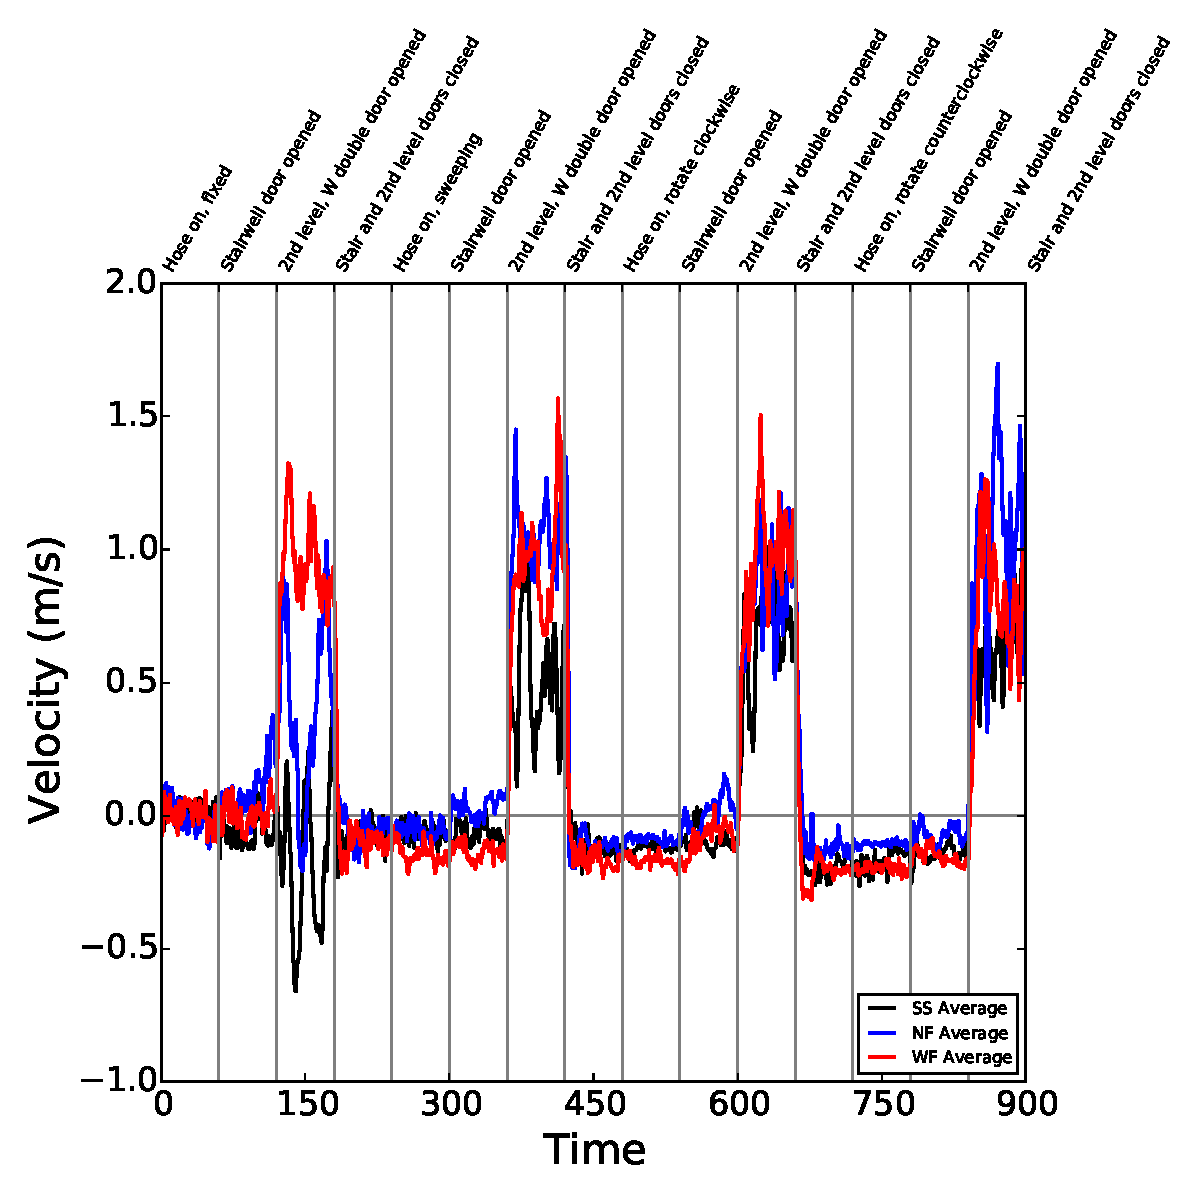
\includegraphics[width=6in]{../../../Figures/Hose_Test_Figures/Test_18_West_063014_BDP_A10_Avg}
\caption{Average Velocity through Stairwell Door, Test 18, All Streams}
\label{fig:Test_18_BDP_A10_Avg_All}
\end{figure}

\begin{figure}[!ht]
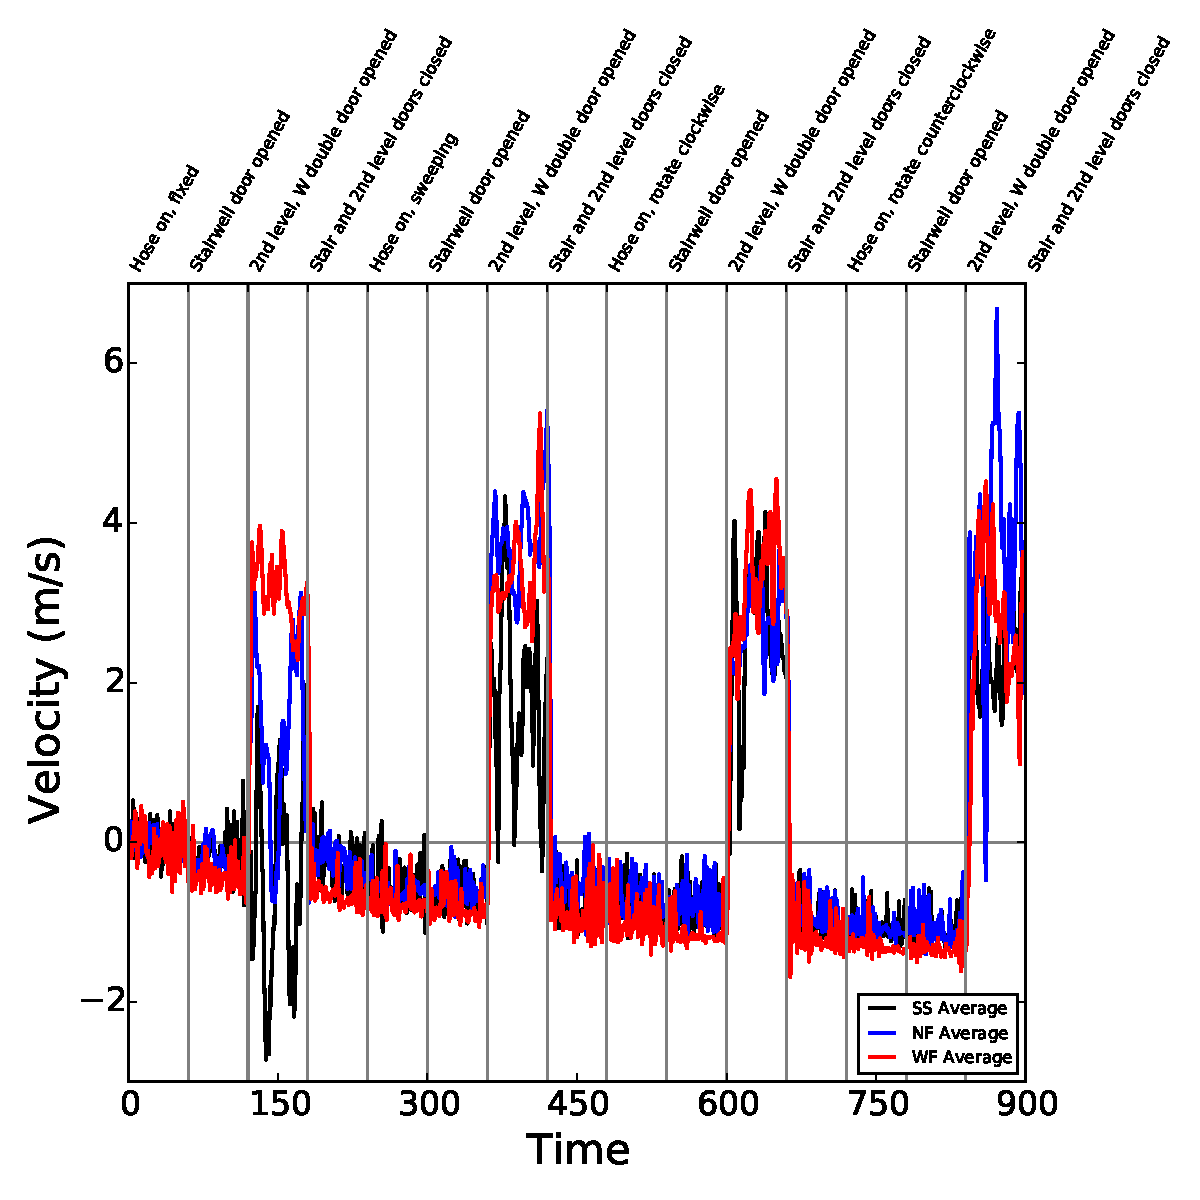
\includegraphics[width=6in]{../../../Figures/Hose_Test_Figures/Test_18_West_063014_BDP_A13_Avg}
\caption{Average Velocity through \nth{2} Level, North Side, West Double Door, Test 18, All Streams}
\label{fig:Test_18_BDP_A13_Avg_All}
\end{figure}

\clearpage

\begin{figure}[!ht]
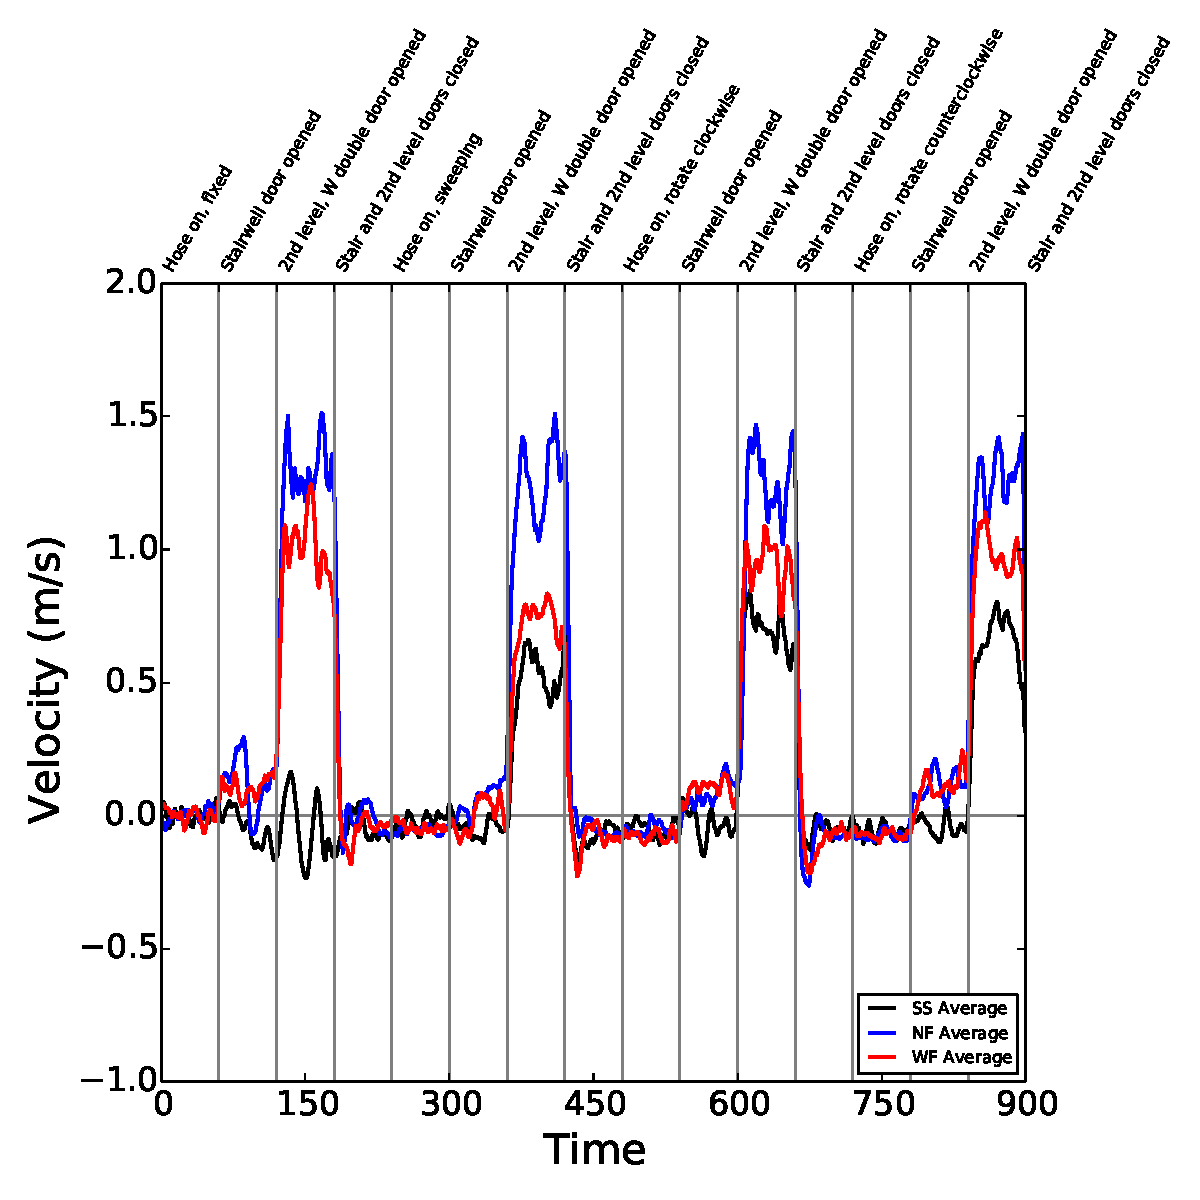
\includegraphics[width=6in]{../../../Figures/Hose_Test_Figures/Test_19_West_063014_BDP_A10_Avg}
\caption{Average Velocity through Stairwell Door, Test 19, All Streams}
\label{fig:Test_19_BDP_A10_Avg_All}
\end{figure}

\begin{figure}[!ht]
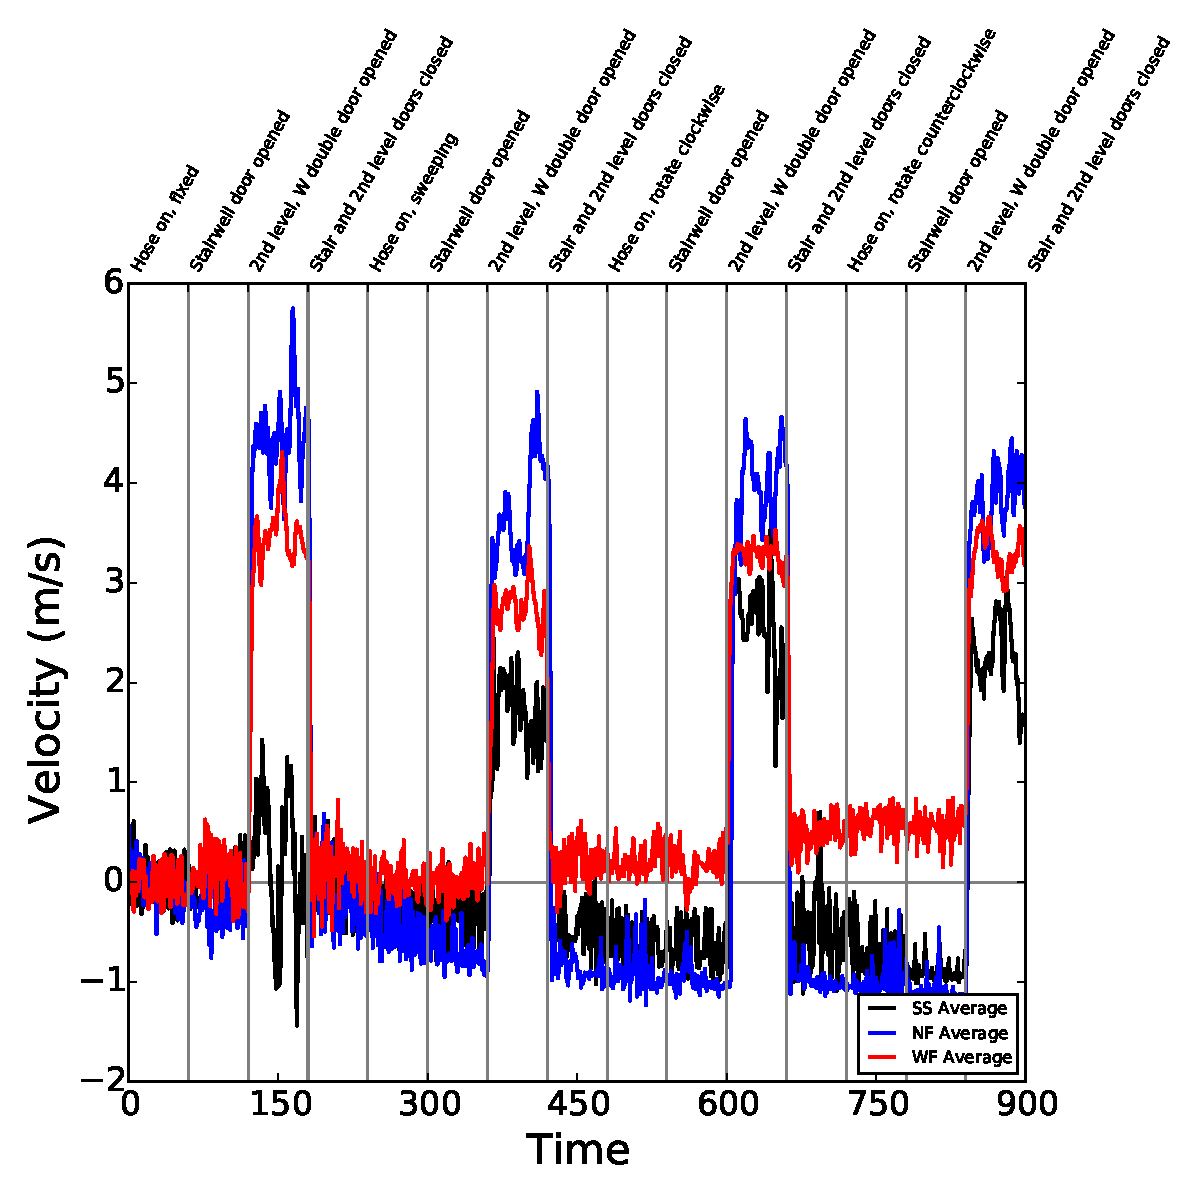
\includegraphics[width=6in]{../../../Figures/Hose_Test_Figures/Test_19_West_063014_BDP_A13_Avg}
\caption{Average Velocity through \nth{2} Level, North Side, West Double Door, Test 19, All Streams}
\label{fig:Test_19_BDP_A13_Avg_All}
\end{figure}

\clearpage

Significant air flow through the stairwell and \nth{2} level double door only occurred when the flow path was complete, or when both doors were in the open position. Tables~\ref{table:Tests_18_19_BDP_A10_Avgs} and \ref{table:Tests_18_19_BDP_A13_Avgs} contain the average air velocity measured by the eight BDPs at the stairwell door and \nth{2} level, double door, respectively, during the time the flow path was complete for each application pattern and hose stream combination used during Tests 18 and 19.

%%%%%%%%%%%%%%%%%%%%%%% ORIGINAL TABLES %%%%%%%%%%%%%%%%%%%%%%%%%%%%%%%%%%%%%
%\begin{table}[!ht]
%\addtolength{\tabcolsep}{-3.25pt}
%\small
%\caption{Average air velocity (m/s) through stairwell door for all hose stream and application pattern combinations for Tests 18 and 19}
%\begin{tabular}{|l|c|c|c|c|c|c|c|c|}
%\cline{2-9}
%\multicolumn{1}{c|}{} & \multicolumn{4}{c|}{Test 18} & \multicolumn{4}{c|}{Test 19} \\ \hline
%\textbf{Stream} & \textbf{Fixed} & \textbf{Sweeping} & \textbf{Clockwise} & \begin{tabular}{@{}c@{}} \textbf{Counter} \\ \textbf{Clockwise} \\ \end{tabular} & \textbf{Fixed} & \textbf{Sweeping} & \textbf{Clockwise} & \begin{tabular}{@{}c@{}} \textbf{Counter} \\ \textbf{Clockwise} \\ \end{tabular} \\ \hline
%%%%%%%%%%%%%%%%%%%%%%%%%%%%%%%%%%%%%%%%%%%%%%%%%%%%%%%%%%%%%%
%\textit{Straight} 	& 
%%%%%Test 18%%%% 
%-0.2 $\pm 0.3$ & 0.5 $\pm 0.2$ & 0.7 $\pm 0.2$ & 0.6 $\pm 0.2$ & 
%%%%%Test 19%%%% 
% 0.0 $\pm 0.1$ & 0.5 $\pm 0.2$ & 0.7 $\pm 0.2$ & 0.6 $\pm 0.2$ \\ \hline
%\textit{Narrow Fog} & 
%%%%%Test 18%%%% 
% 0.4 $\pm 0.3$ & 1.0 $\pm 0.2$ & 0.8 $\pm 0.2$ & 1.0 $\pm 0.4$ & 
%%%%%Test 19%%%% 
% 1.2 $\pm 0.3$ & 1.2 $\pm 0.3$ & 1.1 $\pm 0.4$ & 1.2 $\pm 0.2$ \\ \hline
%\textit{Wide Fog} 	& 
%%%%%Test 18%%%% 
% 0.9 $\pm 0.2$ & 0.9 $\pm 0.3$ & 0.9 $\pm 0.3$ & 0.8 $\pm 0.3$ & 
%%%%%Test 19%%%% 
% 1.0 $\pm 0.2$ & 0.7 $\pm 0.2$ & 0.9 $\pm 0.2$ & 0.9 $\pm 0.2$ \\ \hline
%\end{tabular}
%\label{table:Tests_18_19_BDP_A10_Avgs}
%\end{table}
%
%%code to increase resolution of tabulated values
%%\textit{Straight} 	& -0.17 & 0.48 & 0.65 & 0.63 & -0.05 & 0.47 & 0.67 & 0.62 \\ \hline
%%\textit{Narrow Fog} & 0.41 & 1.02 & 0.79 & 0.99 & 1.23 & 1.18 & 1.14 & 1.22 \\ \hline
%%\textit{Wide Fog} 	& 0.93 & 0.90 & 0.91 & 0.75 & 0.96 & 0.67 & 0.89 & 0.93 \\ \hline
%
%\begin{table}[!ht]
%\addtolength{\tabcolsep}{-3.25pt}
%\small
%\caption{Average air velocity (m/s) through \nth{2} level double door for all hose stream and application pattern combinations for Tests 18 and 19}
%\begin{tabular}{|l|c|c|c|c|c|c|c|c|}
%\cline{2-9}
%\multicolumn{1}{c|}{} & \multicolumn{4}{c|}{Test 18} & \multicolumn{4}{c|}{Test 19} \\ \hline
%\textbf{Stream} & \textbf{Fixed} & \textbf{Sweeping} & \textbf{Clockwise} & \begin{tabular}{@{}c@{}} \textbf{Counter} \\ \textbf{Clockwise} \\ \end{tabular} & \textbf{Fixed} & \textbf{Sweeping} & \textbf{Clockwise} & \begin{tabular}{@{}c@{}} \textbf{Counter} \\ \textbf{Clockwise} \\ \end{tabular} \\ \hline
%%%%%%%%%%%%%%%%%%%%%%%%%%%%%%%%%%%%%%%%%%%%%%%%%%%%%%%%%%%%%%
%\textit{Straight}  &
%%%%%Test 18%%%% 
%-0.4 $\pm 1.3$ & 1.8 $\pm 1.1$ & 2.5 $\pm 1.1$ & 2.4 $\pm 0.8$ &
%%%%%Test 19%%%%					
% 0.2 $\pm 0.7$ & 1.6 $\pm 0.5$ & 2.5 $\pm 0.7$ & 2.1 $\pm 0.7$ \\ \hline
%\textit{Narrow Fog} & 
%%%%%Test 18%%%%
% 1.3 $\pm 1.1$ & 3.6 $\pm 0.9$ & 2.6 $\pm 0.8$ & 3.5 $\pm 1.6$ & 
%%%%%Test 19%%%%
% 4.3 $\pm 1.0$ & 3.5 $\pm 1.0$ & 3.5 $\pm 1.5$ & 3.7 $\pm 0.9$ \\ \hline
%\textit{Wide Fog} 	& 
%%%%%Test 18%%%%
%3.0 $\pm 0.7$ & 3.2 $\pm 1.0$ & 3.1 $\pm 1.1$ & 2.6 $\pm 1.3$ & 
%%%%%Test 19%%%%
%3.3 $\pm 0.7$ & 2.6 $\pm 0.6$ & 3.1 $\pm 0.6$ & 3.2 $\pm 0.5$ \\ \hline
%\end{tabular}
%\label{table:Tests_18_19_BDP_A13_Avgs}
%\end{table}
%
%%code to increase resolution of tabulated values
%%\textit{Straight} 	& -0.43 & 1.75 & 2.46 & 2.40 & 0.20 & 1.60 & 2.47 & 2.10 \\ \hline
%%\textit{Narrow Fog} & 1.34 & 3.61 & 2.55 & 3.48 & 4.26 & 3.48 & 3.49 & 3.66 \\ \hline
%%\textit{Wide Fog} 	& 3.02 & 3.22 & 3.06 & 2.57 & 3.31 & 2.60 & 3.13 & 3.19 \\ \hline


\begin{table}[!ht]
%\addtolength{\tabcolsep}{-3.25pt}
%\small
\caption{Average air velocity (m/s) through stairwell door for all hose stream and application pattern combinations for Tests 18 and 19}
\begin{tabular}{lcccc}
\toprule
 & \multicolumn{4}{c}{\underline{Test 18}}
\\
\textbf{Stream} & \textbf{Fixed} & \textbf{Sweeping} & \textbf{Clockwise} & \begin{tabular}{@{}c@{}} \textbf{Counter} \\ \textbf{Clockwise} \\ \end{tabular}
\\
\midrule 
%%%%%%%%%%%%%%%%%%%%%%%%%%%%%%%%%%%%%%%%%%%%%%%%%%%%%%%%%%%%%
\textit{Straight} 	& 
%%%%Test 18%%%% 
-0.2 $\pm 0.3$ & 0.5 $\pm 0.2$ & 0.7 $\pm 0.2$ & 0.6 $\pm 0.2$ 
\\	\multicolumn{5}{c}{}	\\
\textit{Narrow Fog} & 
%%%%Test 18%%%% 
 0.4 $\pm 0.3$ & 1.0 $\pm 0.2$ & 0.8 $\pm 0.2$ & 1.0 $\pm 0.4$ 
\\	\multicolumn{5}{c}{}	\\
\textit{Wide Fog} 	& 
%%%%Test 18%%%% 
 0.9 $\pm 0.2$ & 0.9 $\pm 0.3$ & 0.9 $\pm 0.3$ & 0.8 $\pm 0.3$ 
\\
\midrule
& \multicolumn{4}{c}{\underline{Test 19}} 
\\
\textbf{Stream} & \textbf{Fixed} & \textbf{Sweeping} & \textbf{Clockwise} & \begin{tabular}{@{}c@{}} \textbf{Counter} \\ \textbf{Clockwise} \\ \end{tabular}
\\
\midrule
%%%%%%%%%%%%%%%%%%%%%%%%%%%%%%%%%%%%%%%%%%%%%%%%%%%%%%%%%%%%%
\textit{Straight} 	& 
%%%%Test 19%%%% 
 0.0 $\pm 0.1$ & 0.5 $\pm 0.2$ & 0.7 $\pm 0.2$ & 0.6 $\pm 0.2$ 
\\	\multicolumn{5}{c}{}	\\
\textit{Narrow Fog} & 
%%%%Test 19%%%% 
 1.2 $\pm 0.3$ & 1.2 $\pm 0.3$ & 1.1 $\pm 0.4$ & 1.2 $\pm 0.2$
\\	\multicolumn{5}{c}{}	\\
\textit{Wide Fog} 	& 
%%%%Test 19%%%% 
 1.0 $\pm 0.2$ & 0.7 $\pm 0.2$ & 0.9 $\pm 0.2$ & 0.9 $\pm 0.2$
\\
\bottomrule
\end{tabular}
\label{table:Tests_18_19_BDP_A10_Avgs}
\end{table}

\begin{table}[!ht]
%\addtolength{\tabcolsep}{-3.25pt}
%\small
\caption{Average air velocity (m/s) through \nth{2} level double door for all hose stream and application pattern combinations for Tests 18 and 19}
\begin{tabular}{lcccc}
\toprule
 & \multicolumn{4}{c}{\underline{Test 18}}
\\
\textbf{Stream} & \textbf{Fixed} & \textbf{Sweeping} & \textbf{Clockwise} & \begin{tabular}{@{}c@{}} \textbf{Counter} \\ \textbf{Clockwise} \\ \end{tabular}
\\
\midrule 
%%%%%%%%%%%%%%%%%%%%%%%%%%%%%%%%%%%%%%%%%%%%%%%%%%%%%%%%%%%%%
\textit{Straight}  &
%%%%Test 18%%%% 
-0.4 $\pm 1.3$ & 1.8 $\pm 1.1$ & 2.5 $\pm 1.1$ & 2.4 $\pm 0.8$
\\	\multicolumn{5}{c}{}	\\
\textit{Narrow Fog} & 
%%%%Test 18%%%%
 1.3 $\pm 1.1$ & 3.6 $\pm 0.9$ & 2.6 $\pm 0.8$ & 3.5 $\pm 1.6$
 \\	\multicolumn{5}{c}{}	\\ 
\textit{Wide Fog} 	& 
%%%%Test 18%%%%
3.0 $\pm 0.7$ & 3.2 $\pm 1.0$ & 3.1 $\pm 1.1$ & 2.6 $\pm 1.3$
\\
\midrule
 & \multicolumn{4}{c}{\underline{Test 19}}	\\ 
\textbf{Stream} & \textbf{Fixed} & \textbf{Sweeping} & \textbf{Clockwise} & \begin{tabular}{@{}c@{}} \textbf{Counter} \\ \textbf{Clockwise} \\ \end{tabular}
\\
\midrule
\textit{Straight}  &
%%%%Test 19%%%%					
 0.2 $\pm 0.7$ & 1.6 $\pm 0.5$ & 2.5 $\pm 0.7$ & 2.1 $\pm 0.7$ 
 \\	\multicolumn{5}{c}{}	\\
\textit{Narrow Fog} & 
%%%%Test 19%%%%
 4.3 $\pm 1.0$ & 3.5 $\pm 1.0$ & 3.5 $\pm 1.5$ & 3.7 $\pm 0.9$
\\	\multicolumn{5}{c}{}	\\
\textit{Wide Fog} 	& 
%%%%Test 19%%%%
3.3 $\pm 0.7$ & 2.6 $\pm 0.6$ & 3.1 $\pm 0.6$ & 3.2 $\pm 0.5$
\\
\bottomrule
\end{tabular}
\label{table:Tests_18_19_BDP_A13_Avgs}
\end{table}

Notice, there is a significant difference between the average air velocity caused by the fixed straight stream and the velocity caused by the narrow and wide fog streams; the velocities for the narrow and wide fog were always significantly higher than the velocity of the fixed stream. It was only when the hose began to move around that the air velocity through the doorways for the straight stream approached the air velocities associated with the narrow and wide fogs for the corresponding pattern. However, the straight stream hose pattern always resulted in the lowest average air velocity through each doorway for the three different hose streams at each of the four application patterns. 

Another important result shown in Figures \ref{fig:Test_18_BDP_A10_Avg_All} and \ref{fig:Test_19_BDP_A10_Avg_All} and in Tables \ref{table:Tests_18_19_BDP_A10_Avgs} and \ref{table:Tests_18_19_BDP_A13_Avgs} is that there is statistically no significant difference in the amount of air flow through the doorways between rotating the hoseline in the clockwise and counter clockwise directions for the three hose streams tested. 

%\begin{figure}[!ht]
%\includegraphics[width=6in]{../../Figures/Hose_Test_Figures/Test_18_West_063014_BDP_A10_Avg_CW_vs_CCW}
%\caption{Average Velocity of Stairwell Door, Test 18, All Streams, CW vs. CCW}
%\label{fig:Test_18_BDP_A10_Avg_CW_vs_CCW}
%\end{figure}
%
%\begin{figure}[!ht]
%\includegraphics[width=6in]{../../Figures/Hose_Test_Figures/Test_19_West_063014_BDP_A10_Avg_CW_vs_CCW}
%\caption{Average Velocity of Stairwell Door, Test 19, All Streams, CW vs. CCW}
%\label{fig:Test_19_BDP_A10_Avg_CW_vs_CCW}
%\end{figure}
%
%\clearpage
%
%\begin{figure}[!ht]
%\includegraphics[width=6in]{../../Figures/Hose_Test_Figures/Test_18_West_063014_BDP_A13_Avg_CW_vs_CCW}
%\caption{Average Velocity of \nth{2} Level Double Door, Test 18, All Streams, CW vs. CCW}
%\label{fig:Test_18_BDP_A13_Avg_CW_vs_CCW}
%\end{figure}
%
%\clearpage
%
%\begin{figure}[!ht]
%\includegraphics[width=6in]{../../Figures/Hose_Test_Figures/Test_19_West_063014_BDP_A13_Avg_CW_vs_CCW}
%\caption{Average Velocity of \nth{2} Level Double Door, Test 19, All Streams, CW vs. CCW}
%\label{fig:Test_19_BDP_A13_Avg_CW_vs_CCW}
%\end{figure}
%
%\clearpage

\chapter{Conclusions}
\label{chap:Conclusions}

\chapter{Future Work}
\label{chap:Future_Work}

\chapter{Acknowledgments}
\label{chap:Acknowledgments}

\bibliography{../../../../../Bibliography/FDS_general}

\appendix
\chapter{Appendix}
\label{chap:appendix}

\section{Additional Figures}
\label{sec:additional_figures}

\begin{figure}[!ht]
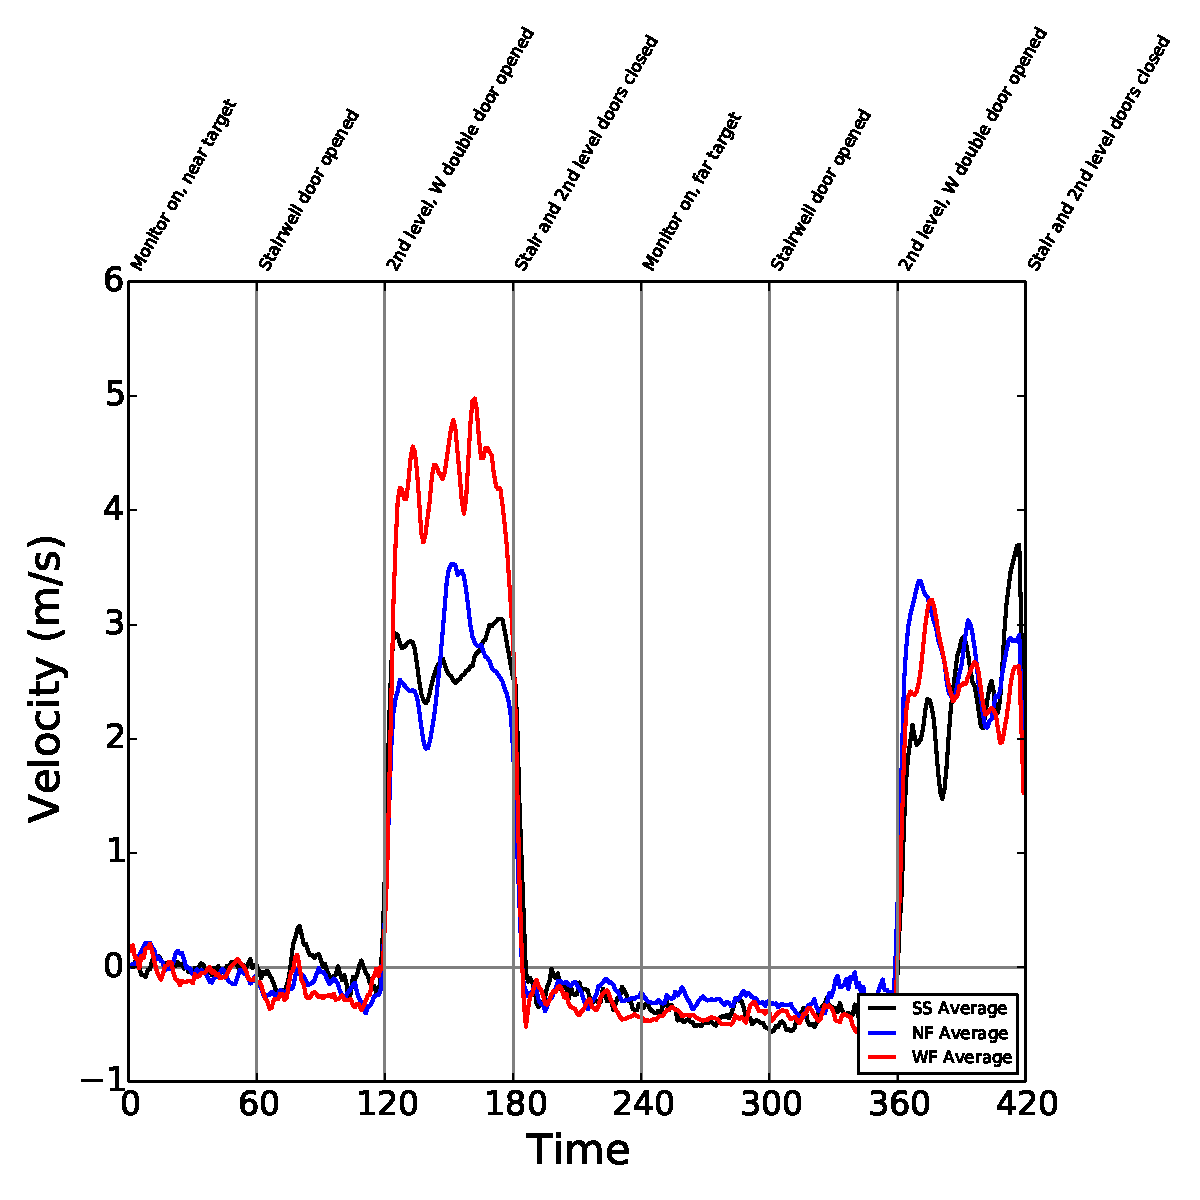
\includegraphics[width=6in]{../../../Figures/Hose_Test_Figures/Test_17_West_063014_BDP_A13_Avg}
\caption{Average Velocity through Stairwell Door, Test 17, All Streams}
\label{fig:Test_17_BDP_A10_Avg_All}
\end{figure}

\begin{figure}[!ht]
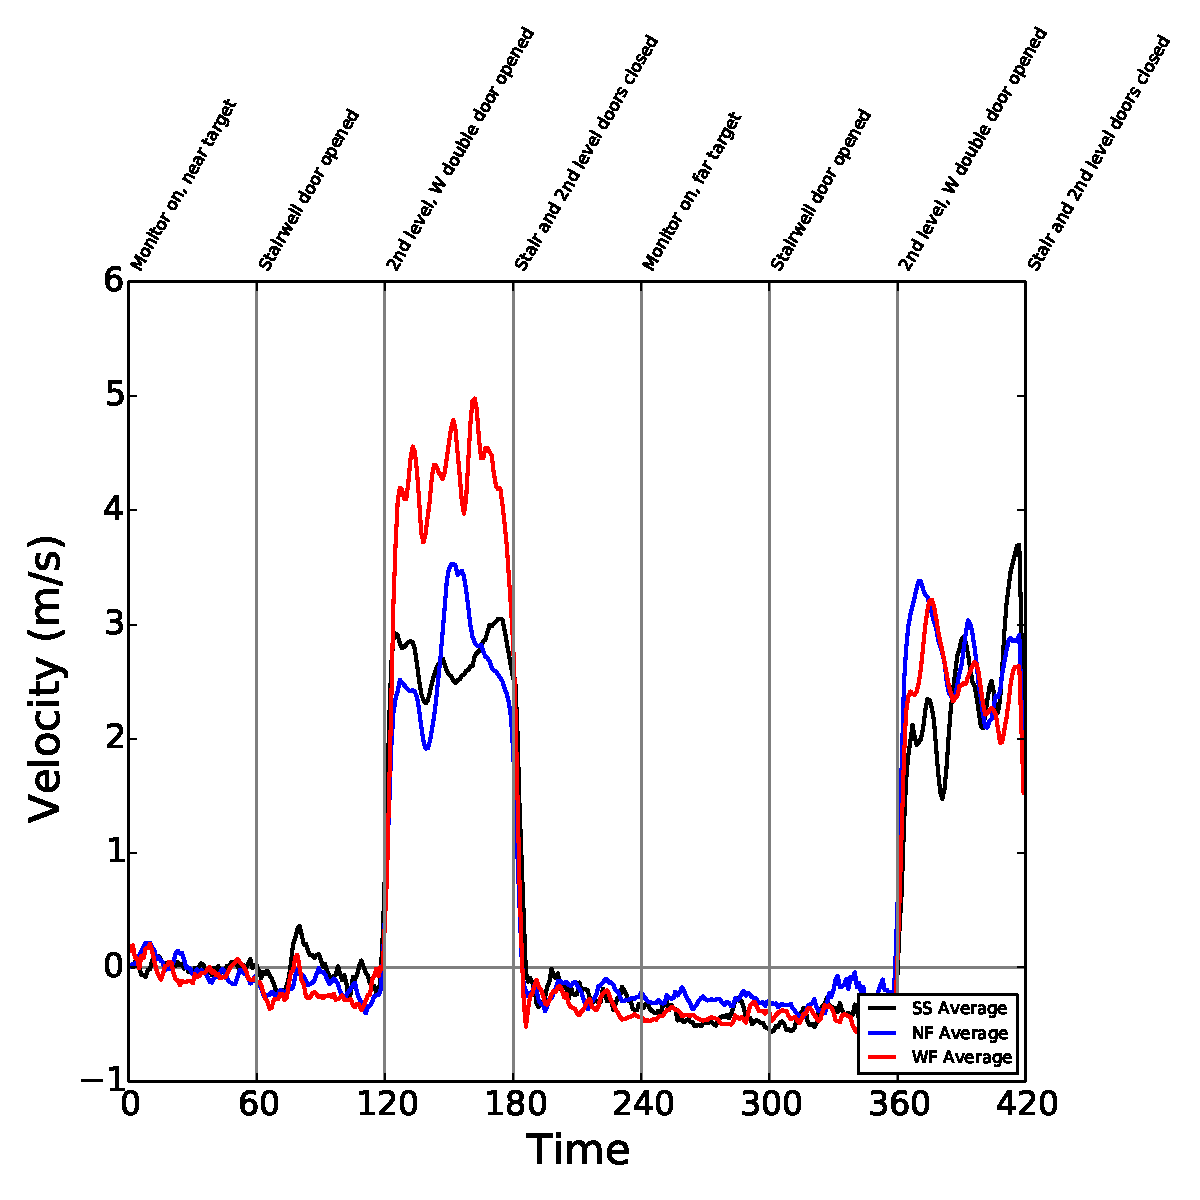
\includegraphics[width=6in]{../../../Figures/Hose_Test_Figures/Test_17_West_063014_BDP_A13_Avg}
\caption{Average Velocity through \nth{2} Level, North Side, West Double Door, Test 17, All Streams}
\label{fig:Test_17_BDP_A13_Avg_All}
\end{figure}

\clearpage


\end{document}

